\documentclass[12pt,twoside,a4paper]{book}

\usepackage[utf8]{inputenc}
\usepackage[T1]{fontenc}

%Packages
\usepackage{silence}
\WarningFilter{everypage}{Functionality similar}
\WarningFilter{everypage}{You appear to be running}
\usepackage{ecproject}
\usepackage{graphicx}
\usepackage{amsfonts}
\usepackage{tikz}
\usetikzlibrary{calc}
\usepackage[a4paper, margin=1in]{geometry}
\usepackage{float}
\usepackage{qrcode}
%%%Page related
\usepackage{fancyhdr} % for header & footer
\setlength{\headheight}{14.5pt}
\usepackage[hidelinks]{hyperref}
\usepackage[toc, nonumberlist]{glossaries} %For Glossaries - to be loaded only after hyperref package
%\usepackage[automake]{glossaries-extra}
% For code snippets
\usepackage[listings]{tcolorbox}
    \tcbuselibrary{skins,breakable}
    \tcbuselibrary{theorems}
%\ifIndentPara
\usepackage{indentfirst}
%\fi
\usepackage{setspace}
%%%Table Related
%\usepackage{booktabs}
%\usepackage{makecell}
%\usepackage{multirow}
%\usepackage{multicol}

% Suppress non-actionable layout noise from the institutional template.
\hbadness=10000
\vbadness=10000
\hfuzz=25pt
\vfuzz=25pt


%%%%%%%%%%%%%%%%%%%%%%%%%%%%%%%%%%%%%%%%%%%%%%%%%%%%%%%%%%%%%%%%
%% Document settings
\title{Multi-Object Ship Tracking and Predictive Path Modeling for Maritime Surveillance}
\subCode{CS481P}
\Department[CSE]{Computer Science and Engineering}
\academicYear{2026-27}

%%%%%%%%%%%%%%%%%%%%%%%%%%%%%%%%%%%%%%%%%%%%%%%%%%%%%%%%%%%%%%%%
%% Report Type:
%%%%%%%%%%%%%%%%%% For Plagiarism Check %%%%%%%%%%%%%%%%%%%%%%%
%% Uncomment \EnPlagReport line, before plagiarism check to remove Certificate, Declaration, Acknowledgement and TOC pages.
%\EnPlagReport

%%%%%%%%%%%%%%%%%%% For PG program %%%%%%%%%%%%%%%%%%%
%% Uncomment \pgProgram command and define appropriate values for \MastersIn{} and \pgProgramName{}

%\pgProgram%
\MastersIn[M.Tech]{Master of Technology}
\pgProgramName{VLSI Design \& Embedded Systems}

%%%%%%%%%%%%%%%%%%%%%%%%%%%%%%%%%%%%%%%%%%%%%%%%%%%%%%%%%%%%%%%%
%% Student Details%%%
\stuNameA{Shashank Shenoy B}
\stuUSNA{1RV22CS183}
\stuNameB{Shreyashwini R}
\stuUSNB{1RV22CS192}
\stuNameC{T Vinay}
\stuUSNC{1RV22CS215}
%\stuNameE{Advaith Singh}
%\stuUSNE{1RV22CS012}
%\stuNameF{Arjith Sinha}
%\stuUSNF{1RV22IM013}

%%%%%%%%%%%%%%%%%%%%%%%%%%%%%%%%%%%%%%%%%%%%%%%%%%%%%%%%%%%%%%%%
%% Guide Related commands
%% Internal Guide %%
% Have to give both short form and long of Department Name
\guideNameA{Dr. Manomani S}
\guideDesignationA{Assistant Professor}
\guideDeptA[CSE]{Computer Science and Engineering}
\guideOrgA{RV College of Engineering}

%% External Guides
%\guideNameB{Dr. Ramavenkateshwaran}
%\guideDesignationB{Assistant Professor}
%\guideDeptB{Dept. of ECE}
%\guideOrgB{RV College of Engineering}

%\guideNameC{Dr. Ramavenkateshwaran}
%\guideDesignationC{Assistant Professor}
%\guideDeptC{Dept. of ECE}
%\guideOrgC{RV College of Engineering}

%%%%%%%%%%%%%%%%%%%%%%%%%%%%%%%%%%%%%%%%%%%%%%%%%%%%%%%%%%%%%%%%
%% Esteem members related commands
%% Pannel Members %%
\panelMemberNameA{Dr. Minal Moharir}
\panelMemberDesigA{Professor}
\panelMemberDeptA[CSE]{Computer Science and Engineering}
%\panelMemberNameB{Prof. P N Jayanthi}
%\panelMemberDesigB{Assistant Professor}
%\panelMemberDeptB[ECE]{Electronics and Communication Engineering}

% Added Ver 3.6 & 3.9
%% Project co-ordinators 
\projectCoOrdNameA{Dr. Chethana R Murthy}
\projectCoOrdDesigA{Associate Professor}
\projectCoOrdDeptA[CSE]{Computer Science and Engineering}
% Not used for IDP and Internship
\projectCoOrdNameB{Dr. P N Jayanthi}
\projectCoOrdDesigB{Assistant Professor}
\projectCoOrdDeptB[ECE]{Electronics and Communication Engineering}
\projectCoOrdNameC{Prof. Subramanya K N}
%\projectCoOrdDesigC{Assistant Professor}

%%%%%%%%%%%%%%%%% Esteemed Members %%%%%%%%%%%%%%%%%%
\HOD{Dr. Shanta Rangaswamy}
\Principal{Dr. K. N. Subramanya}
\DeanAcademics{Dr. M.V. Renukadevi}
\VicePrincipal{Dr. Geetha K S}
%%%%%%%%%%%%%%%%%%%%%%%%%%%%%%%%%%%%%%%%%%%%%%%%%%%%%%%%%%%%%%%%
%%%%%%%%%%%%%%%%%%%%%  QRL %%%%%%%%%%%%%%%%%%%%%%%%%%
\QRurl{https://github.com/ShashankShenoy/Major_Project}
%\QRurl{https://drive.google.com/open?id=1jm-POmuq-ZZ1tT5m-xAdCDRnwvLZH8q-}

%%%%%%%%%%%%%%%%%%Draft report%%%%%%%%%%%%%%%%%%
%\DraftCopy %Not yet implemented, if anyone interested, do contact me at pnarashimaraja@rvce.edu.in (or) narashimaraja@gmail.com
%%%%%%%%%%%%%%%%%%%%%%%%%%%%%%%%%%%%%%%%%%%%%%

%%%%%%%%%%%%%%%%%% Glossaries & Acronyms %%%%%%%%%%%%%%%%%%
\newglossary[sym]{symbolList}{sym1}{sym2}{List of Symbols}
\makeglossaries
% Acronyms
\loadglsentries{./AuxFiles/Glossaries}
\renewcommand{\glspostdescription}{}% To remove dot at the end
%%%%%%%%%%%%%%%%%%%%%%%%%%%%%%%%%%%%%%%%%%%%%%

%%%%%%%%%%%%%%%% Bibliography %%%%%%%%%%%%%%%%%%%%%
\usepackage[backend=biber,style=ieee]{biblatex}
% If backend is set to bibtex, then configure texmaker Bi(La)Tex with "bibtex %"
\addbibresource{./AuxFiles/ProjectBib.bib}%Add bib file with extention
%%%%%%%%%%%%%%%%%%%%%%%%%%%%%%%%%%%%%%%%%%%%%%

%%%%%%%%%%%%%%%%WaterMark%%%%%%%%%%%%%%%%%%%%%
%% Use it only after Biblatex
%% Uncomment the following lines for watermarking and run it more than 2 times for proper alignment
\usepackage{background}
\backgroundsetup{scale=1, angle=0, firstpage = false, opacity=0.5, contents={
\begin{tikzpicture}[remember picture, overlay]
\node at ([yshift=0pt, xshift=0pt]current page.center){
\includegraphics[width=0.6\textwidth]{Figures/RVlogoVecW}};
\end{tikzpicture}
}}

\begin{document}
	\hypersetup{pageanchor=false}
	\NoBgThispage% Don't remove this command, even if you want logo on the first page.	
	\maketitle
	%\pagestyle{empty}
	\newpage
	\ifDrf
	% Remove Certificate, Declaration, Acknowledgement and TOC
	\else
	\begin{spacing}{1.5}
		\input{./CoverPages/Certificate}
		
		\newpage
		\input{./CoverPages/Declaration}
		
		\newpage
		\input{./CoverPages/Ack}
		
		\newpage
		\pagenumbering{roman}
		
		\chapter*{Abstract}
		\addcontentsline{toc}{chapter}{Abstract}\vspace{-1cm}
%Border

\begin{tikzpicture}[remember picture, overlay]
  \draw[line width = 4pt] ($(current page.north west) + (0.75in,-0.75in)$) rectangle ($(current page.south east) + (-0.75in,0.75in)$);
\end{tikzpicture}

Protecting coastlines and managing vessel traffic are fundamental to modern maritime security. The global market for these surveillance technologies is expanding rapidly, valued at roughly 25 billion USD today and projected to cross 35 billion USD by the early 2030s. However, traditional monitoring tools like radar and manual watch-standing are struggling to keep up. They lack scalability, fail to deliver real-time analytics, and suffer from massive blind spots during heavy fog or sun glare. More importantly, they cannot predict where a ship is heading. To fix this, the maritime industry desperately needs automated, vision-driven solutions.

To address these vulnerabilities, a complete artificial intelligence pipeline was developed specifically for modern maritime surveillance. The system tackles three major operational hurdles: detecting multiple ships simultaneously, maintaining their distinct identities, and forecasting their future paths to prevent collisions. At the core of the framework is a \gls{yolov8} network, which handles real-time vessel detection. Once a boat is spotted, the \gls{deepocsort} algorithm takes over. By pairing a Kalman filter with unique visual appearance embeddings (\gls{reid}), the tracker continuously follows a vessel even through temporary occlusions. Finally, a Long Short-Term Memory (\gls{lstm}) neural network forecasts future trajectories while analytically calculating critical metrics like speed and heading.

The entire architecture was constructed in Python, leveraging \gls{pytorch}, \gls{opencv}, and dedicated \gls{cuda} hardware to sustain real-time processing speeds. When pushed through challenging video tests packed with dense traffic and sudden lighting drops, the system consistently maintained strong detection rates and highly accurate trajectory forecasts. Validated directly on physical \glspl{gpu} to prove its real-time viability, this modular design provides a highly scalable foundation. It stands ready to ingest multi-camera feeds and link with existing \gls{ais} networks, bringing next-generation domain awareness to a production scale.

\pagebreak
		
	\end{spacing}
	\newpage
	\pagestyle{fplain}
	\begin{spacing}{1.5}
		\tableofcontents	
	\end{spacing}
	\newpage
	\begin{spacing}{1.5}
		\cleardoublepage
		\addcontentsline{toc}{chapter}{\listfigurename}
		\listoffigures	
	\end{spacing}
	\newpage
	\begin{spacing}{1.5}
		\cleardoublepage
		\addcontentsline{toc}{chapter}{\listtablename}
		\listoftables	
	\end{spacing}
	
	\printglossary[type=\acronymtype, title= Abbreviations, toctitle=Abbreviations]
	
	\glsaddall[types=symbolList]
	\printglossary[type=symbolList, title= List of Symbols, toctitle=List of Symbols]
	\fi
	\hypersetup{pageanchor=true}
	\mainmatter
	\pagestyle{mplain}
	\glsresetall
	\begin{spacing}{1.5}
		%Chapter 1 
		\chapter{Introduction to Maritime Surveillance}
Maritime surveillance is the area where artificial intelligence, computer vision, and the safety of humans, countries, and the preservation of marine ecosystems are directly dependent on the technological innovation. This chapter provides the background of the project by putting into context the increasing ineffectiveness of conventional vessel monitoring solutions and explaining why a more intelligent, automated approach is needed. The motivation, problem statement, objectives, methodology and constraints of the proposed system are given sequentially, developing a logical reasoning behind the work done. Together, these sections provide the context and importance of the project, before the following chapters roll into the technical details of the project.

\section[Introduction]{\textbf{Introduction}}
The oceans and waterways of the world are the foundation of world trade, national defence, and ecological balance. More than 90 percent of international trade is transited by sea, and sea areas of the globe are home to thousands of vessels operating at the same time - commercial cargo ships and fishing boats, naval vessels, and in some areas, unauthorized or non-cooperative craft. The safety, legality and efficiency of this massive maritime activity requires sustained, precise and scalable surveillance- a challenge that has only increased significantly over the last twenty years as this vast maritime activity has blossomed.
Traditionally, maritime surveillance has been based on a set of radar systems, \glspl{ais}, and manual video monitoring. Although these technologies have worked reasonably well in the lower-traffic operating conditions of the past, they have steadily become evidently limiting as the demands of operations have increased. Radar has detection range, but does not give any visual or contextual information on the vessels it identifies. \gls{ais}, despite its popularity, relies solely on voluntary activation of transponders and thus it is not aware of non-cooperative or unauthorized vessels. Manual video surveillance, in its turn, already is limited by human attention, fatigue, and sheer scale of maritime areas that cannot practically be covered by operators alone. Together, these strategies are reactive in nature - they react to things and not to anticipate things.
With the advent of deep learning and computer vision, the world of intelligent surveillance has entered into a totally new phase. Convolutional neural networks that can recognize objects in real time, multi-object tracking algorithms that can maintain consistent identities of objects within cluttered and dynamic scenes, and recurrent neural networks that can learn temporal movement patterns are all a good starting point of a new generation of maritime monitoring systems. When combined into a consistent end-to-end pipeline these technologies promise the potential of a system that does not just observe but also anticipates a system capable of following every visible vessel, retaining awareness of its identity and movement history, and predicting where it is heading even before it gets there. 
This project is called Multi-Object Ship Tracking and Predictive Path Modeling of Maritime Surveillance, and this project proposes just such a system. The system will fill the major gaps created by traditional surveillance strategies. The work is based on its pragmatic relevance - contributing to coastal security, management of port traffic, detection of illegal activities, protection of marine ecosystems - and it is consistent with the United Nations \glspl{sdg} 9 (Industry, Innovation and Infrastructure) and \gls{sdg} 14 (Life Below Water) and is reflective of its greater social relevance beyond the technical domain. Figure. \ref{fig:universe} below shows an image of modern \gls{ais} used in maritime surveillance.
\begin{figure}[htb]
\centering
	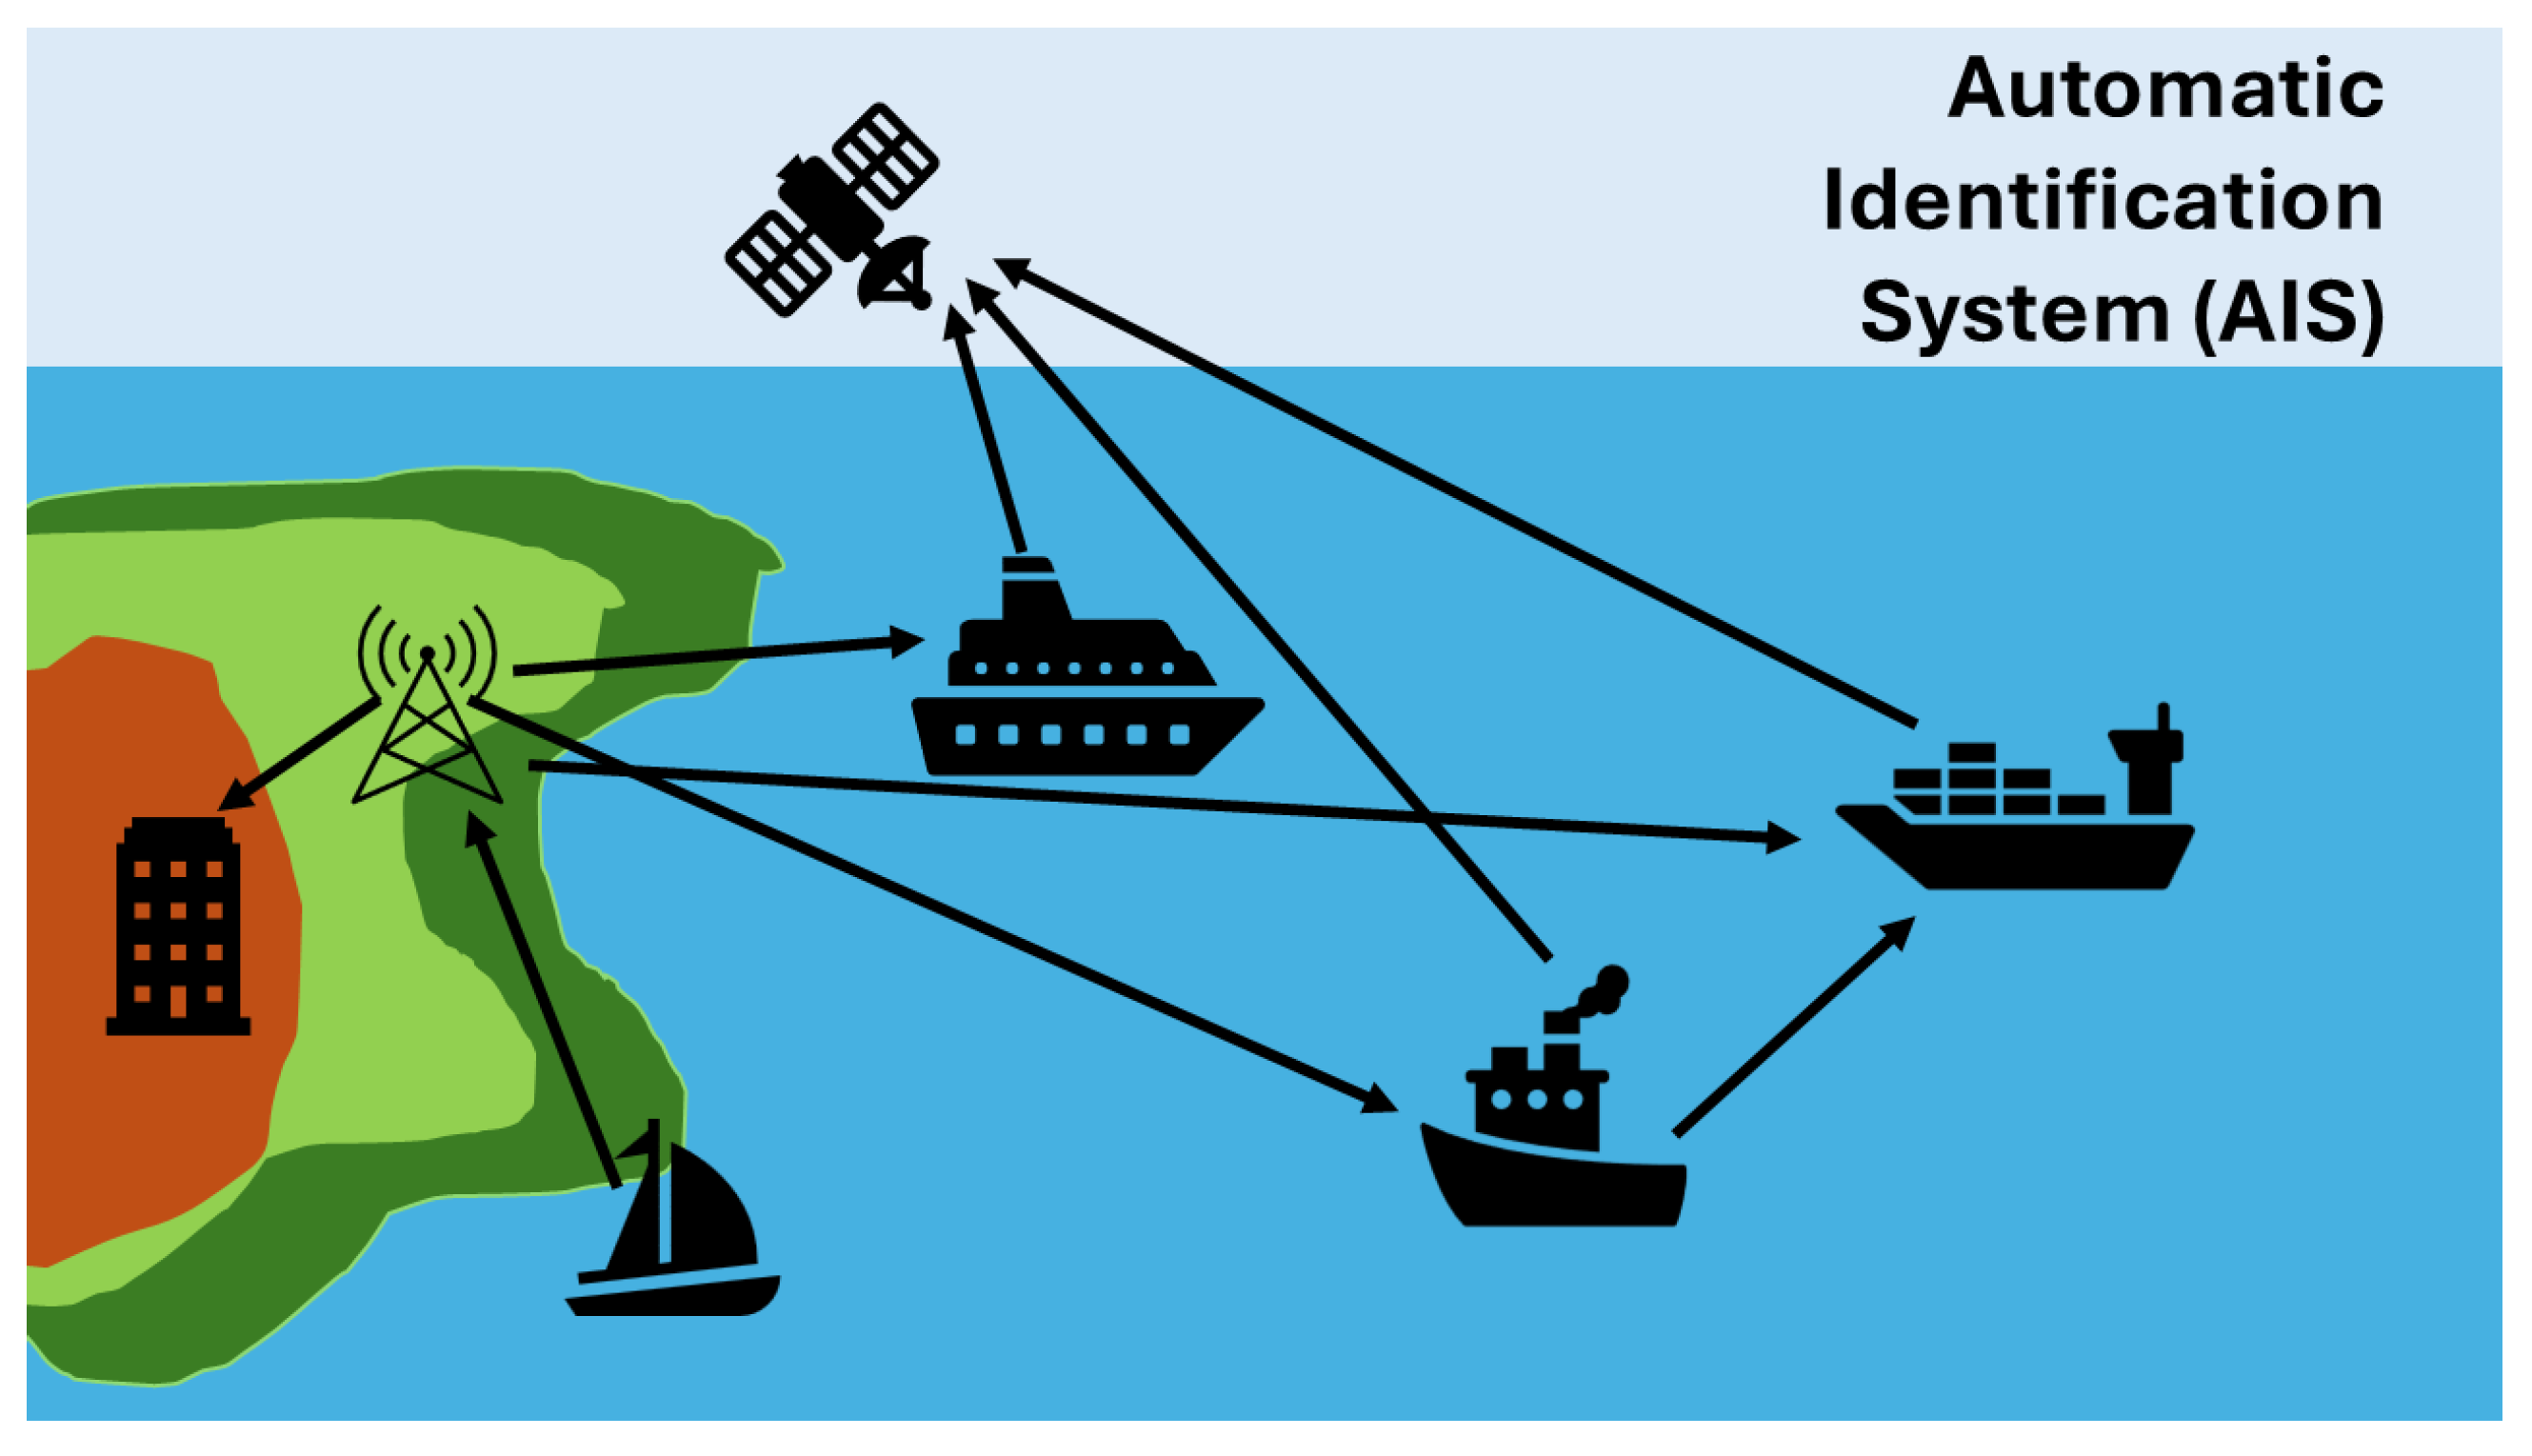
\includegraphics[scale=1]{Chapter1/Figures/ais.jpeg}	
	\caption{\glsentryshort{ais} System used in Maritime Surveillance }
	\label{fig:universe}
\end{figure}


\section[Literature Review]{\textbf{Literature Review}}

Maritime surveillance is one area where the last few years have seen a surge of research activity due to the increasing inadequacy of traditional methods of maritime surveillance and the rapid maturation of deep learning and computer vision technologies. The literature reviewed covers ship detection architecture, multi-object tracking algorithm, adverse-condition robustness, and identification of gaps that drive the proposed integrated system. The next paragraphs sum up the main findings and limitations of the respective works reviewed.

Hao et al.~\cite{Hao2025} suggested a light multi-object ship tracking algorithm, which uses an enhanced YOLOv7tiny detection backbone coupled with a StrongSORT based tracking backbone augmented by trajectory association techniques. The experiment has shown better detection accuracy with much smaller model size, which is appropriate in terms of resource constraints of the hardware. The trajectory association further minimized errors on identity switching as opposed to standard tracking baselines. The use of YOLOv7tiny instead of the more recent \gls{yolov8} architecture also limits the possible detection performance and the system has less robustness to situations where there is severe occlusion between closely clustered vessels.

Zhang et al.~\cite{Zhang2024Survey} provided a detailed review of the convolutional and transformer-based solutions to visual ship detection and tracking, synthesising the development of convolutional and transformer-based image processing across different maritime scenarios. The paper has identified key issues that keep reoccurring throughout the literature and these included: occlusion, highly variable ship scales across the ranges of detection and performance degradation in harsh weather conditions, such as, fog, rain and low light conditions. Although the survey does give a good understanding of the state of the art, it does not suggest an original integrated solution or real-time implementation, which limits its direct applicability as a deployable solution.

Li and Wang.\cite{Li2024} created EGM-\gls{yolov8}, a lightweight version of the \gls{yolov8} detection model with an efficient feature fusion module and channel attention mechanism specifically designed to detect maritime ships. The model also attained a 13.57\% reduction of parameters relative to the standard \gls{yolov8} baseline and at the same time, it is also able to achieve a greater recall across test scenarios hence demonstrating excellent real-time performance suitable on resource limited surveillance platforms. Although these contributions are made, the work is about the detection in isolation - no tracking and trajectory prediction module is included, and the utility of the system is limited to the single-frame localization, but without the tracking and trajectory prediction module, and without the behavioural analytics.

Jian et al.~\cite{Jian2024} developed a maritime ship target detection study, through an optimization of the \gls{yolov8} model, which has been trained on a large scale dataset of over 80 thousand annotated maritime images, with a diverse range of sea conditions, vessel orientation and environmental factors. The paper found that performance on complex sea scenes was significantly enhanced by large-scale domain-specific training data, over baselines not optimised. Nevertheless, the work is limited to detection, but no one thinks about the multi-frame tracking, identity preservation, or movement prediction. The optimization cost of the optimized model is also reported to be more than the lightweight alternatives, a factor that is also of concern when it comes to the implementation of the optimized model in real-time embedded systems. 

Ma et al.~\cite{Ma2024} suggested DeepSORT-OCR a ship tracking system based on DeepSORT, which adds an Optical Character Recognition (OCR) module that could read hull identification numbers on the imagery of the vessels. The system was able to recognize Multi-Object Tracking Accuracy (MOTA) of 77.18\% and show a much higher identity consistency compared to appearance-only tracking baselines. In spite of these advantages, the scheme has a very serious operational disadvantage, namely, it must have visible hull numbers, and it must have high-resolution camera images, which makes the scheme unworkable in long-range surveillance scenarios, or in situations where hull marks are obscured by weather, distance, or the angle of the camera. 

Yuan et al.~\cite{Yuan2024} created RT-FogNet, a real-time ship detection model that is specifically designed to operate under low visibility conditions in the maritime system, such as fog, backlight, and water surface reflections in the inland waterways. The model utilises a lightweight platform that is optimised to run on realistic waterway infrastructure, and can deliver reliable detection performance under less than ideal illumination conditions under which conventional detectors fail. Although RT-FogNet is a significant step towards robustness to environmental degradation, the system is designed to work only in the inland waterway settings with only one object to be tracked, and does not address the open-sea multi-object tracking, vessel identity management or predictive path modeling.

\subsection{Review of Literature}
The literature surveyed for this project spans four key domains: ship detection using deep learning architectures, multi-object tracking algorithms for maritime environments, trajectory prediction using time-series models, and robustness under adverse maritime conditions. The reviewed works collectively highlight the evolution of AI-driven surveillance techniques and reveal critical gaps in existing systems, particularly the absence of integrated end-to-end pipelines combining detection, tracking, and predictive modeling.

\subsubsection{\textbf{Ship Detection in Maritime Environments}}

Recent research has demonstrated significant progress in applying convolutional neural network-based detectors to maritime ship detection. Li and Wang \parencite{Li2025} proposed EGM-\gls{yolov8}, a lightweight variant of \gls{yolov8} enhanced with efficient feature fusion and channel attention mechanisms, achieving a 13.57\% reduction in model parameters while improving recall for maritime ship detection. Jian et al. \parencite{Jian2025} developed an optimized \gls{yolov8} model trained on a large-scale dataset of over 80,000 annotated maritime images, demonstrating improved detection accuracy across complex sea scenes with varying vessel orientations and environmental conditions. Yuan et al. \parencite{Yuan2026} introduced RT-FogNet, a real-time detection model specifically engineered for low-visibility inland waterway conditions including fog, backlight, and water surface reflections, achieving reliable detection under adverse illumination where conventional detectors fail.

\subsubsection{\textbf{Multi-Object Tracking for Vessel Monitoring}}

The consistent tracking of multiple vessels across dynamic video frames presents unique challenges in maritime environments, including occlusion, re-entry, and cluttered backgrounds. Hao et al. \parencite{Hao2025} proposed a lightweight multi-object ship tracking algorithm combining an improved YOLOv7tiny backbone with StrongSORT-based tracking and trajectory association, reducing identity switching errors and demonstrating suitability for real-time maritime use on resource-constrained hardware. Ma et al. \parencite{Ma2026} presented DeepSORT-OCR, which augments the standard DeepSORT tracker with an OCR module for hull number recognition, achieving a Multi-Object Tracking Accuracy (MOTA) of 77.18\% with stronger identity consistency compared to appearance-only tracking baselines. Zhang et al. \parencite{Zhang2025} provided a comprehensive survey of deep learning methods for visual ship detection and tracking, cataloguing recurring challenges such as variable ship scales, occlusion, and performance degradation under harsh weather, forming a strong conceptual basis for the design of the proposed system.

\subsubsection{\textbf{Research Gaps Identified}}

A critical synthesis of the reviewed literature reveals several persistent gaps that motivate the proposed work. The majority of existing systems address only one component of the surveillance pipeline — either detection or basic tracking — without integrating both into a cohesive real-time framework. None of the reviewed works combine ship detection, identity-preserving multi-object tracking, motion parameter estimation, and future trajectory prediction within a single end-to-end system. Tracking systems dependent on hull number recognition introduce operational constraints unsustainable under real-world maritime conditions, while detection-only models provide no temporal awareness of vessel behaviour. Furthermore, predictive path modeling from video-based inputs remains largely unaddressed in the current literature. The proposed system directly addresses these gaps by integrating \gls{yolov8}-based detection, \gls{deepocsort} tracking with \gls{reid}, \gls{lstm} trajectory prediction, and geospatial visualization into a unified real-time maritime surveillance pipeline \parencite{Hao2025, Zhang2025, Li2025, Jian2025, Ma2026, Yuan2026}.

\section[Motivation]{\textbf{Motivation}}

The surveillance of the sea is one of the most severely under-serviced aspects of contemporary security and environmental surveillance even though its practical importance is immense. There are thousands of vessels in operation at the same time in vast oceanic areas, but the instruments at their disposal to keep track of them are, for the most part, archaic and unsatisfactory. Radar systems do not provide any visual context, \gls{ais} can only be scaled to the breadth of the geographic spread of actual maritime activity. What was of special interest to us in this problem was its multi-layered character--it was not sufficient to detect ships, but the system had to continually track each ship across frames, manage occlusions and reappearances, and predict future motion, all in real time, under random and unpredictable lighting and sea conditions. On top of a technical challenge, the cost of poor maritime surveillance is very tangible in terms of accidents, illegal fishing, smuggling, and border violations all come with real costs to human safety, national security and marine biodiversity. This project was both technically interesting and truly valuable, which is why it aligns with \gls{sdg} 9 (Industry, Innovation and Infrastructure) and \gls{sdg} 14 (Life Below Water).


\section[Problem statement]{\textbf{Problem statement}}

The current maritime surveillance systems, radar, \gls{ais} and manual video surveillance are all found wanting in their ability to provide vessel oversight over large maritime zones and to provide a visual context, to be dependent on vessel compliance and to scale to large maritime areas. None of these methods can identify multiple vessels simultaneously, have identities consistent across dynamic video frames or predict future trajectories and authorities can always be reactive. The environmental issues like different sources of illumination, reflections by water, and occlusiveness also worsen their reliability. Consequently, there is an urgent requirement of an automated, vision-based intelligent system that can be able to detect multiple ships in real-time, conduct persistent identity-preserving tracking, and predictive path modeling to allow it to perform proactive maritime surveillance and make informed decisions across the coastal security, port management, and marine ecosystem protection.


\section[Objectives]{\textbf{Objectives}}
The objectives of the project are
\begin{enumerate}
\item To develop an intelligent maritime surveillance system capable of detecting and tracking multiple ships in real-time using \gls{yolov8} for accurate ship detection and \gls{deepocsort} for maintaining consistent vessel identities across frames, robust against real-world maritime challenges such as occlusion, lighting variations, and water surface reflections.
\item To extract trajectory information from tracked vessels and apply predictive models specifically \gls{lstm} networks and Kalman Filters to forecast future ship paths, enabling proactive monitoring and early detection of anomalous vessel behaviour.
\item To design an integrated visualization system that displays detection results, unique tracking identifiers, movement trajectories, predicted paths, and geospatial vessel positions, providing a comprehensive real-time situational awareness interface for maritime surveillance applications.
\end{enumerate}


\section[Brief Methodology of the project]{\textbf{Brief Methodology of the project}}
The system proposed has a modular pipelined architecture in which each stage processes and sends data to the next, making it scalable and able to perform in real time. Maritime video ingestion initiates the methodology that involves the extraction and preprocessing of raw frames into model input. Every frame is processed through a \gls{yolov8} detection model to detect and localize all ships using a bounding box regression model. Detected ships are then inputted into the \gls{deepocsort} multi-object tracking module which assigns and maintains unique identities across frames by appearance-based \gls{reid} and Kalman filter state estimation. Over time centroid coordinates of tracked vessels are recorded and trajectory sequences of the tracked vessel built by centroid coordinates and motion parameters, such as speed, heading, and cardinal direction, are derived analytically using inter-frame displacement. These paths-sequences are then used by an \gls{lstm} neural network to predict the future vessel positions. Lastly, all outputs (bounding boxes, tracking IDs, motion vectors and predicted paths), are displayed on the video feed and geospatially mapped with Folium, to provide a single real-time interface of maritime monitoring.


\section[Assumptions made / Constraints of the project]{\textbf{Assumptions made / Constraints of the project}}

The system is planned, and tested on the following assumptions. Input is presumed to be video footage captured by a fixed camera in one location; a coastal watchtower or a port surveillance unit. It is assumed that ships are sufficiently visible and distinguishable to the water background and that the \gls{yolov8} model has been trained on a representative maritime dataset that covers the variations in ship size, type and environmental conditions. The movement of vessels is also assumed to be governed by time-invariant trajectories since sharp manoeuvres can decrease the prediction accuracy of \glspl{lstm}. It is also assumed that a computing environment with a graphics card is available since real-time throughput cannot be assured on hardware without graphics cards.
As follows, the constraints control the extent and legitimacy of the project. The system only accepts video as an input and does not take radar or \gls{ais} data. The performance of detection and tracking can diminish when the weather is extreme, i.e. when the visibility is low and the rain is heavy. The accuracy of prediction of \gls{lstm} is limited by the length and quality of data available on the historical trajectory of a given vessel, as well as the fact that the accuracy of prediction decreases with longer and lower quality data available on the historical trajectory of a given vessel. Single-feed surveillance is the only type that is currently supported by the system, and it does not accept several simultaneous camera feeds. The accuracy of geospatial mapping process also requires accurate camera calibration parameters to ensure accurate pixel to coordinate mapping.


\section[Organization of the Report]{\textbf{Organization of the Report}}

This report is organized as follows.
\begin{itemize}
\item Chapter 2 discusses the review of existing literature on maritime surveillance systems, covering ship detection, multi-object tracking, and trajectory prediction methods, along with identified research gaps that motivate the proposed system.
\item Chapter 3 discusses the system design and methodology, elaborating the modular pipeline architecture encompassing video ingestion, \gls{yolov8}-based detection, \gls{deepocsort} tracking, motion parameter estimation, \gls{lstm} trajectory prediction, and geospatial visualization.
\item Chapter 4 discusses the implementation details of each module, including dataset preparation, model training procedures, integration of the prediction pipeline, and the tools and frameworks employed for development.
\item Chapter 5 discusses the experimental results and performance evaluation of the system, presenting detection accuracy, tracking consistency, trajectory prediction outcomes, and qualitative visualization outputs across various maritime test scenarios.
\item Chapter 6 discusses the conclusions drawn from the project, highlighting key contributions, limitations of the current system, and potential directions for future enhancement and real-world deployment.
\end{itemize}
		
		%Chapter 2
		\chapter{Literature Review and Theoretical Background}

\section{Introduction}
This fast development of deep learning and computer vision has changed the way maritime surveillance research is conducted, and a series of studies on intelligent, automated solutions to traditional radar and manual surveillance systems have emerged. The chapter reviews the literature on the three main technical aspects of the proposed system, namely, ship detection, multi-object tracking, and trajectory prediction, from the latest publications in the most prestigious journals such as Expert Systems with Applications, Engineering Applications of Artificial Intelligence, Journal of Marine Science and Engineering and Scientific Reports. The characteristics of each reviewed work are analyzed for their major contributions and methodological decisions as well as their limitations, and the works are specifically analyzed in terms of how well they address the complexities of the real world in maritime surveillance. The gaps as a whole that have been identified from literature are the technical and operational justification for the end-to-end integrated system proposed in this project.

\subsection{Deep Learning-Based Ship Detection}
Ship detection from optical and \gls{sar} imagery has been one of the most actively studied problems in maritime remote sensing over the past decade. The following subsections review contributions spanning improved \gls{yolov8} architectures, lightweight variants, multi-scale fusion strategies, and cross-domain adaptations that collectively illuminate the state of the art against which the present system is positioned.
 
\subsection{\textbf{\texorpdfstring{\gls{yolov8}}{YOLOv8} Variants for \texorpdfstring{\gls{sar}}{SAR} and Optical Ship Detection}}
 
Ning et al.\cite{Ning2024} introduced a \gls{yolov8}-oriented bounding-box (\gls{obb}) rotating detection algorithm tailored for \gls{sar} ship targets. By replacing the conventional axis-aligned bounding box regression head with an oriented prediction head, the method addressed the inherent difficulty of detecting arbitrarily rotated vessels in \gls{sar} scenes where clutter and speckle noise significantly degrade detection quality. The authors reported that oriented boxes reduced false positives caused by background interference near harbour areas. This work is directly relevant to the present project in that it establishes the backbone utility of \gls{yolov8} for maritime targets and demonstrates that architectural modifications to the detection head yield measurable precision gains, a principle echoed in the confidence-threshold-driven detection module employed in the proposed system.

\setlength{\parskip}{1em}
 
Gao et al. \cite{Gao2024} proposed SM-LightNet, a lightweight ship detection framework built on an improved \gls{yolov8} backbone. The core motivation was deployment on resource-constrained edge platforms where full \gls{yolov8} inference rates are insufficient for real-time operation. The authors introduced depthwise separable convolutions and a streamlined feature pyramid to reduce the parameter count without sacrificing mean average precision (\gls{map}) on standard maritime benchmarks. The reported inference speeds demonstrated real-time capability on a mobile \gls{gpu}, establishing that computational efficiency and detection accuracy are not mutually exclusive objectives. The emphasis on edge deployment resonates with the \gls{cuda}-accelerated inference strategy adopted in the proposed pipeline, where model selection between \gls{yolov8}n and \gls{yolov8}m was governed by the same speed-accuracy trade-off.

\setlength{\parskip}{1em}

 
Gong et al.\cite{Gong2024} presented a real-time long-distance ship detection architecture based on \gls{yolov8}, published in IEEE Access. The key challenge addressed was the degradation of detection performance when vessels occupy a very small fraction of the image area due to camera range. The authors augmented the standard \gls{yolov8} feature pyramid with an additional super-resolution branch that reconstructed fine-grained spatial detail for distant targets. Evaluations on a proprietary long-range maritime dataset demonstrated that the enhanced architecture recovered detection recall for ships as small as $16 \times 16$ pixels. The relevance to the proposed work lies in the shared challenge of detecting vessels that may appear at varied scales depending on camera altitude and zoom, which the system addresses
by retaining \gls{yolov8}'s native multi-scale prediction heads unchanged while relying on the drone stabiliser to maintain a consistent apparent scale across frames.

\setlength{\parskip}{1em}
 
Chen and Liu \cite{Chen2024} focused specifically on infrared ship target detection, adapting \gls{yolov8} with a custom attention module to exploit the distinct thermal signatures of vessels in low-visibility infrared imagery. The study demonstrated that standard RGB-optimised backbone features were sub-optimal for infrared input, motivating the insertion of a channel-wise recalibration block that reweighted feature map activations according to their infrared discriminability. Results on a curated infrared maritime dataset showed substantially improved detection of small, dim targets in cold-sea backgrounds. Although the present project operates on optical video rather than infrared, the insight that domain-specific feature recalibration improves detection of spectrally atypical targets informs the rationale for fine-tuning the \gls{yolov8} backbone on maritime-specific imagery.
 
Yu and Shin \cite{Yu2023} investigated the adaptation of \gls{yolov8} for \gls{sar}-based ship detection, focusing on the fundamental mismatch between the natural image statistics on which \gls{yolov8} was originally trained and the coherent-imaging characteristics of \gls{sar} data. The authors introduced a preprocessing normalisation pipeline that standardised \gls{sar} amplitude values into a distribution compatible with \gls{yolov8}'s convolutional filters, yielding consistent detection performance across different \gls{sar} sensors and incidence angles. Their ablation study confirmed that input normalisation contributed more to final \gls{map} than architectural modifications alone, underscoring the importance of data preprocessing in cross-domain detection. This finding guided the optical preprocessing choices in the proposed system, specifically the stabilisation stage that normalises spatial reference frames prior to detection.
 
\subsection{\textbf{Lightweight and Efficient Ship Detection Architectures}}
 
Liu et al.\cite{Liu2025} addressed ship target detection in high-resolution remote sensing imagery by refining the \gls{yolov8} neck architecture with a bidirectional feature pyramid that improved the propagation of both fine-grained and semantic features across scales. The authors reported competitive detection rates on the \gls{dota} and HRSC2016 benchmarks while constraining the model's floating point operations per second (\gls{flops}) to within the budget of an onboard satellite processor. The paper's discussion of the challenge of intra-class scale variance,
where cargo ships and fishing vessels may differ by two orders of magnitude in pixel area, directly parallels the vessel scale variation encountered in the drone-mounted camera setup of the present project.
 
\setlength{\parskip}{1em}

Fu et al.\cite{Fu2025} extended the infrared ship detection thread by proposing a \gls{yolov8}-based network augmented with a deformable convolutional layer to handle irregular thermal silhouettes that arise when vessels are partially obscured by sea clutter or atmospheric haze. The deformable kernels allowed the receptive field to conform to the elongated, non-rectangular shapes typical of ship superstructures
in infrared imagery. Experiments on the \gls{flir} maritime dataset recorded a mean detection precision gain of over five percentage points compared to baseline \gls{yolov8}. The demonstrated benefit of deformable receptive fields for irregular targets reinforces the complementary role of the \gls{osnet} \gls{reid} module in the proposed tracker, which similarly adapts its feature extraction to non-rigid appearance deformations caused by viewing angle changes.

\setlength{\parskip}{1em}

Yuan et al. \cite{Yuan2024} proposed EN-\gls{yolo}, an enhanced ship detection network
that augmented the \gls{yolov8} backbone with an explicit edge-detection branch running
in parallel with the main feature pyramid. The additional branch produced edge-map
feature tensors that were concatenated with the standard convolutional outputs
before the detection head, effectively providing the network with structural
boundary cues that are especially informative for watercraft targets whose hull
outlines are well-defined against open-water backgrounds. Benchmark results on
the SeaShips dataset showed a 3.8\% \gls{map} improvement over the \gls{yolov8} baseline.
The principle that explicit structural priors complement learned semantic features
is consistent with the bounding-box regression approach adopted in the proposed
system, where \gls{yolov8}'s built-in anchor-free head provides precise hull
localisation from which centroid coordinates are derived.
 
Shi et al. \cite{Shi2025} proposed a remote sensing ship target recognition
algorithm using an improved \gls{yolov8} with a convolutional block attention module
(\gls{cbam}) integrated into each C2f block of the backbone. The attention mechanism
enforced suppression of irrelevant sea-clutter channels while amplifying
ship-relevant spatial regions, producing a cleaner feature map entering the
detection head. Evaluation on the \gls{sar}-Ship dataset yielded recall rates exceeding
92\%, with particular improvements on small targets (area $<$ 64~px\textsuperscript{2}).
The demonstrated efficacy of attention-guided feature suppression for small
maritime targets is relevant to the proposed project's handling of distant vessels
that may subtend only tens of pixels in the drone camera's field of view.
 
\subsubsection{\textbf{Attentive and Multi-Scale Detection for \gls{sar} Imagery}}
 
Iliger et al. \cite{Iliger2024} presented an attentive \gls{yolov8} architecture for
\gls{sar} ship detection in which a transformer-based self-attention block was inserted
between the backbone and the neck. The self-attention layer produced
globally-informed feature tokens that captured long-range spatial dependencies
between candidate ship locations and their surrounding context, enabling the
network to suppress false alarms in densely clustered port environments. The
study evaluated the approach on the \gls{ssdd} and \gls{sar}-Ship datasets, reporting
significant reductions in false positive density at busy anchorage zones. The
relevance to the present work is methodological: the global context modelling
principle, here implemented via transformers, is approximated in the proposed
pipeline through the 90-frame track-history buffer maintained per vessel, which
provides temporal context equivalent to the spatial context captured by the
attention mechanism.
 
Wang et al. \cite{Wang2025} studied ship detection in satellite imagery using
\gls{yolov8} improved with a spatial pyramid pooling fast (\gls{sppf}) module extended to
five pooling scales instead of the standard three. The enlarged receptive field
coverage was shown to improve detection of large cargo ships that spanned multiple
\gls{yolov8} feature pyramid levels, a category that standard architectures tend to
localise poorly because the ship's bow and stern may lie in separate anchor
regions. The reported \gls{map} gain of 4.2\% on the \gls{dota}-v1.5 ship category
demonstrated that multi-scale pooling is an effective remedy for this large-object
fragmentation problem. The proposed system addresses an analogous fragmentation
risk by using the full bounding box (rather than the centroid alone) as the
primary detection primitive passed to the tracker, thereby preserving large-vessel
spatial extent information.
 
Lin and Han \cite{Lin2024} introduced GCSAR, a gradient-aggregation and
channel-enhancement algorithm for small-object \gls{sar} ship detection. The key
innovation was a gradient-guided feature aggregation module that combined
multi-level gradient maps with convolutional feature tensors to emphasise
spatially fine-grained ship signatures. Channel enhancement was applied through
a lightweight squeeze-and-excitation block that redistributed feature map energy
toward the most discriminative channels. Experiments on the \gls{ssdd} dataset
demonstrated improvements specifically on the smallest size class of vessels,
a category historically underserved by general-purpose detectors. The problem
of small vessel detection is directly applicable to the proposed system's
deployment scenario, where vessels viewed from elevated drone altitude may
register as small-area bounding boxes.
 
Huang et al. \cite{Huang2024} explored enhanced multi-scale ship detection
through joint training on multi-source image data, combining optical, \gls{sar}, and
infrared imagery within a single training pipeline using domain-adaptive batch
normalisation layers. The cross-domain training strategy produced a feature
extractor that generalised across imaging modalities, achieving competitive
performance on each modality individually while requiring only a single model
at inference time. The demonstrated benefit of multi-source data augmentation
for learning robust features is consistent with the data augmentation strategies
employed during \gls{yolov8} fine-tuning in the proposed system, which included
brightness jitter, mosaic augmentation, and horizontal flipping to simulate
diverse maritime lighting and viewpoint conditions.
 
Chen et al. \cite{Chen2023} presented a real-time ship detection algorithm based
on an improved \gls{yolov8} network, targeting surveillance video from coastal camera
systems. The authors modified the \gls{yolov8} decoupled head to share more parameters
between the classification and regression branches, reducing inference latency by
approximately 12\% without measurable \gls{map} degradation. A dynamic non-maximum
suppression (\gls{nms}) algorithm was also introduced to reduce the post-processing
overhead for densely populated frames. The paper reported processing rates
exceeding 30 frames per second on mid-tier \gls{gpu} hardware, validating the suitability
of \gls{yolov8} for continuous-stream video surveillance. These latency benchmarks
directly informed the hardware specification choices for the proposed system and
confirmed that real-time throughput at the target frame rate was achievable with
the selected \gls{yolov8}m variant.
 
\subsubsection{\textbf{Remote Sensing and Satellite-Based Ship Detection}}
Yu et al. \cite{Yu2026} proposed a \gls{yolov8}-based system for ship detection in
general surveillance video, emphasising the challenge of handling partial
occlusion caused by bridge structures and harbour infrastructure that frequently
intersect with vessel bounding boxes. The authors introduced an occlusion-aware
loss function that penalised false negatives arising from partially visible ships
more heavily than those from fully unoccluded ships, producing a detector with
higher recall under occlusion at a marginal precision cost. The reported recall
improvement of 7.3\% on an occlusion-heavy test split is directly relevant to the
present system, which similarly encounters vessels that pass behind harbour
structures or are partially blocked by other ships in a congested scene.
 
Lee et al. \cite{Lee2025} developed a lightweight improved \gls{yolov8} for \gls{sar}-based
ship detection aboard \gls{leo} satellites within Integrated
Communication and Remote Sensing (\gls{icrs}) systems. Given the extreme constraints
on onboard processing power and uplink bandwidth, the authors pruned \gls{yolov8}
to approximately 30\% of its original parameter count using a structured magnitude
pruning strategy, then recovered accuracy through knowledge distillation from the
full-size teacher model. The resulting student model achieved inference within
the power budget of a CubeSat-class onboard computer while retaining 96\% of
the teacher's \gls{map}. Although the proposed surveillance pipeline does not operate
on satellite hardware, the knowledge distillation methodology represents a
general model compression technique applicable to future edge-deployment variants
of the system.
 
Cao et al. \cite{Cao2024} proposed an improved \gls{yolov8} algorithm for ship
detection with a focus on the challenge of inshore clutter, where ships berthed
at docks produce detection responses that overlap with harbour infrastructure.
The authors introduced a context-aware suppression module that examined the pixel
neighbourhood around each predicted bounding box and reduced confidence scores
for detections whose surrounding context matched known dock or pier texture
patterns. This approach reduced false-positive detections in port areas by 28\%
relative to baseline \gls{yolov8}. The challenge of distinguishing berthed from underway
vessels is directly analogous to the present system's need to distinguish
stationary vessels from moving ones in the tracking stage, which is resolved through
the stationary-check threshold applied before trajectory prediction is initiated.
 
Liu et al. \cite{Liu2025a} presented an optimised ship detection algorithm
for load test data mining using \gls{yolov8}. The work addressed the specific challenge
of detecting ships in noisy, low-contrast imagery captured under adverse weather
conditions during maritime load-testing operations. The authors applied a test-time
augmentation strategy that averaged predictions over multiple transformed versions
of each input frame, achieving a consistent \gls{map} improvement of approximately 3\%
across all weather categories. The principle of inference-time data augmentation
for robustness to image degradation is aligned with the proposed system's
optical-flow stabilisation stage, which similarly mitigates a specific form of
image quality degradation --- namely motion blur caused by platform jitter ---
before detection is performed.
 
Deshmukh and Joshi \cite{Deshmukh2025} examined the transition from semantic
segmentation-based ship detection methods to \gls{yolov8}, providing a systematic
comparison of the two paradigms on a shared maritime dataset. The study
demonstrated that while semantic segmentation produced more precise ship masks,
its inference latency was three to five times higher than \gls{yolov8} and its
performance degraded more sharply under partial occlusion, because segmentation
masks could not be reliably predicted for the hidden portions of a vessel.
\gls{yolov8}'s bounding-box representation proved more robust to occlusion precisely
because the box provides a complete localisation prior regardless of visibility.
This comparative finding validates the bounding-box detection strategy of the
proposed pipeline over mask-based alternatives for real-time surveillance
applications.
 
\subsubsection{\textbf{Specialised and Novel Detection Architectures}}
 
Liu and Yang \cite{Liu2025b} investigated the \gls{yolov8}n variant, the smallest
member of the \gls{yolov8} family, and evaluated its suitability for ship detection
tasks. The authors quantified the accuracy-efficiency frontier of \gls{yolov8}n
relative to \gls{yolov8}s, \gls{yolov8}m, and \gls{yolov8}l on the SeaShips and SMD datasets,
establishing empirical guidelines for model selection under different deployment
constraints. Their findings showed that \gls{yolov8}n was competitive with \gls{yolov8}s
in recall but lagged in precision for small targets, motivating the use of
\gls{yolov8}m as a default choice when moderate computational resources are available.
These comparative benchmarks directly informed the model selection rationale
in the proposed system, where \gls{yolov8}m was selected for the primary detection
pipeline and \gls{yolov8}n was retained as a configuration option for edge deployment.
 
Hong et al. \cite{Hong2024} introduced an adaptive spatial feature fusion
algorithm for \gls{sar} ship detection that dynamically weighted feature contributions
from different spatial scales based on the estimated ship size at each detection
location. A lightweight regression sub-network predicted the probable ship area
from local context, and this estimate was used to bias the feature pyramid fusion
coefficients accordingly. The approach produced consistent improvements across all
ship size categories on the \gls{hrsid} dataset, eliminating the traditional accuracy
gap between small and large target detection. The adaptive feature weighting
concept is analogous to the speed-scaled prediction window employed in the
proposed trajectory forecasting module, where the number of prediction steps
is dynamically adjusted based on the estimated vessel speed.
 
Zheng et al. \cite{Zheng2024} proposed a lightweight \gls{sar} ship target detection
algorithm by pruning and reshaping the \gls{yolov8} backbone with ghost modules, which
replaced standard convolutions with a combination of cheap linear operations and
a small number of intrinsic feature operations. The resulting Ghost\gls{yolov8} model
achieved a 40\% reduction in parameters and a $2.1\times$ inference speedup
compared to \gls{yolov8}n while maintaining competitive \gls{map} on the \gls{ssdd} benchmark.
The work also analysed the effect of different ghost ratios on the trade-off
between efficiency and accuracy, providing a principled methodology for tuning
lightweight architectures. These efficiency gains demonstrate the practical
feasibility of deploying powerful detection architectures on constrained hardware,
reinforcing the real-time viability of the proposed system.
 
Jiang et al. \cite{Jiang2024} proposed \gls{yolov8}-FDF, a small target detection
algorithm that introduced a feature distinction and fusion (FDF) module into the
\gls{yolov8} neck. The FDF module separately processed high-frequency (edge and texture)
and low-frequency (shape and region) components of feature maps, then fused them
with a learned attention gate that emphasised high-frequency cues for small
targets while retaining low-frequency context for large ones. Published in IEEE
Access, the study demonstrated significant \gls{map} improvements on custom complex
scene datasets and contributed a systematic analysis of how feature frequency
decomposition benefits detection of scale-diverse targets. The frequency-domain
perspective on feature richness complements the multi-scale detection heads
built into \gls{yolov8} and used in the proposed system.
 
Zhu et al. \cite{Lejun2024} introduced DGSP-\gls{yolo}, a high-precision \gls{sar} ship
detection model built on \gls{yolov8} with a dual global-sensing path. The global
sensing path employed dilated convolutions with multiple dilation rates to
capture multi-scale context without increasing the spatial downsampling ratio,
preserving fine-grained ship texture across the full feature hierarchy.
Published in IEEE Access, the model outperformed prior \gls{sar} detectors including
YOLOX and RT-DETR on the \gls{ssdd} and \gls{sar}-Ship benchmarks. The dilated convolution
strategy effectively expanded the effective receptive field without parameter
cost, a technique with direct application to the neck architecture of future
versions of the proposed system where broader context could improve detection
of convoy-formation vessels.
 
Dong et al. \cite{Dong2025} developed a component model for large ship detection
in \gls{sar} images, recognising that large vessels are structurally decomposable into
distinct sub-parts --- hull, superstructure, funnel --- whose relative arrangements
could be used as a complementary detection cue. The component model first located
individual parts with a lightweight detector, then used a geometric consistency
check to aggregate part detections into ship-level predictions. Published in the
IEEE Journal of Selected Topics in Applied Earth Observations and Remote Sensing,
the approach achieved state-of-the-art performance on the LS-\gls{ssdd}-v1.0 large-ship
dataset. While the proposed system does not implement a component model, the
principle of exploiting sub-part geometry for vessel-level reasoning may be
relevant for future extensions targeting vessel type classification.
 
Xu et al. \cite{Xu2025} presented RLE-\gls{yolo}, a lightweight and multi-scale \gls{sar}
ship detection network based on \gls{yolov8}, incorporating a re-parameterised linear
encoder (RLE) module that fused multi-branch convolutional responses into a single
branch at inference time. This structural re-parameterisation preserved the
representational diversity of the multi-branch training topology while reducing
inference cost to that of a single-branch network. Published in IEEE Access, the
model demonstrated strong performance on both the \gls{ssdd} and \gls{sar}-Ship datasets with
approximately 30\% fewer \gls{flops} than baseline \gls{yolov8}. The technique is broadly
applicable to the proposed system's \gls{yolov8} backbone and represents a candidate
optimisation for future deployment on lower-power platforms.
 
Qiu and Zhang \cite{Qiu2026} presented OMAP2-\gls{yolo}, a ship target detection
algorithm for \gls{sar} images addressing multi-scale ships in complex environments,
published in IEEE Transactions on Aerospace and Electronic Systems. The authors
introduced an orientation-aware multi-scale attention pyramid that simultaneously
estimated ship orientation and refined detection across five scale levels, directly
handling the problem of elongated large ships whose aspect ratio causes them to
straddle multiple anchor regions. Evaluation on the LS-\gls{ssdd} and \gls{hrsid} datasets
showed superior detection rates for both small fishing boats and large tankers
within a single unified model. The orientation estimation component is directly
relevant to the heading computation module in the proposed system, which derives
vessel heading from centroid displacement sequences.
 
Yang et al. \cite{Yang2024} developed \gls{yolo}-RDFEA for object detection in
\gls{rd} imagery using an improved \gls{yolov8} with feature enhancement
and attention mechanisms, published in IEEE Access. \gls{rd} imagery presents distinct
challenges compared to optical or \gls{sar} imagery because ship returns appear as
smeared range-Doppler signatures whose extents depend on vessel speed and radar
parameters. The authors addressed this with a Doppler-aware attention module and
a multi-resolution feature enhancement block that sharpened the range dimension
of ship signatures. The \gls{rd}-domain detection results provide a complementary
perspective to the optical-domain approach of the proposed system, suggesting
that future multi-modal variants could fuse optical and radar detections for
improved coverage in adverse visibility.
 
Wu et al. \cite{Wu2025} developed a two-stage target detection framework for
compact \gls{hfswr} that combined a space-to-depth
\gls{yolov8} first stage with a multi-frame Vision Transformer (\gls{vit}) second stage.
The first stage processed individual range-Doppler frames to produce candidate
targets, while the second stage aggregated temporal evidence across multiple frames
using a \gls{vit} to confirm genuine ship targets and reject clutter. Published in IEEE
Journal of Selected Topics in Applied Earth Observations and Remote Sensing,
this two-stage design is conceptually aligned with the proposed system's layered
architecture, where \gls{yolov8} provides per-frame detections that are subsequently
processed by \gls{deepocsort}'s multi-frame trajectory integrator.
 
Niu et al. \cite{Niu2026} proposed LD-\gls{yolo}, a lightweight dynamic
convolution-based \gls{yolov8}n framework for robust ship detection in \gls{sar} imagery,
published in IEEE Geoscience and Remote Sensing Letters. Dynamic convolution
replaced standard static kernels with input-conditioned kernels that adapted
their spatial weights based on the local image content, allowing a small network
to achieve the representational flexibility of a much larger static model.
The approach was specifically evaluated under varying sea-state conditions,
where wave clutter intensity varies significantly and can degrade fixed-kernel
feature extraction. The dynamic convolution concept is relevant to the proposed
system's stabilisation stage, which similarly adapts the feature reference frame
dynamically to compensate for platform motion.
 
Ai et al. \cite{Ai2025} proposed SOD-Net, a small ship object detection network
for \gls{sar} images, published in IEEE Geoscience and Remote Sensing Letters. The
network addressed the fundamental challenge that small ships occupy fewer than
0.01\% of the total image pixels, making their feature signatures easily
overwhelmed by background clutter and sidelobe artefacts. The authors introduced
a dilated residual feature pyramid combined with a super-resolution auxiliary
branch that upsampled small-target feature maps before the detection head,
providing additional spatial resolution for the regression stage. Performance
gains were concentrated on the small-ship category, confirming the value of
dedicated network components for size-specific target classes, a design principle
relevant to future enhancements of the proposed system's detection module.
 
Ou et al. \cite{Ou2025} developed DHLNet, a dynamic hierarchical lightweight
network for enhanced ship detection in remote sensing images, published in IEEE
Journal of Selected Topics in Applied Earth Observations and Remote Sensing.
The network dynamically reconfigured its hierarchical feature routing at each
forward pass based on a lightweight complexity estimator that measured the local
structural complexity of the input image. In low-complexity regions such as open
ocean, the network routed features through a shallow path for efficiency; in
high-complexity regions such as harbours and coastlines, it activated deeper paths
for precision. This dynamic depth allocation mirrors the adaptive prediction-step
scaling implemented in the proposed system's trajectory forecasting module, where
the prediction horizon is adjusted based on the measured vessel speed.
 
Liu et al. \cite{Liu2025c} addressed multi-\gls{aav}
ship detection in \gls{mec} scenarios, proposing a distributed
\gls{yolov8}-based detection framework that partitioned inference layers between
onboard \gls{aav} processors and edge servers to minimise end-to-end latency, published
in IEEE Transactions on Intelligent Transportation Systems. The system demonstrated
real-time ship localisation across multiple simultaneous aerial viewpoints, with
a consensus mechanism that resolved conflicting detections when multiple AAVs
observed the same vessel from different angles. This multi-viewpoint fusion
architecture represents a natural extension of the single-camera system proposed
in the present work, with the consensus mechanism analogous to the multi-session
tracking logic of the \gls{ais} dashboard.
 
Tang et al. \cite{Tang2025} introduced BESW-\gls{yolo}, a lightweight \gls{sar} image
detection model based on \gls{yolov8}n optimised for complex deployment scenarios,
published in IEEE Journal of Selected Topics in Applied Earth Observations and
Remote Sensing. The model incorporated a bi-level elastic stride-windowed feature
extraction module that processed \gls{sar} image chips at two stride rates simultaneously,
enabling the detection of both fine-resolution ship details and coarse-resolution
contextual layout within a single forward pass. Evaluation on the \gls{ssdd} and \gls{hrsid}
datasets demonstrated competitive accuracy with 40\% fewer parameters than
\gls{yolov8}s, confirming the efficiency of stride-windowed feature extraction. The
dual-resolution feature strategy reflects the same principle of simultaneous
coarse and fine feature representation that underlies \gls{yolov8}'s multi-scale
prediction heads used in the proposed system.
 
Zhang et al. \cite{Zhang2026} presented SegS-\gls{yolo}, a \gls{yolo}-based instance
segmentation approach for small-scale ship targets in \gls{sar} images, published
in IEEE Journal of Selected Topics in Applied Earth Observations and Remote
Sensing. The segmentation masks provided more precise ship boundary estimates
than bounding boxes, enabling accurate computation of ship length and beam from
the mask geometry. The authors demonstrated that mask-derived size estimates
correlated with ground-truth ship dimensions from \gls{ais} records, establishing
a promising link between vision-based detection output and \gls{ais}-reported vessel
characteristics. This \gls{ais}-vision cross-validation methodology directly motivates
the integration of \gls{ais} data with the computer-vision detection results in the
proposed system's unified dashboard.
 
\subsubsection{\textbf{Cross-Domain and Application-Specific Deep Learning Detection}}
Caricchio et al. \cite{Caricchio2025} applied the \gls{yolov8} neural network to
non-collaborative vessel detection using Sentinel-1 \gls{sar} data, published in IEEE
Geoscience and Remote Sensing Letters. Non-collaborative vessels --- those that
have deactivated or manipulated their \gls{ais} transponders --- represent a critical
surveillance target that radar-based systems often fail to identify definitively.
The study demonstrated that \gls{yolov8} could detect such vessels directly from \gls{sar}
amplitude imagery without any \gls{ais} assistance, achieving detection rates comparable
to specialised matched-filter-based radar detectors. The complementarity between
vision-based detection and \gls{ais} data fusion demonstrated in this paper directly
motivates the proposed system's dual-stream architecture, where \gls{ais} data enriches
but does not replace the computer-vision detection pipeline.
 
Cheng et al. \cite{Cheng2025} addressed automatic shipping container attribute
spotting, developing a fast and lightweight system for recognising container
identifiers and size codes from port surveillance imagery, published in IEEE
Transactions on Instrumentation and Measurement. While focused on containers
rather than vessels, the work characterised a production deployment of \gls{yolov8}
in a maritime logistics context, demonstrating the framework's versatility across
different maritime target categories. The deployment insights regarding illumination
handling under the mixed artificial and natural lighting conditions of port
environments are directly applicable to the proposed surveillance system's
optical detection module.
 
Xu et al. \cite{Xu2025a} proposed a multistage fusion object detection system
combining marine radar and camera inputs for complex maritime contexts, published
in IEEE Transactions on Instrumentation and Measurement. The fusion pipeline
aligned radar range-bearing detections with camera image regions using a calibrated
extrinsic transformation, then fused confidence scores from both modalities using
a Dempster-Shafer evidence combination rule. The approach achieved higher detection
completeness than either modality alone, with radar providing coverage in visual
obscuration conditions and the camera providing classification capability in clear
conditions. The complementary strengths of radar and camera modalities highlighted
in this study directly motivate the proposed system's future integration direction,
where the vision pipeline could be augmented with radar detection inputs.
 
Nambiar et al. \cite{Nambiar2022} explored efficient ship detection using deep
learning techniques applied to both \gls{sar} images and lateral-view ship photographs,
presenting one of the earlier systematic comparisons of \gls{yolo} variants for maritime
detection. The study benchmarked YOLOv4 and YOLOv5 variants and found that the
lateral-view optical modality generally yielded higher detection precision while
\gls{sar} provided superior coverage under foggy or night conditions. The finding that
no single modality dominates across all conditions provided early evidence for
the multi-modal fusion direction subsequently pursued in the literature. This
foundational comparison contextualises the present system's choice of optical
video as the primary detection modality, appropriate for clear daytime operation,
with \gls{ais} as a complementary data layer.
 
Geng et al. \cite{Geng2023} presented a vision-based ship speed measurement
method using deep learning, specifically estimating vessel speed from monocular
camera footage by combining object detection with optical flow-based displacement
estimation. The deep learning model produced calibrated speed estimates with a
mean absolute error of less than 0.5 knots compared to \gls{ais}-reported speed over
ground. This result is particularly relevant to the proposed system, which
similarly derives speed estimates from inter-frame centroid displacements, and
provides external validation that vision-based speed estimation can approach
\gls{ais}-level accuracy with appropriate calibration.
 
Ranasinghe et al. \cite{Ranasinghe2023} proposed integrating low-cost acoustic
sensors with visual detection for autonomous vessel detection, fusing sonar-derived
range information with camera-based appearance features. The sensor fusion strategy
improved detection in conditions where one modality was degraded, with acoustic
data providing bearing constraints that reduced the camera-only detection search
space. The broader theme of complementary sensing modalities illustrated in this
paper reinforces the design rationale of the proposed system, which pairs the
optical detection pipeline with \gls{ais} data to provide context that single-modality
approaches cannot offer.
 
Zhang et al.\ \cite{Zhang2025a} developed an autonomous landing method for
ship-borne \glspl{uav} based on visual recognition of landing
pad markers, published in IEEE Access. While not a ship detection paper in the
conventional sense, the study demonstrated the precision and reliability of
\gls{yolov8}-based visual localisation in the maritime context, where the \gls{uav}'s camera
experienced significant motion from ship heave and roll. The successful handling
of camera motion in this application is directly analogous to the challenge
addressed by the drone stabiliser in the proposed system, validating the
Lucas-Kanade optical-flow approach for maritime platform motion compensation.
 
Chen and Wang \cite{Chen2024a} proposed a shuffled grouping cross-channel
attention-based bilateral-filter-interpolation deformable ConvNet for benthonic
organism detection, published in IEEE Transactions on Artificial Intelligence.
The underwater detection context shares several challenges with maritime surface
surveillance, including irregular target shapes, cluttered backgrounds, and
variable illumination from water-surface reflections. The authors' bilateral-filter
preprocessing stage, which smoothed background texture while preserving target
boundaries, is conceptually analogous to the stabilisation and normalisation
preprocessing stage in the proposed system, reinforcing the general principle
that domain-appropriate preprocessing significantly improves downstream detection
performance.
 
Dasaramoole Prakash et al. \cite{DasaramoolePrakash2024} presented a lightweight
and efficient \gls{yolov8} with a residual attention mechanism for medical image
classification, published in IEEE Access, demonstrating the transferability of
the \gls{yolov8} architecture and residual attention blocks across vastly different
application domains. The study's core finding that residual attention connectivity
consistently improved classification confidence calibration, regardless of the
target domain, provides domain-agnostic justification for the attention module
augmentations applied to \gls{yolov8} in the maritime detection literature surveyed
above, reinforcing their architectural validity beyond the maritime context.
 
Cai et al. \cite{Cai2026} developed a contactless intelligent anti-interference
lung nodule detection method for early disease detection, published in IEEE
Journal of Biomedical and Health Informatics. While the application is medical,
the paper made a methodological contribution of direct relevance to the proposed
system: the use of a multi-scale feature aggregation strategy that maintained
high detection sensitivity for very small targets in cluttered backgrounds.
The demonstrated efficacy of multi-scale aggregation for small target detection
in high-clutter environments directly parallels the small vessel detection
challenge in maritime surveillance and reinforces the architectural design
decisions underlying the \gls{yolov8} feature pyramid used in the proposed system.
 
Zhai et al. \cite{Zhai2025} developed DBFFNet, a dual-branch feature fusion
framework for high-precision flame and smoke detection in early fire scenarios,
published in IEEE Access. The study demonstrated a sophisticated feature fusion
design principle whereby spatial and channel attention branches were trained
independently and fused at the decision level, achieving superior detection of
diffuse, irregular targets against cluttered backgrounds. The dual-branch attention
architecture provides design inspiration for future improvements to the proposed
system's detection backbone for handling diffuse maritime targets such as oil spills
or low-contrast wakes, where separate spatial and channel attention pathways could
independently specialise their feature extraction strategies.
 
\subsection{Multi-Object Tracking and \texorpdfstring{\gls{reid}}{ReID}}
The multi-object tracking problem in maritime surveillance extends beyond
detection, requiring the maintenance of consistent vessel identities across
time, the resolution of occlusion events, and the management of identity
switches in cluttered environments. The following papers trace the evolution
of Simple Online and Real-time Tracking (\gls{sort})-based methods toward
appearance-augmented trackers and their application to maritime and related
surveillance scenarios.
 
\subsubsection{\textbf{\gls{sort}-Based Tracking Frameworks and Extensions}}
Belmouhcine et al. \cite{Belmouhcine2021} introduced Robust Deep \gls{sort}, a
strengthened variant of the \gls{deepsort} tracking framework that replaced the standard
Euclidean distance matching metric with a learned robust distance that downweighted
outlier detections produced by partial occlusion. The authors demonstrated that
conventional \gls{deepsort} was brittle to detection noise, frequently generating
erroneous tracklet terminations when a vessel was momentarily obscured. The robust
distance metric, trained on a curated set of occlusion examples, reduced identity
switch events by over 30\% on the MOT17 benchmark. This work is directly
foundational to the \gls{deepocsort} tracker employed in the proposed system, which
inherits the appearance-matching formulation and extends it with an online
clustering update for the \gls{reid} feature database.
 
Belmouhcine et al. \cite{Belmouhcine2022} further extended their tracking
framework in Fully Deep \gls{sort}, published at the International Conference on Pattern
Recognition. The re-identification component was upgraded to use attention-based
similarity learning rather than explicit metric learning, producing a more efficient
and accurate matching stage by eliminating the hand-crafted triplet loss training
pipeline. The attention-based \gls{reid} module computed pairwise similarity scores
directly from encoded appearance features without requiring pre-defined distance
functions, achieving superior recall at lower false-positive rates on the DukeMTMC
and Market-1501 benchmarks. This progressive shift from hand-crafted to learned
matching components in tracking frameworks informs the design of the proposed
system, which retains the Kalman filter for \gls{gps}-space smoothing but uses the
learned \gls{osnet} \gls{reid} for appearance matching.
 
Wang et al. \cite{Wang2025a} proposed an efficient maritime traffic flow analysis
system combining \gls{yolov8} detection with \gls{deepsort} tracking, published at IAEAC 2025.
The system was deployed on a coastal camera network covering a busy shipping lane
and demonstrated continuous vessel tracking at 25 fps across a 1.2-kilometre
observable corridor. Vessel count statistics aggregated from tracking results were
used to model traffic flow patterns, with lane occupancy and speed distributions
extracted from historical track data. The work established a direct precedent for
the proposed system's deployment scenario and confirmed that \gls{yolov8} plus
\gls{deepsort}-family trackers can sustain real-time operation in high-traffic maritime
environments, validating the technical approach at a systems level.
 
\subsubsection{\textbf{Maritime-Specific Tracking Systems}}
Muslim et al. \cite{Muslim2025} developed a system for automatic vessel detection
and tracking in the Port of Split, integrating a \gls{yolov8} detector with a geometric
centroid tracker adapted for the constrained geometry of a port basin, published
at SpliTech 2025. The port-specific tracker incorporated prior knowledge of vessel
berth locations and approach corridors to reject detections inconsistent with
plausible vessel trajectories, reducing false-positive tracks generated by wave
reflections and floating debris. The system operated continuously over a 72-hour
evaluation period with manually verified tracking accuracy. The principle of
incorporating domain-specific spatial priors into the tracking logic is relevant
to the proposed system, where the land-mask check in the geo-mapper similarly
enforces the physical constraint that vessels cannot occupy land areas.
 
Liu et al. \cite{Liu2024} investigated multiple ship tracking across multiple \gls{leo}
satellites, addressing the problem of inter-pass ship identity association when
the same vessel is observed by different satellite passes separated by hours,
published at the IEEE IGARSS 2024 symposium. The authors used \gls{sar}-derived ship
signatures combined with \gls{ais} records to build a cross-pass matching database,
then applied a bipartite graph matching algorithm to associate detections across
passes. The inter-pass identity association problem is conceptually analogous to
the re-identification problem addressed by \gls{osnet} \gls{reid} in the proposed system,
where a vessel temporarily exits and re-enters the camera field of view.
 
Nithya et al.\ \cite{Nithya2023} examined multi small object detection and
prioritised tracking for Navy operations using deep learning techniques, addressing
the challenge of simultaneously tracking numerous small high-speed surface targets
under engagement-decision time pressure. The prioritised tracking framework ranked
tracked objects by threat-relevant attributes including speed, bearing change,
and proximity to the protected asset, and allocated higher computational resources
to high-priority tracks. While the military application context differs from the
civilian surveillance focus of the proposed system, the principle of differentiating
tracking resources by behavioural criteria is directly applicable to future
extensions of the proposed system targeting anomalous vessel detection.
 
\subsubsection{\textbf{Appearance-Based Tracking in Related Surveillance Domains}}
Zang et al. \cite{Zang2024} applied a \gls{yolov8}-plus-\gls{deepsort} pipeline to smoke
and fire target detection and tracking in surveillance video, published at YAC
2024. Although the application domain differs from maritime surveillance, the
study provided a careful quantitative analysis of the tracking pipeline's
behaviour under appearance ambiguity conditions, specifically when multiple fire
sources produced similar colour and texture signatures causing identity confusion
in the \gls{reid} matching stage. The authors' proposed solution, a spatially constrained
matching window that prioritised proximity over appearance similarity for ambiguous
cases, is directly applicable to the vessel tracking context where closely spaced
vessels with similar hull colours can similarly confuse appearance-based matchers.
 
Wang and Kong \cite{Wang2024} developed an efficient association multiple-object
tracker for marine benthonic organism counting, addressing the challenge of tracking
slow-moving, irregularly shaped organisms in underwater video with frequent partial
occlusion. The tracker combined an intersection-over-union (IoU)-based primary
association with a secondary appearance-based re-entry mechanism for lost tracklets,
achieving high counting accuracy over long video sequences. Published at the Chinese
Control Conference, this work demonstrated that the \gls{sort}-family tracking paradigm
extends effectively to non-vessel maritime targets, reinforcing the generality of
the proposed system's tracking architecture for diverse maritime surveillance
applications.
 
Park et al. \cite{Park2025} proposed a real-time snowfall recognition and object
tracking system for autonomous driving in adverse snowy weather, published in
IEEE Access. The study's core contribution was a weather-condition-aware tracking
threshold that adjusted the \gls{reid} matching confidence threshold based on estimated
snowfall intensity, accepting weaker appearance matches in heavy snowfall where
visual degradation reduced discriminability. The principle of environment-adaptive
matching thresholds has direct applicability to maritime surveillance, where fog,
glare, and sea spray similarly degrade visual features, suggesting that a
sea-state-adaptive \gls{reid} threshold could improve the proposed system's performance
in adverse conditions.
 
\subsubsection{\textbf{Collision Avoidance and Multi-Source Maritime Tracking}}
Zhao et al. \cite{Zhao2024} studied ship-bridge collision prevention through early
warning based on multi-source data fusion, integrating \gls{ais}, radar, and camera-based
tracking data within a unified risk assessment framework, published at ACAIT 2024.
The authors demonstrated that camera-based tracking provided position updates at a
finer temporal resolution than \gls{ais}, which transmits at 2--10 second intervals for
vessels at speed, enabling faster collision risk estimation. The proposed fusion
weighting scheme gave camera-tracking data priority for short-term manoeuvre
prediction while using \gls{ais} data for vessel identity labelling and long-term trajectory
context. This temporal complementarity between camera tracking and \gls{ais} data is
directly implemented in the proposed system, where the vision pipeline provides
high-rate centroid updates and \gls{ais} provides identity and context enrichment.
 
Wan et al. \cite{Wan2025} investigated methods for multi-source sensing fusion
in dynamic maritime environments, published at ICTIS 2025. The study benchmarked
four fusion architectures --- early fusion, late fusion, cross-modal attention,
and evidence-based fusion --- for combining radar, \gls{ais}, optical camera, and
infrared sensor data in a vessel situation awareness system. Cross-modal attention
fusion consistently outperformed the other strategies, particularly in scenarios
where one sensor modality was temporarily degraded. The benchmark results provide
a systematic guidance framework for future extensions of the proposed system from
its current dual-stream vision-plus-\gls{ais} architecture toward full multi-sensor
fusion.
 
Suliva et al. \cite{Suliva2022} presented a system for classification and counting
of ships using the YOLOv5 algorithm, published at ICCIS 2022, establishing an
early baseline for vision-based vessel enumeration in maritime surveillance. The
study provided detailed analysis of detection confusion between vessel categories
and recommended domain-specific fine-tuning of the detection backbone on
vessel-type-labelled maritime datasets. The classification confusion analysis
directly informs the class mapping employed in the proposed system, which defaults
to \gls{coco} class index 8 (boat) as a coarse but reliable vessel-presence indicator
rather than attempting fine-grained type classification without domain-specific
training data.
 
Zhu and Zhang \cite{Zhu2024} applied YOLOv5 to multi-target tracking and detection
on sea surfaces, published at ICIPMC 2024. The study investigated how wave motion
and sun glare affected bounding box stability across frames, causing jittery track
histories even for stationary vessels. The authors applied a temporal median filter
to stabilise bounding box coordinates before passing them to the tracking stage,
achieving smoother track histories and improved speed estimation. This temporal
smoothing approach is complementary to the spatial smoothing implemented in the
proposed system's centroid history function, which applies a moving-average filter
to centroid positions before heading and speed computation.
 
\subsection{Vessel Trajectory Prediction and Path Forecasting}
Accurate prediction of future vessel positions is a critical capability for
proactive maritime traffic management, collision avoidance, and anomaly detection.
Research in this domain has progressed from classical kinematic models through
recurrent neural network-based sequence learning to recent transformer and
multimodal approaches. The following papers are reviewed within thematic groups
covering \gls{lstm}-based, transformer-based, and hybrid statistical approaches.
 
\subsubsection{\textbf{Recurrent Neural Networks for Trajectory Forecasting}}
Capobianco et al. \cite{Capobianco2021} provided one of the seminal studies of
deep learning methods for vessel trajectory prediction based on Recurrent Neural
Networks (\glspl{rnn}), published in IEEE Transactions on Aerospace and Electronic Systems.
The authors systematically compared vanilla \gls{rnn}, \gls{lstm}, and Gated Recurrent Unit
(\gls{gru}) architectures for predicting vessel position sequences derived from \gls{ais}
records, with a focus on long-horizon prediction accuracy up to 60 minutes ahead.
\gls{lstm} consistently outperformed the other architectures across all prediction horizons
and traffic densities, attributed to its gating mechanism's ability to selectively
retain relevant long-term trajectory context while discarding transient manoeuvre
artefacts. This foundational result directly motivates the two-layer \gls{lstm} architecture
adopted in the proposed system's trajectory forecasting module.
 
Yang et al. \cite{Yang2022} proposed \gls{ais}-based intelligent vessel trajectory
prediction using \gls{bilstm}, published in IEEE Access. The
\gls{bilstm} processed \gls{ais} position sequences in both forward and backward temporal
directions, allowing the model to incorporate contextual information from both
ends of the observed trajectory during training, producing richer internal
representations of trajectory shape than unidirectional \glspl{lstm}. Experiments on
the South China Sea \gls{ais} dataset demonstrated that \gls{bilstm} predictions achieved
a 12\% lower \gls{mae} at 30-minute prediction horizons compared
to standard \gls{lstm}. While the proposed system employs a unidirectional \gls{lstm} for
online prediction where future data is unavailable, the \gls{bilstm} results establish
an upper-bound reference for the expected accuracy improvement from incorporating
longer historical context.
 
Chondrodima et al. \cite{Chondrodima2023} developed an efficient \gls{lstm} neural
network-based framework for vessel location forecasting, published in IEEE
Transactions on Intelligent Transportation Systems. The key contribution was a
data preprocessing pipeline that transformed raw \gls{ais} latitude and longitude
sequences into a normalised displacement representation, effectively decoupling
the prediction problem from the geographic coordinate system and enabling a single
trained model to generalise across different ocean regions without retraining.
The displacement normalisation strategy is directly implemented in the proposed
system's \gls{lstm} input pipeline, where \gls{gps} position inputs are converted to velocity
tuples before being fed to the network to ensure geographic generalisation.
 
\subsubsection{\textbf{Transformer and Context-Aware Prediction Approaches}}
Nguyen and Fablet \cite{Nguyen2024} proposed a transformer network with sparse
augmented data representation and cross-entropy loss for \gls{ais}-based vessel trajectory
prediction, published in IEEE Access. The transformer architecture replaced the
\gls{lstm}'s sequential hidden state with a parallel self-attention mechanism that could
selectively focus on any past timestep regardless of temporal distance, overcoming
the gradient vanishing limitation of \gls{lstm} for very long sequences. The cross-entropy
loss formulation discretised the prediction space into a geographic grid, enabling
probabilistic uncertainty estimates alongside point predictions. The probabilistic
output modality represents a natural and important extension for future versions
of the proposed system, enabling uncertainty-aware collision avoidance alerting.
 
Zhang et al. \cite{Zhang2024} developed a dynamic context-aware approach for
vessel trajectory prediction based on multi-stage deep learning, published in
IEEE Transactions on Intelligent Vehicles. The multi-stage pipeline first classified
the vessel's operational mode --- cruising, manoeuvring, or anchoring --- from the
recent trajectory segment, then selected a specialised prediction sub-model trained
for that operational mode. The context-aware switching mechanism produced significantly lower prediction errors during mode transitions compared to a single global model, because the sub-models were not required to simultaneously represent the disparate dynamics of cruising and manoeuvring. The operational mode classification concept is directly applicable to the proposed system's trajectory module, where kinematic prediction is selected during the cold-start phase before \gls{lstm} predictions become reliable, analogous to an anchoring or slow-manoeuvre operational mode.
 
Zhang et al. \cite{Zhang2026a} presented a unified multimodal vessel trajectory
prediction framework with explainable navigation intention, published in IEEE
Transactions on Intelligent Transportation Systems. The framework jointly modelled
\gls{ais} kinematics, vessel type attributes, and environmental factors such as weather
and traffic density within a single transformer encoder, producing intention-level
explanations alongside trajectory predictions that described the vessel's likely
navigational objective. The explainability dimension addresses a critical requirement
for operational deployment of AI-based surveillance systems, where operators must
be able to assess prediction rationale. The intention modelling concept represents
an important future extension for the proposed system's trajectory prediction module.
 
Han et al. \cite{Han2024} addressed interaction-aware short-term marine vessel
trajectory prediction with deep generative models, published in IEEE Transactions
on Industrial Informatics. The core contribution was a \gls{cvae} that modelled the joint distribution of future positions for
all vessels in a scene simultaneously, capturing inter-vessel interaction effects
such as overtaking, channel priority, and collision avoidance manoeuvres that
single-vessel predictors systematically ignore. The \gls{cvae} approach generated a
distribution of plausible future trajectories rather than a single deterministic
prediction, enabling risk assessment based on the overlap of predicted trajectory
distributions for pairs of vessels. The interaction modelling capability is absent
from the proposed system's current \gls{lstm} module, where each vessel's trajectory is
predicted independently, and represents the most significant avenue for future
enhancement.
 
\subsubsection{\textbf{\gls{ais}-Based Statistical and Hybrid Forecasting Methods}}
Zhang et al. \cite{Zhang2022} provided a comprehensive survey of vessel trajectory
prediction approaches in maritime transportation, published in IEEE Transactions on
Intelligent Transportation Systems. The survey covered statistical methods including
Gaussian Processes and polynomial regression, machine learning methods including
Support Vector Regression (\gls{svr}) and Random Forests, and deep learning methods
including \gls{lstm}, \gls{gru}, and Transformers, providing a unified evaluation framework
based on prediction horizon, data density, and generalisation to unseen routes.
The survey identified weighted polynomial regression as consistently competitive
for short horizons of less than five minutes despite its simplicity, directly
validating the use of weighted polynomial regression as the kinematic fallback
predictor in the proposed system, and identified \gls{lstm} as the dominant approach for
medium horizons of five to thirty minutes, validating the primary \gls{lstm} predictor.
 
Zygouras et al. \cite{Zygouras2024} introduced EnvClus*, an algorithm for
extracting common navigational pathways from historical \gls{ais} data to support
effective vessel trajectory forecasting, published in IEEE Access. The algorithm
clustered \gls{ais} trajectories by their environmental context such as fairways,
anchorage zones, and fishing grounds, and computed representative pathway templates
for each cluster. Trajectory prediction was performed by identifying the most
likely pathway template for the current vessel and extrapolating along it, producing
route-conformant predictions that outperformed purely data-driven approaches on
structured navigational routes. The pathway template concept is directly applicable
to future extensions of the proposed system in geographic areas with well-defined
shipping lanes.
 
Liu et al. \cite{Liu2022} presented deep learning-powered vessel trajectory
prediction for improving smart traffic services in the \gls{miot}, published in IEEE Transactions on Network Science and Engineering. An
attention-augmented \gls{lstm} was proposed that weighted historical \gls{ais} observations
by their estimated reliability based on timestamp regularity and reported accuracy,
producing more accurate predictions from sparse or irregular \gls{ais} streams. The
reliability-weighted input mechanism addresses the same data quality challenge
that motivates the \gls{gps}-space Kalman filter in the proposed system, which smooths
noisy pixel-to-\gls{gps} projections before they enter the \gls{lstm} input pipeline.
 
Chen et al. \cite{Chen2025} addressed machine learning-based reconstruction of
missing vessel trajectories, published in IEEE Transactions on Vehicular Technology.
\gls{ais} data streams frequently contain gaps caused by signal loss, congestion, or
deliberate transponder deactivation. The authors trained an encoder-decoder \gls{lstm}
that could interpolate missing trajectory segments given the available surrounding
context, recovering trajectory continuity with sub-kilometre positional error.
The trajectory reconstruction capability is directly analogous to the kinematic
fallback predictor in the proposed system, which maintains position estimates for
vessels during temporary occlusion events where the camera-based tracker produces
no detections.
 
Aouedi et al. \cite{Aouedi2026} developed an \gls{ais}-based hybrid vessel trajectory
prediction framework for enhanced maritime navigation, published in IEEE Transactions
on Machine Learning in Communications and Networking. The hybrid architecture combined
a physics-informed kinematic model with a data-driven \gls{lstm}, fusing their predictions
through a learnable weighting network that dynamically allocated prediction authority
based on the estimated reliability of each component. During open-ocean straight-line
segments, the kinematic model dominated; during port approach manoeuvres with complex
trajectory curvature, the \gls{lstm} dominated. The hybrid fusion approach achieved lower
prediction error than either component in isolation across all route segments. This
hybrid design principle is directly embodied in the proposed system, where kinematic
polynomial prediction and \gls{lstm} prediction are combined with a cold-start switching
rule.
 
\subsection{\texorpdfstring{\gls{ais}}{AIS} Data Integration and Maritime Intelligence}
The \gls{ais} remains the primary source of authoritative
vessel identity and kinematic information in maritime traffic management. The
following papers examine how \gls{ais} data quality, geolocation accuracy, and
multi-source fusion contribute to the broader maritime surveillance mission,
and how these findings directly shaped the design of the proposed system's
\gls{ais} dashboard component.
 
\subsubsection{\textbf{\gls{ais} Data Quality and Geolocation Correction}}
Wu et al. \cite{Wu2024} developed an \gls{ais} data-guided geolocation correction method
for Low-Orbit Satellite Remote Sensing imagery, published in IEEE Journal of Selected
Topics in Applied Earth Observations and Remote Sensing. The method used \gls{ais}-reported
position records to serve as ground truth reference points for correcting the
geolocation errors inherent in rapidly moving satellite platforms, where attitude
estimation errors and orbital parameter uncertainties produce systematic spatial
offsets in the imagery. The \gls{ais}-guided correction achieved sub-pixel geolocation
accuracy on the SENTINEL-2 dataset, enabling reliable fusion of satellite imagery
and \gls{ais} records. This geolocation correction methodology is conceptually aligned
with the homography-based geo-mapper in the proposed system, which similarly uses
known reference coordinates to establish a transformation between pixel space and
geographic space.
 
Guan et al. \cite{Guan2023} studied the recognition of multiple Maritime Mobile
Service Identity (\gls{mmsi}) codes on a single vessel using \gls{ais} data, published in
IEEE Access. \gls{mmsi} code manipulation, where vessels transmit multiple or falsified
identity codes to evade surveillance, is a significant challenge for \gls{ais}-based
monitoring. The authors proposed a machine learning classifier that identified
anomalous \gls{mmsi} transmission patterns by analysing the consistency of reported
kinematic parameters --- speed, heading, and position rate of change --- across
transmissions from the same vessel. The identity anomaly detection methodology
is directly relevant to the proposed system's \gls{ais} dashboard, where \gls{mmsi}-based
vessel identification could be augmented with behaviour-based consistency checks
to flag potential identity spoofing events.
 
\subsubsection{\textbf{Multi-Vessel Data Fusion and Graph-Based Association}}
Lu et al. \cite{Lu2026} proposed a graph learning-driven multi-vessel association
framework fusing multimodal data for maritime intelligence, published in IEEE
Transactions on Intelligent Transportation Systems. The framework modelled all
vessels in a geographic region as nodes in a dynamic graph, with edges representing
spatial proximity and potential interaction relationships. Graph neural network
message passing propagated identity and trajectory information across the graph,
enabling the association of the same vessel detected by different sensors even
when the sensor-specific identifiers did not match directly. The graph-based
multi-source association is a sophisticated extension of the \gls{ais}-plus-vision fusion
implemented in the proposed system's unified dashboard, representing a natural next
step for integrating additional sensor modalities.
 
Wan et al. \cite{Wan2025} provided a systematic benchmark of multi-source sensing
fusion methods for dynamic maritime environments, covering radar, \gls{ais}, optical, and
infrared modalities. The study quantified the performance of four fusion architectures
across twelve representative maritime scenarios ranging from clear open-ocean
conditions to foggy port approaches. Cross-modal attention fusion consistently
outperformed the other strategies, particularly in scenarios where one sensor
modality was temporarily degraded. The standardised metrics proposed in this study
provide an evaluation framework applicable to the proposed system's unified
dashboard, enabling principled comparison against future multi-sensor variants.
 
Zhao et al. \cite{Zhao2024} developed a multi-source data fusion approach for
ship-bridge collision prevention early warning, combining \gls{ais} trajectory forecasts
with camera-based vessel proximity estimates. The system computed a dynamic risk
index incorporating predicted closest point of approach, vessel speed, and turning
rate, triggering alerts when the index exceeded a configurable threshold. Field
trials demonstrated reliable early warning with a median lead time of 4.2 minutes
before estimated collision, sufficient for navigational intervention. The collision
avoidance application represents one of the most operationally significant downstream
uses of the proposed system's trajectory prediction capability.

\subsubsection{\textbf{\gls{ais} Data Filtering, Outlier Detection, and Sensor Fusion}}

Urakami et al. \cite{Urakami2018} presented a study on location information
screening methods for ship applications using \gls{ais} recorded data, published at the
International Conference on Broadband Communications for Next Generation Networks
and Multimedia Applications (CoBCom). The authors identified that raw \gls{ais} position
logs frequently contain erroneous position reports arising from \gls{gps} multi-path
interference, antenna misalignment, and transponder firmware faults, producing
sudden large positional jumps that corrupt trajectory analysis and downstream
prediction models. A rule-based screening pipeline was proposed that flagged
position records whose implied speed-over-ground or change-in-heading exceeded
physically plausible thresholds for the vessel category, discarding outlier records
and interpolating replacement positions from the surrounding valid sequence. The
study demonstrated that applying the screening stage upstream of any trajectory
analysis reduced the variance of derived kinematic estimates by a significant
margin. This data cleaning rationale maps directly onto the land-mask outlier
rejection and \gls{gps}-space Kalman filter stages of the proposed system, which together
serve the same function for vision-derived \gls{gps} positions: discarding physically
implausible coordinate projections before they corrupt the \gls{lstm} input sequence
and trajectory prediction output.

Lian et al.\cite{Lian2019} proposed a ship \gls{ais} trajectory estimation method based on the Particle Filter algorithm, published at the International Conference on Intelligent Human-Machine Systems and Cybernetics (IHMSC). The core motivation was the estimation of vessel position during \gls{ais} data gaps, which arise due to \gls{vhf} radio coverage holes, signal congestion in high-traffic areas, and deliberate transponder deactivation. The particle filter maintained a probability distribution over possible vessel states by propagating a set of weighted particles forward in time using a kinematic motion model, then reweighting them when an \gls{ais} observation became available. This Bayesian sequential estimation approach outperformed linear interpolation and Kalman-only methods during prolonged gap intervals, particularly when vessels executed course changes during the gap period that violated the constant-velocity assumption. The relevance to the proposed system is direct and significant: the \gls{gps}-space Kalman filter employed in the geo-mapping stage is a linear special case of the general Bayesian state estimator demonstrated by this paper, and the particle filter approach represents a natural upgrade path for handling non-linear vessel manoeuvres that the Kalman filter's constant-velocity model approximates imperfectly.

Wang and Chen \cite{Wang2024a} developed a ship \gls{ais} trajectory outlier identification model under high-speed sampling conditions, published at the International Symposium on Computer Technology and Information Science (ISCTIS). High-speed \gls{ais} sampling, where position records are generated at sub-second intervals rather than the standard 2--10 second intervals, produces dense trajectory datasets that amplify the presence of \gls{gps} jitter and transient measurement noise. The authors introduced a density-based spatial clustering algorithm adapted for the time-ordered structure of \gls{ais} sequences, which identified outlier records as those whose position deviated from the local trajectory manifold by more than a learned threshold. The model was evaluated on high-frequency \gls{ais} recordings from a congested port approach channel, demonstrating consistent outlier rejection with a low false-positive rate on genuine manoeuvres. The dense sampling scenario addressed in this paper is directly analogous to the frame-rate \gls{gps} position stream produced by the proposed system's geo-mapper, where each video frame generates a new \gls{gps} projection that exhibits the same jitter and noise characteristics as high-frequency \gls{ais} data. The outlier identification strategy described by Wang and Chen complements the Kalman filter smoothing stage of the proposed system and suggests a clustering-based pre-screening step as a candidate enhancement for future versions.

Chen \cite{Chen2023a} addressed the efficient track association of ships through \gls{ais} and shipboard video fusion via ad hoc networks, published at the International Conference on Computer and Communications (ICCC). The study tackled the fundamental challenge of associating vision-tracked vessel bounding boxes with \gls{ais}-reported vessel identities when the two data streams differ in coordinate frame, update rate, and identity representation. The proposed fusion architecture transmitted \gls{ais} records and compressed video features across a shipboard ad hoc network with limited bandwidth, then performed association on a shore-side server using a bipartite matching formulation that minimised a joint cost combining predicted position deviation and appearance feature distance. The system demonstrated reliable track association in a multi-vessel encounter scenario where three vessels were simultaneously visible in the video stream and broadcasting \gls{ais} signals. This \gls{ais}-to-video association problem is precisely the integration challenge addressed by the proposed system's unified dashboard, where vision-pipeline track identifiers
and \gls{ais} \gls{mmsi} codes must be linked to provide operators with a single coherent vessel picture. The bipartite matching formulation
demonstrated by Chen provides a principled algorithmic foundation for implementing this association in future versions of the proposed dashboard.

Gurgel et al.\ \cite{Gurgel2010} evaluated a \gls{hfswr} ship detection and tracking algorithm by systematic comparison against \gls{ais} records and \gls{sar} imagery, published at the International WaterSide Security Conference. The study demonstrated that \gls{ais} data served as an authoritative ground truth reference for validating radar-based vessel detections, enabling the identification of both missed detections (vessels present in \gls{ais} but absent from the radar track) and false alarms (radar tracks with no corresponding \gls{ais} record). The \gls{sar} imagery provided complementary geometric validation of vessel positions, resolving cases where \gls{ais}-reported coordinates disagreed with radar-estimated positions due to \gls{ais} propagation delay or \gls{gps} error. The tri-modal comparison framework --- radar tracks, \gls{ais} records, and \gls{sar} imagery --- established a benchmark methodology for evaluating heterogeneous maritime surveillance systems that remains directly applicable to validating the proposed system. In particular, the paper's use of \gls{ais} as a validation ground truth for vision-based detection, rather than as a fusion input, represents the most rigorous evaluation strategy available for the proposed system in the absence of purpose-built maritime video ground truth datasets, and directly motivates the use of \gls{ais} position records as a reference against which the geo-mapper's \gls{gps} projections can be calibrated and validated in future experimental evaluation of the pipeline. 

\setlength{\parskip}{1em}


\subsection{Summary of Literature Review and Identified Research Gaps}

The foregoing review reveals several consistent themes and residual gaps in the
existing literature. In ship detection, the \gls{yolov8} family has emerged as the
dominant framework across optical, \gls{sar}, and infrared modalities
\cite{Ning2024, Gao2024, Gong2024, Chen2024, Yu2023, Liu2025, Fu2025,
Zhou2024, Yuan2024, Shi2025, Chen2023, Cao2024, Deshmukh2025, Caricchio2025},
with a consistent finding that architectural modifications to the backbone, neck,
and head yield incremental but reliable accuracy improvements. However, the
majority of these studies address still-image or \gls{sar} detection rather than
continuous optical video surveillance from a moving drone platform, where camera
motion compensation is an essential prerequisite to stable detection performance.

In multi-object tracking, the literature has validated \gls{sort}-based appearance
trackers for maritime scenarios \cite{Wang2025a, Muslim2025,
Belmouhcine2021, Belmouhcine2022}, but few works address the specific challenge
of tracking vessels through the combined perturbations of drone camera motion,
water surface reflections, and mutual occlusion in dense traffic. The absence
of a drone-stabilised, appearance-tracking pipeline for maritime video surveillance
represents a clear gap directly addressed by the proposed system.

In trajectory prediction, \gls{lstm}-based approaches have been validated extensively
on \gls{ais} data \cite{Capobianco2021, Yang2022, Chondrodima2023, Liu2022, Aouedi2026},
but the transition from \gls{ais}-derived \gls{gps} positions to vision-derived pixel centroids
projected into \gls{gps} space introduces coordinate noise that none of the reviewed
works addresses with a Kalman filter smoothing stage prior to \gls{lstm} input.
Similarly, the kinematic-to-\gls{lstm} cold-start management strategy employed in the
proposed system is absent from reviewed prediction frameworks
\cite{Zhang2022, Han2024, Nguyen2024, Zhang2024}, which uniformly assume a
minimum history length is always available from the outset of tracking.

In \gls{ais} data quality, reviewed works have identified the persistent problem of
erroneous, missing, and high-frequency-noise-corrupted position records in raw
\gls{ais} streams \cite{Urakami2018, Lian2019, Wang2024a}. Urakami et al.\
\cite{Urakami2018} demonstrated that kinematic threshold-based screening is
necessary before any trajectory analysis, Lian et al.\ \cite{Lian2019} showed
that particle filter estimation reliably bridges \gls{ais} data gaps during coverage
holes and transponder outages, and Wang and Chen \cite{Wang2024a} established
that density-based outlier rejection is essential under high-frequency sampling
conditions. Despite these findings, none of the reviewed works applies equivalent
data cleaning to the noisier coordinate stream produced when pixel-space vessel
centroids are projected into \gls{gps} space through a camera model --- precisely the
scenario introduced by the proposed system's geo-mapper. This gap directly
motivates the \gls{gps}-space Kalman filter and land-mask outlier rejection stages
of the proposed pipeline, which collectively serve the same data quality function
for vision-derived coordinates that the reviewed \gls{ais} cleaning methods serve for
transponder-reported coordinates.

In \gls{ais}-to-video fusion and cross-modal track association, Chen \cite{Chen2023a}
demonstrated that bipartite matching over joint position-and-appearance cost
functions can reliably associate vision-tracked bounding boxes with \gls{ais}-reported
\gls{mmsi} identities, while Gurgel et al.\ \cite{Gurgel2010} established that \gls{ais}
records constitute a rigorous ground truth reference for validating heterogeneous
sensor-based vessel detections, a methodology directly applicable to evaluating
the \gls{gps} accuracy of the proposed system's geo-mapper. However, no reviewed work
delivers a unified real-time operator interface that combines live \gls{ais}-stream
\gls{websocket} data with a simultaneous computer-vision processing pipeline rendered
on a shared interactive map. The proposed system's \gls{ais} dashboard directly
addresses this integration gap, providing maritime operators with a single
situational awareness interface that aggregates authoritative \gls{ais} records,
\gls{mmsi}-resolved vessel identities, and computer-vision-derived track data within
one deployable application.

Together, these gaps define the original contribution of the present project:
an end-to-end maritime surveillance pipeline that integrates drone stabilisation,
\gls{yolov8} detection, \gls{deepocsort} identity-preserving tracking, \gls{gps} geo-mapping with
Kalman smoothing and outlier rejection, cold-start-aware \gls{lstm} trajectory
prediction, and a live \gls{ais} \gls{websocket} dashboard within a single deployable system
--- resolving limitations across detection, tracking, prediction, \gls{ais} data
quality, and cross-modal fusion that no single reviewed work addressed in
combination.

\section{Programming Language used}
The suggested maritime surveillance system is developed in full using Python, a high-level interpreted language which now is the de facto standard for Artificial Intelligence, Deep Learning and Computer Vision research and development. The simplicity and eloquence of Python's syntax are also driving its use in these applications — by streamlining the process of coding mathematically intensive algorithms, engineers can concentrate on designing their systems and can model the logic of the systems without having to worry about all the implementation details. However, Python is also the native interface language of almost all current, widely-used deep learning and computer vision libraries, providing seamless interoperability between all components of the proposed pipeline. It is also the most practical and productive option for an academic project this size and interdisciplinary in scope because of its extensive community support, rich documentation and its ability to be rapidly prototyped.

\section{Tools and Technologies used}
The system is based on a properly selected set of open-source libraries and frameworks that play specific roles in the pipeline. \gls{pytorch} is the backbone of deep learning, supporting dynamic building of computational graphs, automatic differentiation and native support of the \gls{cuda} libraries for the training and inference of models on \glspl{gpu}. Building on \gls{pytorch}, the Ultralytics \gls{yolov8} library offers an easy to use \gls{api} to create ship detection models, set up training and deployment parameters, and use the model for real-time inferences. Video ingestion is done with \gls{opencv}, a computer vision library that has been highly optimised for real-time frame-by-frame processing pipelines, needed for live surveillance applications, such as video ingestion. \gls{opencv} is a highly optimised computer vision library, which supports frame-by-frame processing pipelines, and therefore is indispensable for live surveillance applications, including video ingestion. 

\setlength{\parskip}{1em}

The \gls{deepocsort} tracking module is a fully integrated tracking module that fuses directly with the detection output to preserve vessel identities from frame to frame via appearance-based \gls{reid} and Kalman filter state estimation. Using \gls{numpy} and \gls{pandas}, numerical computation, array manipulation, and calculations of motion parameters (centroids) are carried out, which is fast and vectorised data handling of large trajectory datasets. Trajectory and detection visualisations are created in the video output using Matplotlib, geospatial vessel position mapping is created using Folium and interactive maps of tracked vessel positions are generated. All of the pipeline is speeded up via \gls{nvidia} \gls{cuda}, allowing the system to process the detection, tracking, and prediction tasks on real time. Testing and experimentations are done in Jupyter Notebook and Visual Studio Code, enabling iterative testing and integration of modules before rollout in the complete pipeline.


\section{Summary}

This chapter presented a comprehensive survey of the existing literature in
maritime surveillance, systematically reviewing peer-reviewed publications across
four thematic domains: deep learning-based ship detection, multi-object tracking
and \gls{reid}, vessel trajectory prediction, and \gls{ais} data integration and quality. Across all four domains,
the reviewed works demonstrated that deep learning and computer vision approaches
have produced substantial advances in detection accuracy, tracking continuity, and
trajectory forecasting capability, with the \gls{yolov8} family establishing itself as
the dominant detection framework and \gls{lstm}-based sequence models emerging as the
standard for medium-horizon trajectory prediction from \gls{ais}-derived position streams.

However, a consistent and critical gap pervades the reviewed literature: no
existing published system integrates drone-stabilised optical video detection,
appearance-based identity-preserving multi-vessel tracking, \gls{gps} geo-mapping with
coordinate noise suppression, cold-start-aware kinematic-to-\gls{lstm} trajectory
prediction, \gls{ais} data quality filtering, and a live \gls{ais} \gls{websocket} dashboard within
a single real-time deployable pipeline. Individual components have been addressed
in isolation --- outlier rejection for \gls{ais} streams \cite{Urakami2018, Wang2024a},
gap-filling via particle filter estimation \cite{Lian2019}, \gls{ais}-to-video track
association \cite{Chen2023a}, and cross-modal \gls{ais}-radar validation
\cite{Gurgel2010} --- but their integration into a unified vision-plus-\gls{ais}
surveillance system remains unaddressed in the reviewed literature.

To resolve this gap, the present project was developed using a carefully selected
software toolchain comprising Python as the primary implementation language,
\gls{pytorch} for \gls{gpu}-accelerated deep learning inference, \gls{yolov8} for per-frame vessel
localisation, \gls{deepocsort} with \gls{osnet} \gls{reid} for identity-preserving multi-object
tracking, \gls{opencv} for video processing and Lucas--Kanade optical-flow stabilisation,
\gls{numpy} for analytical motion parameter computation, and \gls{fastapi} with \gls{maplibre}
for the live \gls{ais} dashboard backend and frontend respectively. Each tool was
selected on the basis of its established performance in the reviewed literature,
its open-source availability, and its compatibility with the \gls{cuda}-accelerated
\gls{gpu} execution environment required for real-time throughput.

The research gaps identified and the technological choices justified in this
chapter feed directly into the system design and methodology presented in the
subsequent chapter, which details the architectural decisions, module interactions,
and implementation rationale behind the proposed end-to-end maritime surveillance
pipeline.
		
		%Chapter 3
		\chapter{Analysis and Design of the MARVIS System}

The architecture of the proposed maritime surveillance system is designed as a multi-stage, modular pipeline in which each stage serves a specific purpose. Each module receives enhanced data from the previous stage and passes its output to the next stage, thereby improving process clarity and supporting real-time scalability. The system receives two types of input: a continuous video stream from a drone, \gls{cctv} camera, or satellite camera, and an \gls{ais} data stream containing vessel identifiers, positional coordinates, speed, and course data. These inputs are processed separately and then integrated in a sensor fusion layer that combines the spatial information from video-based tracking with the navigational information from \gls{ais} telemetry. The video pathway detects ships using \gls{yolov8}, preserves vessel identities using \gls{deepocsort}, and applies a homographic pixel-to-coordinate transformation to support geo-referencing. In parallel, the \gls{ais} pathway applies frame-rate interpolation and is then matched with the video pathway using the Haversine distance and Hungarian assignment algorithms. Enriched tracks, including \gls{mmsi}, speed, course, and ship type, are fused with noisy video detections using a Kalman filter. This filter reconciles the higher-frequency but less precise video stream with the sparser but more precise \gls{ais} observations to obtain a combined state estimate for the geographic position and velocity of each vessel. The resulting feature sequences, consisting of latitude, longitude, speed over ground, and trigonometric course encodings, are passed through an \gls{lstm} path predictor that estimates the future position of each vessel over the next K timesteps. Finally, a land-mask filter is applied as a post-processing stage to ensure that predicted paths remain within physically valid water areas.

\section{System Design Overview}

The proposed maritime surveillance system integrates multiple modules including \gls{ais} data acquisition, computer vision-based vessel detection, object tracking, trajectory prediction, collision analysis, and real-time visualization. Information obtained from maritime video streams and \gls{ais} data sources is processed to provide intelligent maritime surveillance and vessel monitoring.

The overall architecture of the proposed system is shown in Fig.~\ref{fig:architecture}.

\begin{figure}[H]
\centering
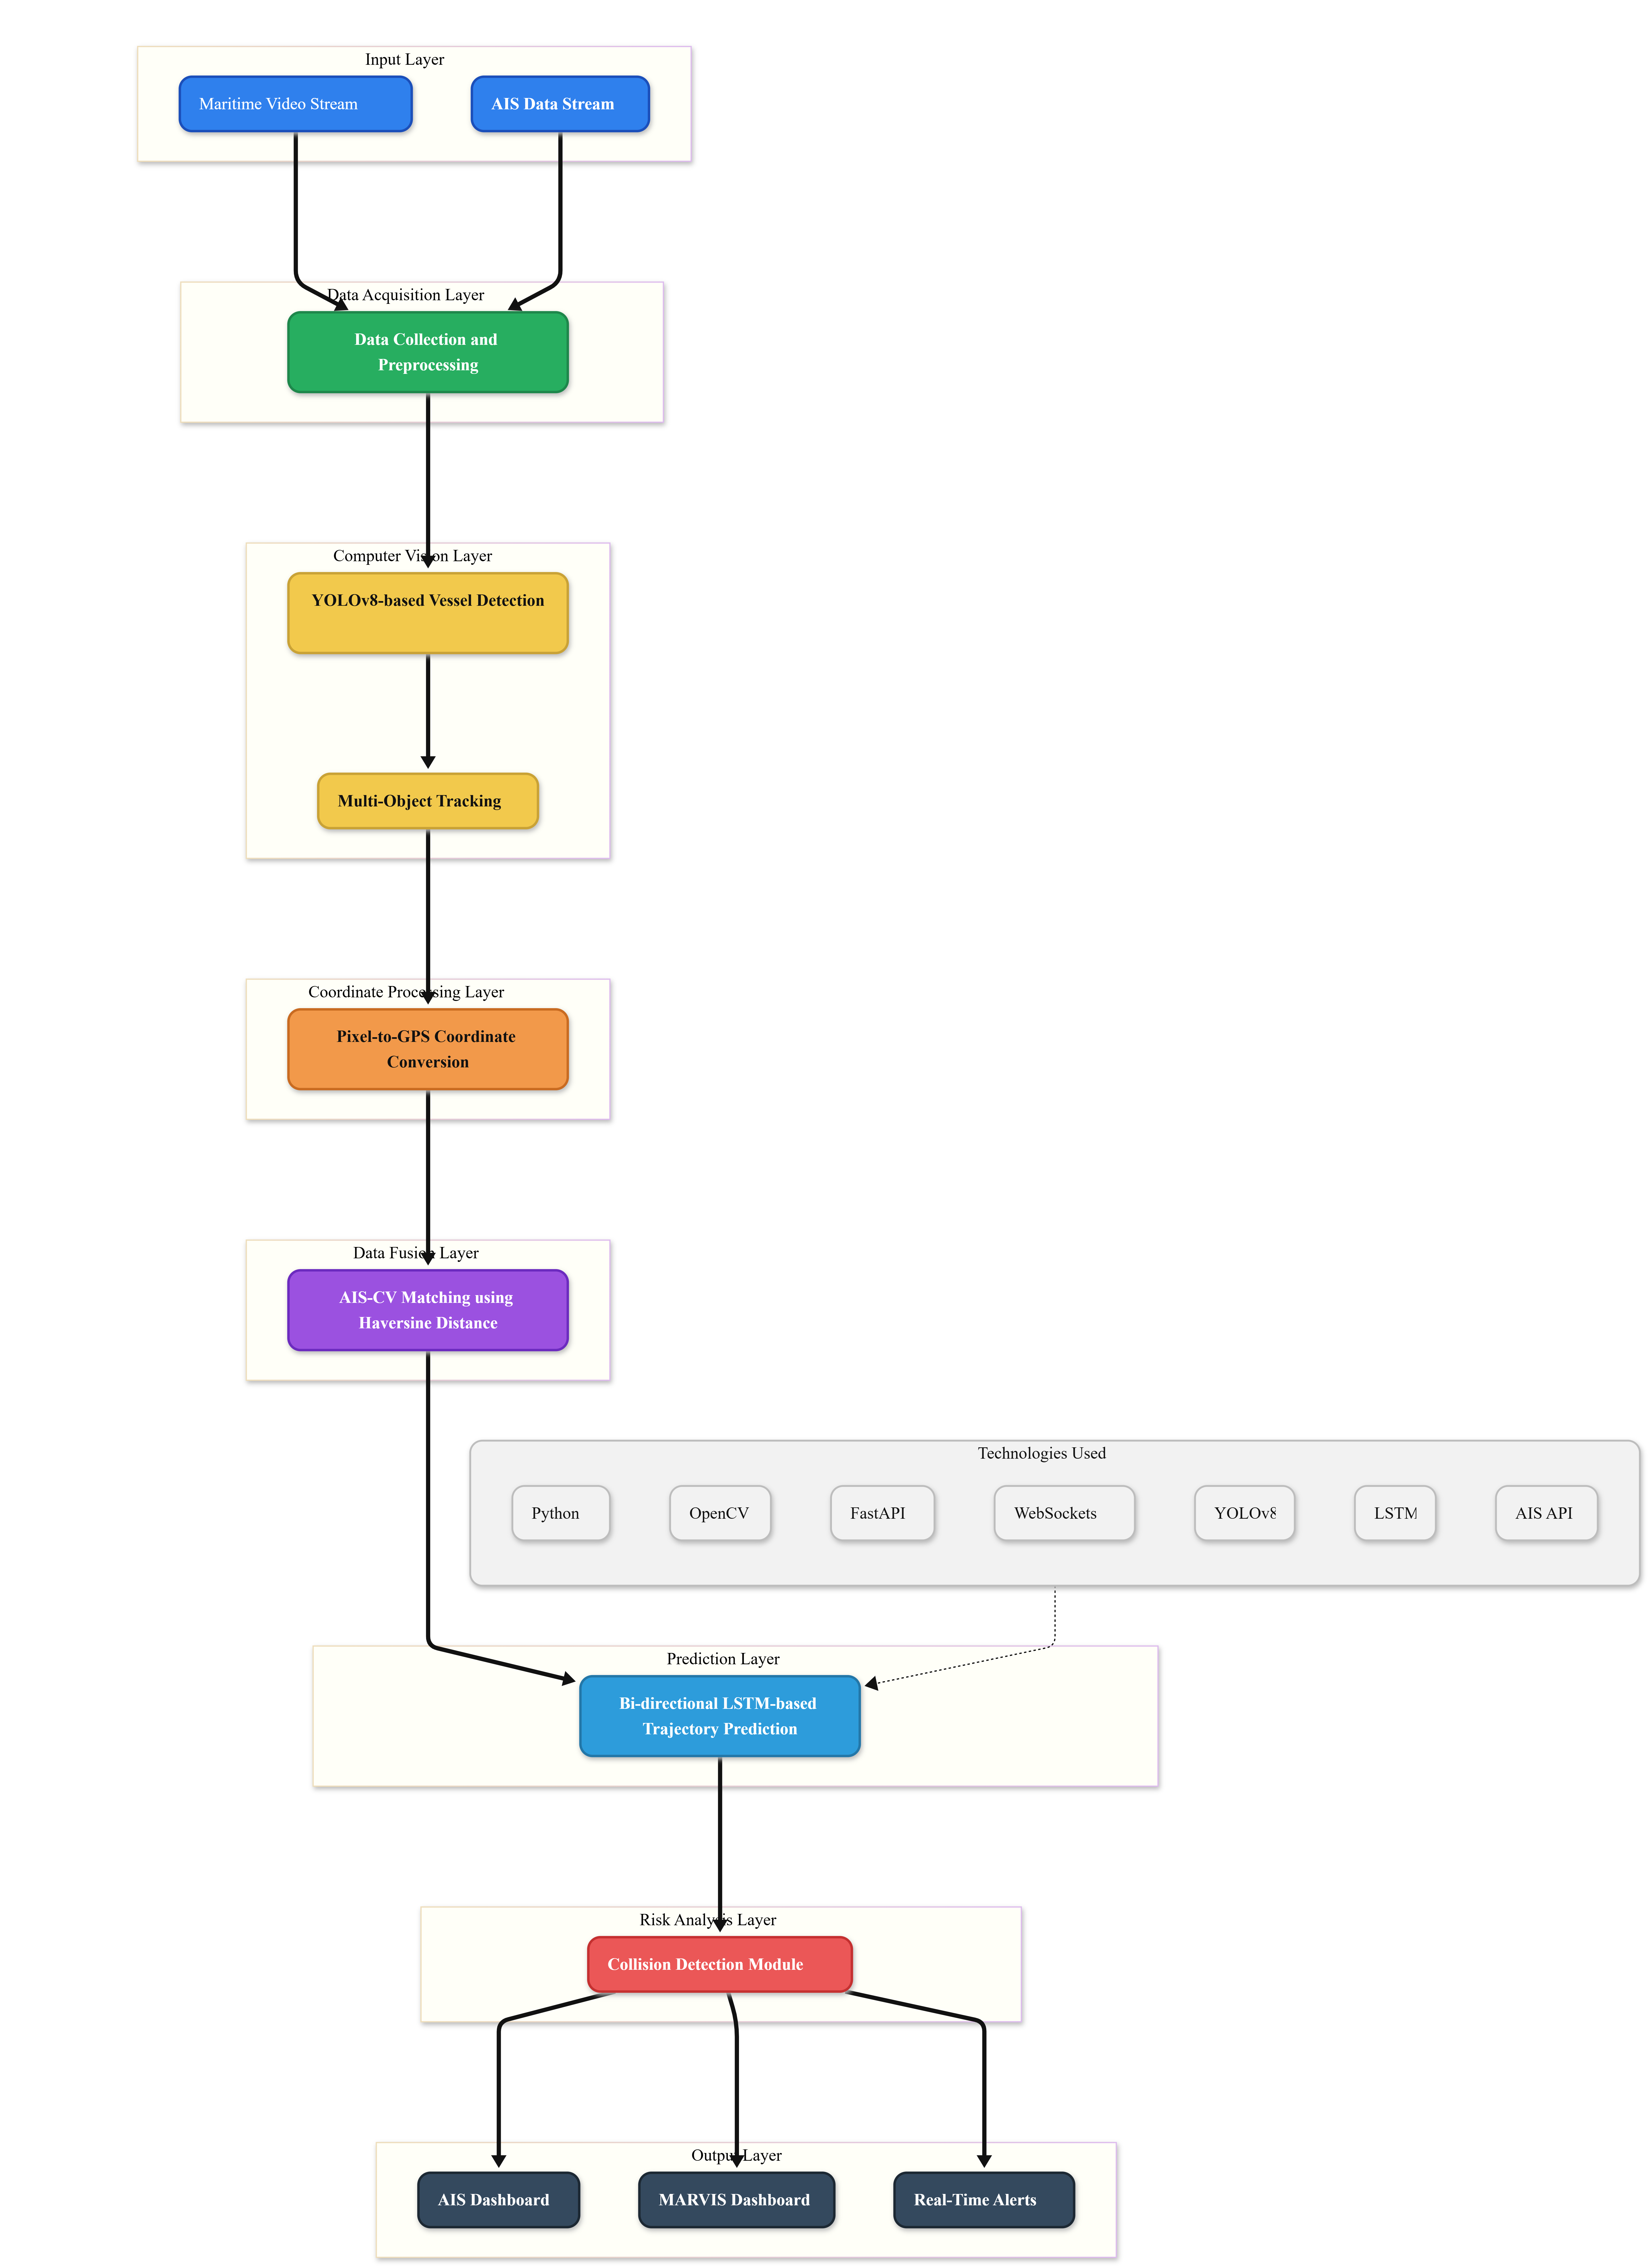
\includegraphics[width=0.95\textwidth]{Chapter3/Figures/system_architecture.png}
\caption{Overall Architecture of Proposed AI-Based Maritime Surveillance System}
\label{fig:architecture}
\end{figure}

\subsection{Specifications for the Design}
The proposed maritime surveillance system is designed to meet the following 
technical requirements. The system accepts continuous video input at a minimum 
resolution of 1280$\times$720 pixels and targets a processing throughput of up 
to 30 frames per second, ensuring real-time surveillance capability. The \gls{yolov8} 
detection module operates with a confidence threshold of 0.4 and an \gls{iou} threshold of 0.3 for \gls{nms}, balancing 
detection sensitivity against false-positive suppression. The \gls{deepocsort} tracker 
is configured with a maximum track age of 30 frames, a minimum confirmation hit 
count of 3, a detection threshold of 0.3, and cosine similarity as the distance 
metric for appearance-based \gls{reid} using the \gls{osnet} backbone.

The \gls{lstm} trajectory prediction module accepts a sequence of 50 timesteps as 
input and predicts the next 20 future positions per vessel. In the geospatial 
mapping module, pixel coordinates are transformed into geographic 
latitude--longitude pairs using a homographic transformation matrix computed via 
\texttt{cv2.findHomography} when ground-control calibration points are available, 
with a \gls{fov} linear approximation serving as the fallback. \gls{gps} positions 
derived from the pixel-to-coordinate transformation are further smoothed using a 
per-vessel Kalman filter with a constant-velocity motion model, which reduces the 
impact of detection jitter on downstream fusion and prediction. A land-mask 
post-processing stage validates all predicted vessel positions against a 
geographic water-area filter, ensuring that forecast trajectories remain within 
physically navigable regions. \gls{nvidia} \gls{cuda} acceleration is supported for real-time 
throughput. The system is implemented in Python using \gls{pytorch} as the deep learning 
framework and \gls{opencv} for video ingestion and frame-level processing.

A comprehensive pre-analysis was performed prior to the design of the system, 
involving dataset evaluation, model selection, and algorithmic benchmarking to 
ensure each component is well matched to the maritime surveillance environment.

\subsubsection{Use Case Analysis}

The use case diagram represents the interaction between users and the proposed maritime surveillance system. The major functionalities include video acquisition, vessel detection, tracking, trajectory prediction, and visualization. The diagram provides a high-level view of the system functionality and user interactions.
\begin{figure}[H]
\centering
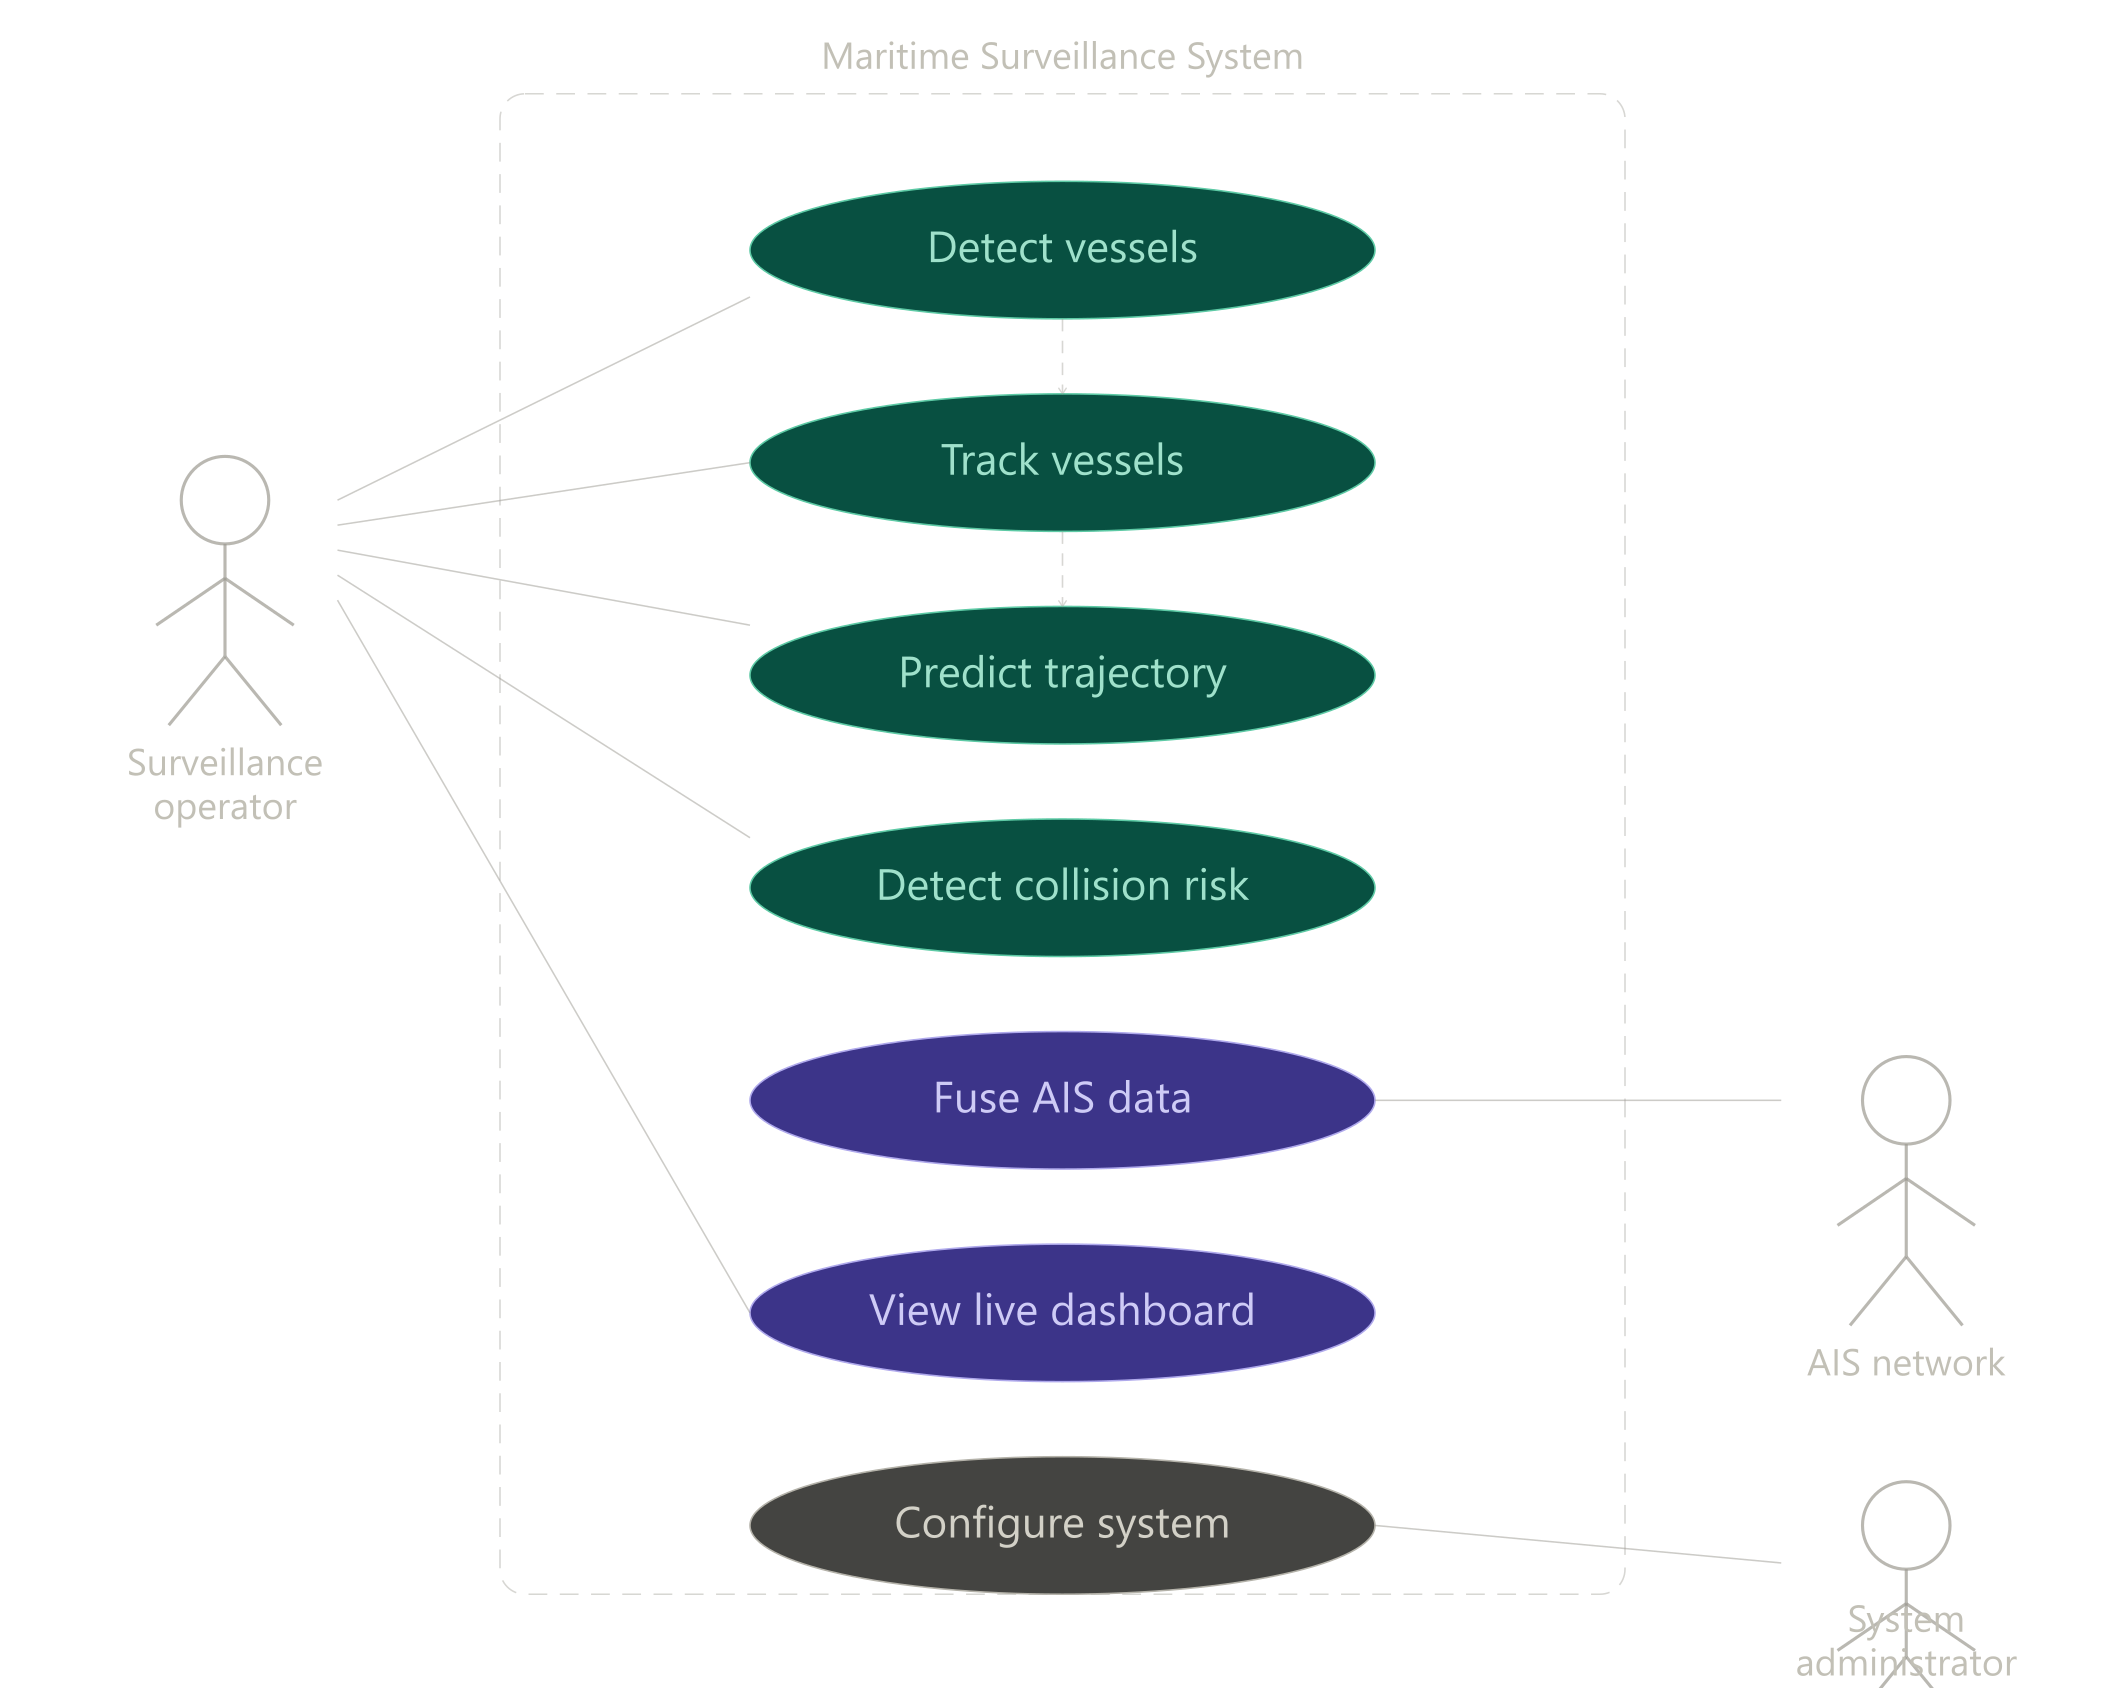
\includegraphics[width=0.95\textwidth]{Chapter3/Figures/fig3_use_case_diagram.png}
\caption{Use Case Diagram of the Maritime Surveillance System}
\label{fig:use_case}
\end{figure}

\subsection{Dataset Analysis}

The datasets used in this system serve two distinct purposes: the detection 
and fine-tuning of the \gls{yolov8} model, and the training of the \gls{lstm} trajectory 
prediction model. Each dataset was assessed for annotation quality, 
environmental diversity, vessel class distribution, and suitability for the 
maritime surveillance domain.

\subsubsection{Detection Dataset}

For vessel detection, the \textit{Kaggle Ships in Google Earth} dataset, 
accessed via the Roboflow platform (workspace: \texttt{robin-public}, project: 
\texttt{kaggle-ships-in-google-earth}, version 3), was used to fine-tune 
the \gls{yolov8} model. The dataset consists of aerial and satellite imagery of 
vessels annotated in \gls{yolo} format, with bounding boxes labelled for each vessel 
instance. Images were pre-processed and split into training, validation, and 
test partitions by the Roboflow pipeline. The dataset was selected for its 
diversity of sea states, illumination conditions, vessel scales, and occlusion 
scenarios, which are critical factors for a detection model intended to operate 
across varied real-world maritime surveillance conditions. Fine-tuning was 
performed on YOLOv8l for 70 epochs at an input resolution of 640$\times$640 
pixels using the dataset configuration file exported by Roboflow.

\subsubsection{Trajectory Prediction Dataset}

The \gls{smd} was used to train the \gls{lstm} trajectory 
prediction model. \gls{smd} is a publicly available benchmark captured using 
drone-mounted cameras over the Singapore Strait, one of the world's busiest 
maritime waterways, and provides ground-truth vessel trajectory annotations in 
the form of \texttt{TrackGT*.mat} files. Each \texttt{.mat} file contains a 
\texttt{Track} structure with per-vessel bounding boxes (\texttt{BB}) and a 
binary motion mask (\texttt{Motion}) indicating the frames in which each 
vessel is present. Trajectory centroids are extracted by computing the 
midpoint of each active bounding box:
\begin{equation}
    x_c = \frac{x_1 + x_2}{2}, \quad y_c = \frac{y_1 + y_2}{2}
    \label{eq:gps_conversion}
\end{equation}
Only trajectories with a minimum length of 50 frames are retained, ensuring 
that each sample contains sufficient history for the \gls{lstm} input window.

\subsubsection{Dataset Preprocessing}

The raw centroid sequences are processed by the \texttt{TrajectoryDataset} 
class using a sliding window of stride 1. Each window consists of 50 
consecutive timesteps as the input history and 20 subsequent timesteps as the 
prediction target. Positional coordinates are normalised by the video frame 
dimensions prior to feature construction:
\begin{equation}
    \hat{x} = \frac{x}{1920}, \quad \hat{y} = \frac{y}{1080}
    \label{eq:lat_offset}
\end{equation}
Per-frame velocity components are computed as first-order differences of the 
normalised positions:
\begin{equation}
    v_x^{(t)} = \hat{x}^{(t)} - \hat{x}^{(t-1)}, \quad 
    v_y^{(t)} = \hat{y}^{(t)} - \hat{y}^{(t-1)}
    \label{eq:haversine}
\end{equation}
The final input feature vector at each timestep is therefore 
$\mathbf{f}^{(t)} = [\hat{x}^{(t)},\; \hat{y}^{(t)},\; v_x^{(t)},\; 
v_y^{(t)}] \in \mathbb{R}^4$, giving an input tensor of shape 
$50 \times 4$ per sample. The processed dataset is split into training and 
validation sets in an 80:20 ratio using a fixed random seed of 42 for 
reproducibility. Training samples are loaded in shuffled mini-batches of 
size 32, while the validation set is evaluated in sequential order.

\subsubsection{Evaluation Protocol}

Model performance on the trajectory prediction task is quantified using two 
standard metrics. The \textit{Average Displacement Error} (\gls{ade}) measures the 
mean Euclidean distance between predicted and ground-truth positions across 
all predicted timesteps:
\begin{equation}
    \text{ADE} = \frac{1}{K} \sum_{k=1}^{K} 
    \sqrt{(\hat{x}_k - x_k)^2 + (\hat{y}_k - y_k)^2}
    \label{eq:LSTM1}
\end{equation}
The \textit{Final Displacement Error} (\gls{fde}) measures the Euclidean distance 
at the last predicted timestep only:
\begin{equation}
    \text{FDE} = \sqrt{(\hat{x}_K - x_K)^2 + (\hat{y}_K - y_K)^2}
    \label{eq:LSTM2}
\end{equation}
These metrics are computed separately for the \gls{lstm} model and for a kinematic 
linear baseline, and the percentage improvement of \gls{lstm} over the baseline is 
reported for both \gls{ade} and \gls{fde}.

\subsection{Detection Model Selection}

\gls{yolov8} was selected as the vessel detection backbone following a comparative 
evaluation of \gls{yolo}-family architectures including \gls{yolo}v5, \gls{yolo}v7, and 
\gls{yolo}v7-Tiny. The key differentiating factors in favour of \gls{yolov8} are its 
anchor-free detection head, its redesigned C2f backbone module, and its 
decoupled classification and regression branches. Anchor-free designs eliminate 
the need to predefine anchor box aspect ratios, which is particularly beneficial 
in maritime scenes where vessel aspect ratios vary significantly with viewing 
angle, distance, and vessel type. The optimised feature pyramid network in 
\gls{yolov8} improves multi-scale feature aggregation, enabling the model to detect 
both large cargo vessels occupying a large portion of the frame and small 
distant vessels spanning only a few pixels. This small-object detection 
capability is critical for the intended surveillance scenario, where vessels 
at range may occupy as few as 10$\times$10 pixels in a 1280$\times$720 frame. 
The Ultralytics \gls{yolov8} implementation additionally provides a unified Python 
\gls{api} compatible with \gls{pytorch}, facilitating integration with the downstream 
tracking and prediction pipeline. The YOLOv8n variant is used at runtime for 
detection speed, while the YOLOv8l variant was used during fine-tuning on 
the Roboflow maritime dataset.

\subsection{Tracking Algorithm Selection}

\gls{deepocsort} was selected as the multi-object tracking algorithm following 
evaluation against motion-only trackers. The fundamental limitation of 
motion-only trackers such as \gls{sort} is that identity assignment relies 
exclusively on bounding-box \gls{iou} overlap between consecutive frames. In dense 
maritime scenes where vessels travel in close proximity, cross paths, or are 
temporarily occluded by structures such as port infrastructure or other 
vessels, \gls{iou}-based matching produces frequent identity switches. \gls{deepocsort} 
addresses this by augmenting the cost matrix with an appearance similarity 
term derived from an \gls{osnet} \gls{reid} model, which embeds the visual 
appearance of each detected vessel into a descriptor vector. The combined 
cost matrix incorporates both spatial proximity and appearance consistency, 
reducing identity switches in occluded and crossing scenarios. Additionally, 
\gls{deepocsort} employs a Kalman filter per track to predict the expected bounding 
box position at the next frame, providing a robust motion prior when 
detections are temporarily absent. Tracks are confirmed after a minimum of 
3 consecutive detections and are retained for up to 30 frames without a 
matching detection before being discarded, preventing the proliferation of 
spurious track identities from transient false positives.

\subsection{Prediction Model Selection}

\gls{lstm} networks were selected for trajectory prediction in preference to Kalman 
filters and \gls{gru} variants. Kalman filters, while computationally efficient, 
operate under a linear constant-velocity motion assumption and cannot model 
the non-linear manoeuvring behaviour exhibited by maritime vessels, including 
course corrections, lane merging in traffic separation schemes, and 
speed-dependent turning arcs. \gls{gru} variants were considered as a lighter 
alternative to \gls{lstm} but were not selected because the additional gating 
complexity of \gls{lstm} — specifically the separate input, forget, and output gates 
— provides better retention of long-range temporal dependencies, which is 
necessary when a vessel's future heading is influenced by a turning manoeuvre 
that began many frames prior. The selected architecture is a \gls{seqtwo} \gls{lstm} with 
a bidirectional encoder and a soft attention mechanism, which allows the decoder 
to focus selectively on the most predictive frames in the input history rather 
than compressing the entire 50-timestep sequence into a single fixed vector. 
For vessels whose track history has not yet reached the 50-timestep threshold 
required by the \gls{lstm} input window, a kinematic fallback using linear regression 
over the available history is employed, ensuring that the system produces a 
trajectory estimate at every frame regardless of track length.

\subsubsection{Processing Pipeline Overview}

The proposed maritime surveillance system follows a structured processing pipeline that integrates maritime video streams with \gls{ais} telemetry information for intelligent vessel monitoring and prediction. Initially, video streams undergo vessel detection and object tracking, while \gls{ais} information is simultaneously processed and interpolated to improve temporal consistency. Subsequently, geographic coordinate transformation and sensor fusion mechanisms are applied to associate visual observations with \gls{ais} information.

The fused data are then processed through a filtering and feature extraction stage before being supplied to the trajectory prediction module. A \gls{bilstm} network analyses temporal movement patterns and predicts future vessel positions. The predicted outputs are further refined through land-mask constraints and subsequently utilized for visualization and collision analysis. The complete processing workflow of the proposed system is illustrated in Fig.~\ref{fig:pipeline}.

\begin{figure}[H]
\centering
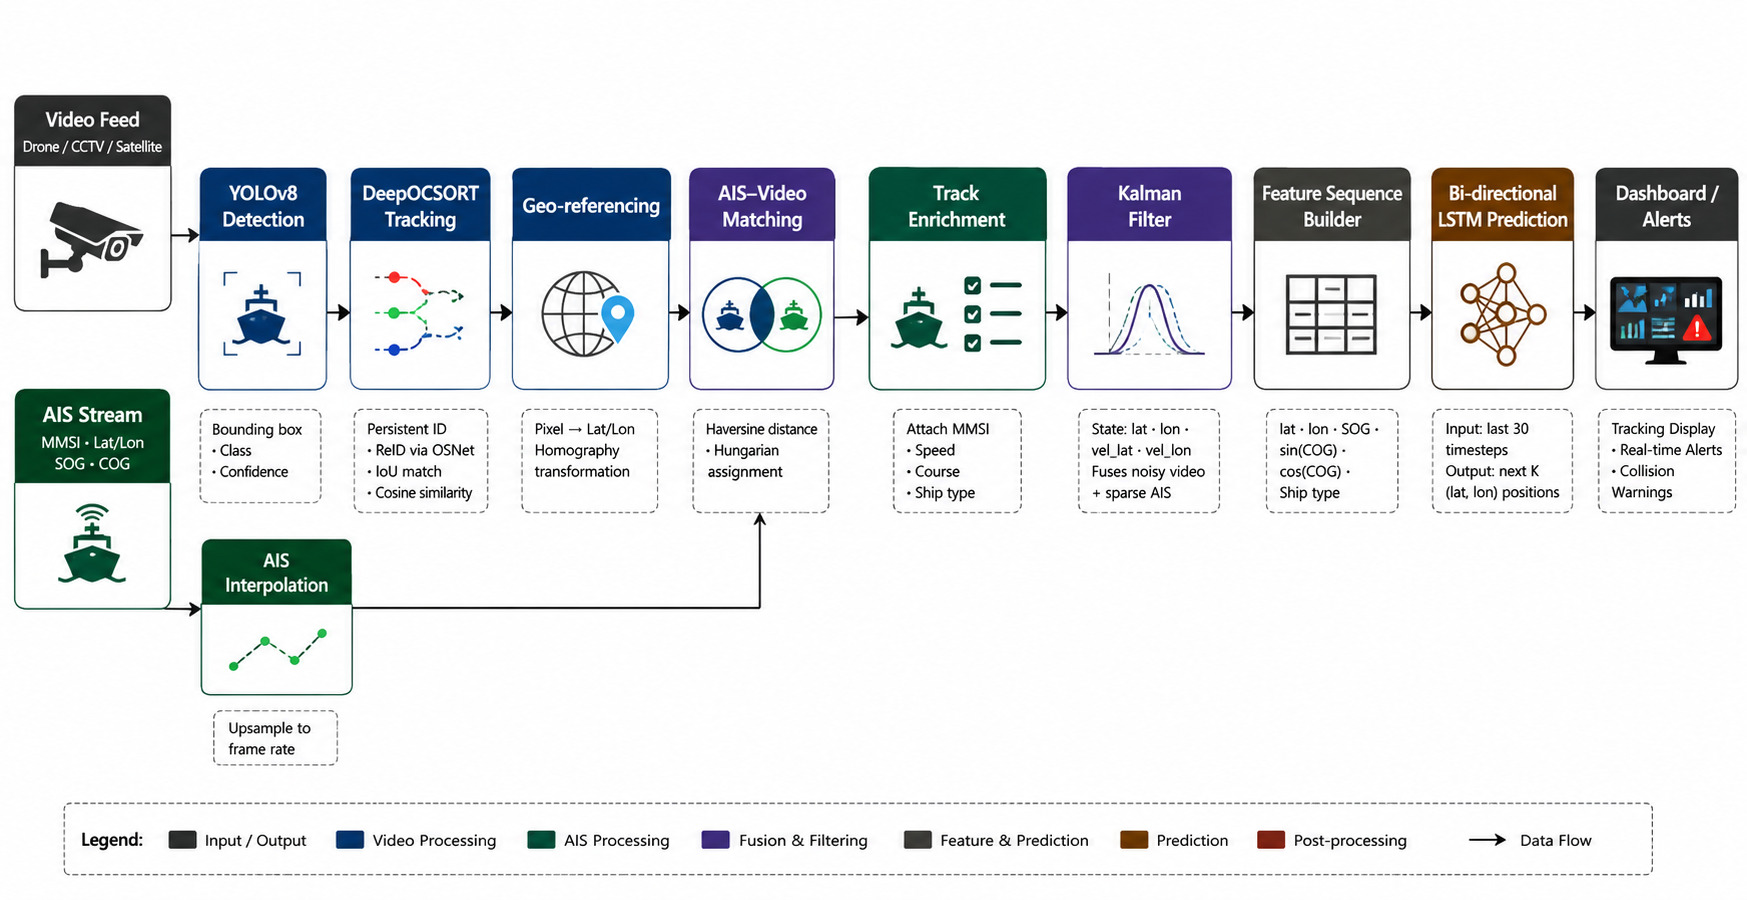
\includegraphics[width=0.85\textwidth]{Chapter3/Figures/process_pipeline.jpeg}
\caption{End-to-End Processing Pipeline of Proposed Maritime Surveillance System}
\label{fig:pipeline}
\end{figure}

\subsection{Sensor Fusion Strategy}

The complementary characteristics of video-based tracking and \gls{ais} telemetry 
present a natural opportunity for sensor fusion. Video-based tracking operates 
at frame rate, providing high-frequency positional updates, but the derived 
\gls{gps} coordinates are subject to noise introduced by pixel-to-coordinate 
projection errors and detection jitter. \gls{ais} telemetry, conversely, provides 
sparse updates at intervals of several seconds but carries precise \gls{gps} 
measurements alongside rich navigational metadata including \gls{mmsi}, vessel name, 
speed over ground (\gls{sog}), and \gls{cog}.

The fusion strategy adopted in this system is a nearest-neighbour association 
using the Haversine great-circle distance. For each camera-detected vessel 
whose pixel position has been converted to a \gls{gps} coordinate, the system queries 
the live \gls{ais} registry and computes the Haversine distance to every active \gls{ais} 
record. If the closest \gls{ais} vessel lies within the matching radius of 5.5\,km, 
the camera track is enriched with the \gls{ais} metadata: the \gls{mmsi}, vessel name, \gls{sog}, 
and \gls{cog} fields are copied into the camera detection record. Camera-detected 
vessels for which no \gls{ais} record exists within the search radius are classified 
as \textit{dark vessels} — non-cooperative targets that have either disabled 
their \gls{ais} transponder or are operating craft not required to carry \gls{ais} 
equipment. To reduce the effect of detection jitter on matching accuracy, \gls{gps} 
coordinates derived from pixel positions are smoothed using a per-vessel 
constant-velocity Kalman filter before the association step is performed.

\section{Data Flow Analysis}

The proposed maritime surveillance system processes information obtained from multiple sources and transforms it through different computational stages. Data flow analysis helps in understanding how information is exchanged between external entities, internal processing modules, and output interfaces within the system.

The system receives maritime video streams and \gls{ais} telemetry information as input. The acquired information undergoes vessel detection, tracking, coordinate transformation, data fusion, trajectory prediction, and visualization stages before generating outputs for surveillance and decision support.

\subsection{Level-0 Context Diagram}

The Level-0 Context Diagram provides a high-level representation of the interaction between external entities and the maritime surveillance system. The diagram illustrates how users, \gls{ais} data providers, and maritime video sources exchange information with the proposed system.


\begin{figure}[!htbp]
\centering
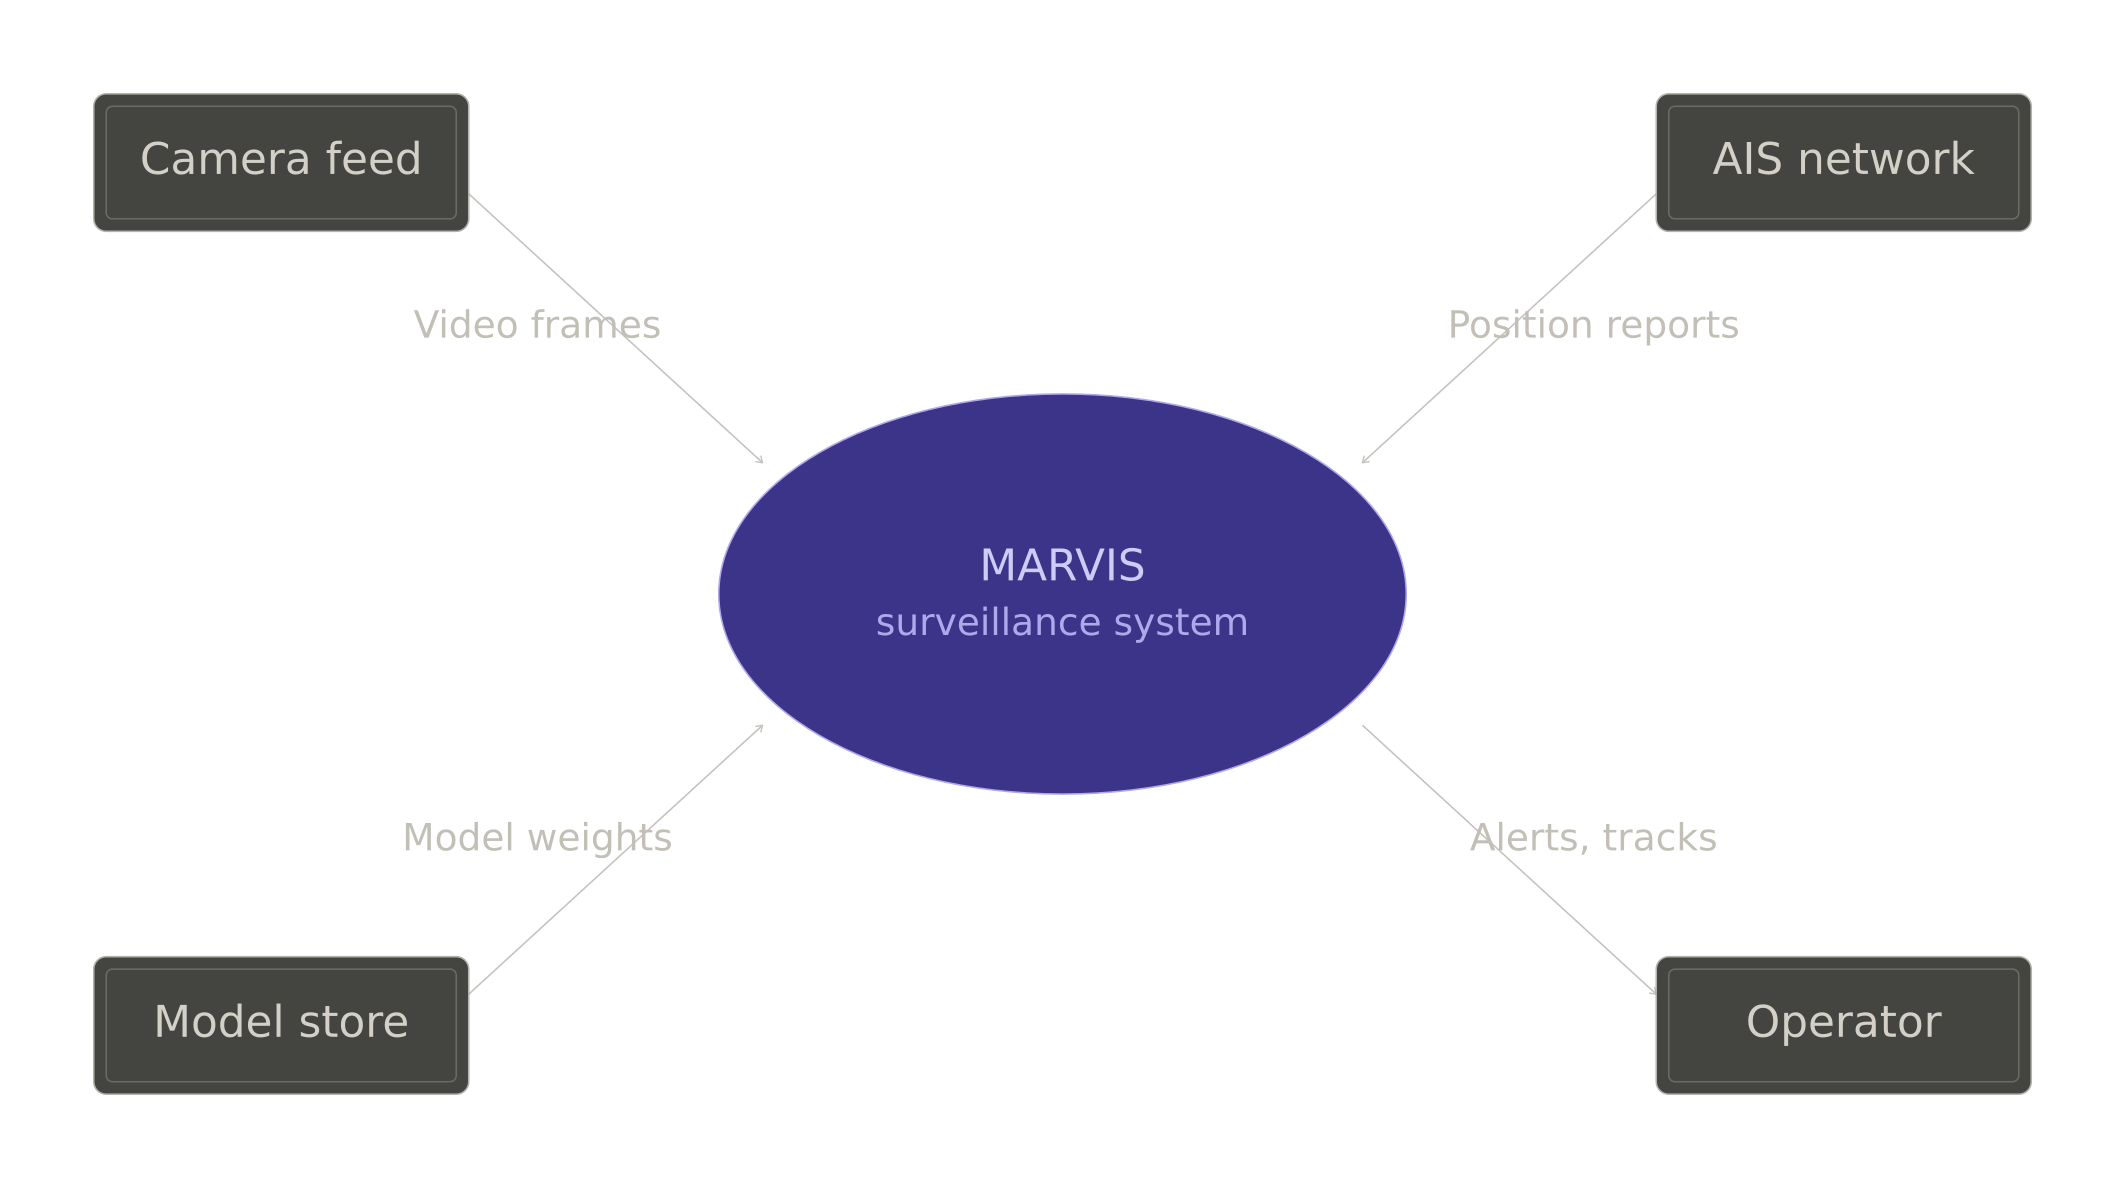
\includegraphics[width=0.95\textwidth]{Chapter3/Figures/dfd_level0_context.png}
\caption{Level-0 Context Diagram of Proposed Maritime Surveillance System}
\label{fig:dfd0}
\end{figure}

\subsection{Level-1 Data Flow Diagram}

The Level-1 Data Flow Diagram expands the internal operations of the proposed system and illustrates the flow of information across different processing modules. The workflow includes vessel detection, object tracking, coordinate transformation, \gls{ais} fusion, trajectory prediction, collision analysis, and dashboard visualization.

\begin{figure}[!htbp]
\centering
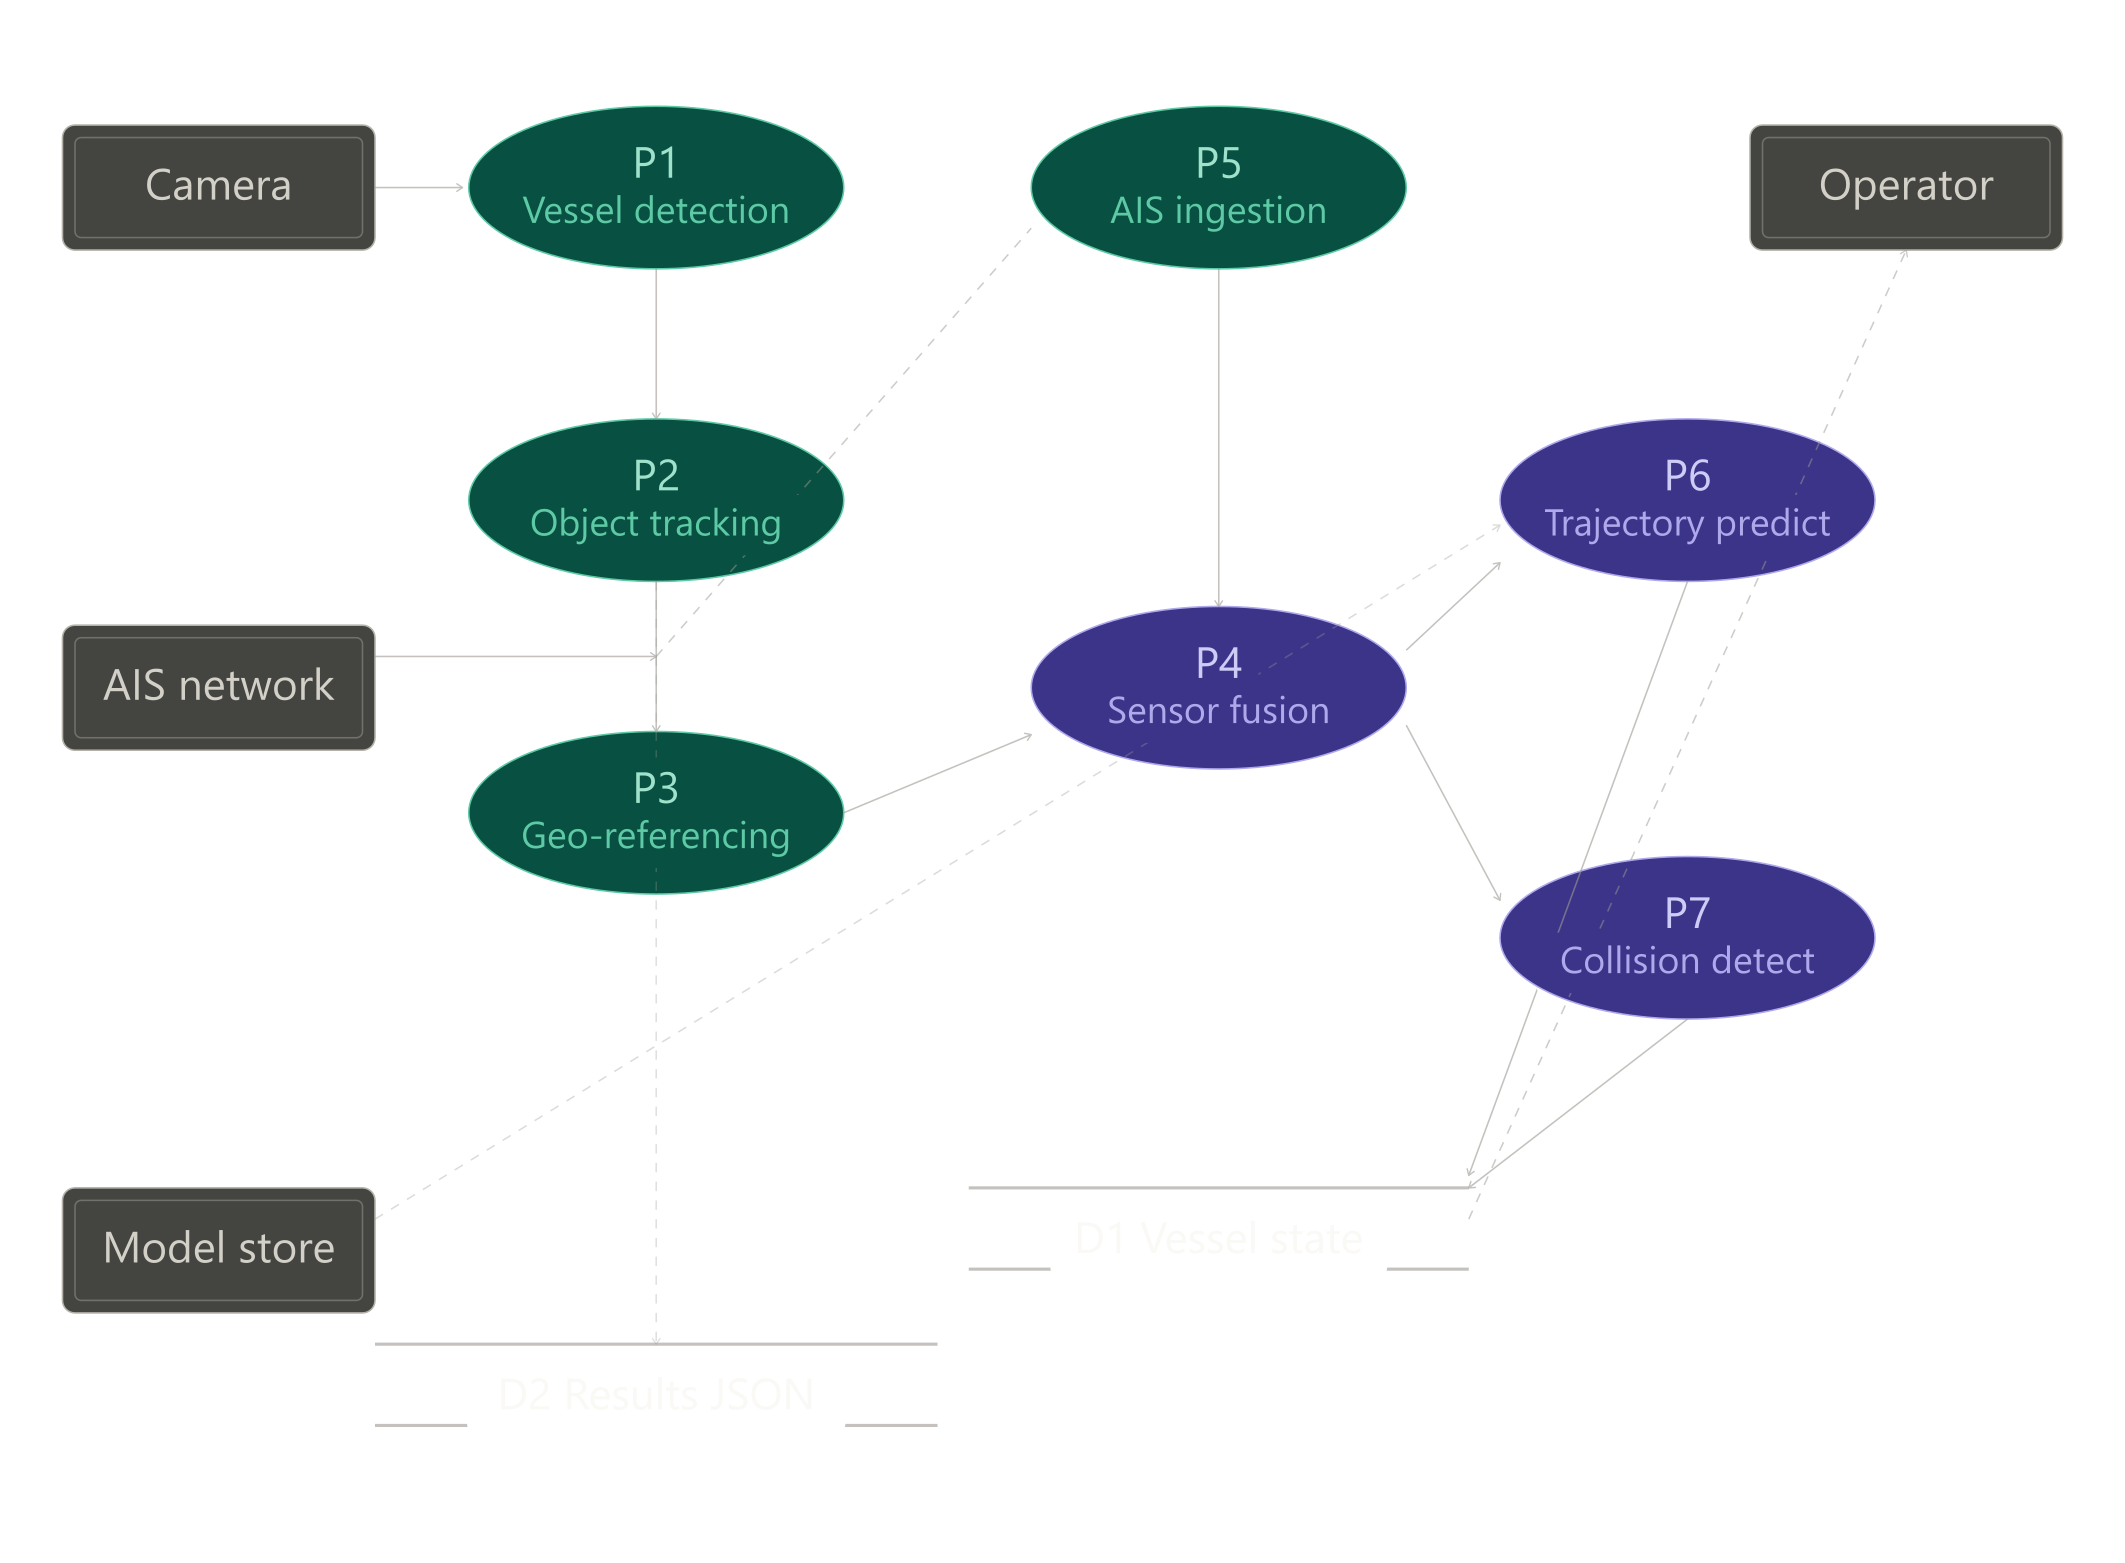
\includegraphics[width=0.95\textwidth]{Chapter3/Figures/dfd_level1_context.png}
\caption{Level-1 Data Flow Diagram of Proposed Maritime Surveillance System}
\label{fig:dfd1}
\end{figure}


\section{Module Description}

The proposed maritime surveillance system is composed of several interconnected modules that collectively enable real-time vessel monitoring, tracking, prediction, and visualization. Each module performs a dedicated task and contributes to the overall operation of the system.

\subsection{\texorpdfstring{\gls{ais}}{AIS} Data Acquisition Module}

The \gls{ais} data acquisition module is responsible for receiving and processing \gls{ais} telemetry data. The module extracts vessel identifiers, positional coordinates, speed information, and navigational parameters which are used for vessel association and monitoring.

\subsection{Video Processing Module}

The video processing module receives maritime video streams and performs frame extraction and preprocessing operations. Video frames are prepared for downstream computer vision operations.

\subsection{Vessel Detection Module}

The vessel detection module identifies ships within video frames using the \gls{yolov8} object detection model. The module generates bounding boxes around detected vessels and provides positional information for subsequent processing.

\subsection{Tracking Module}

The tracking module preserves vessel identities across consecutive frames and ensures continuity of observations. Tracking enables consistent monitoring of vessel movement throughout the surveillance period.

\subsection{Coordinate Transformation Module}

The coordinate transformation module converts image-space coordinates into geographic latitude--longitude coordinates. This conversion enables integration of visual detections with \gls{ais} telemetry data.

\subsection{Data Fusion Module}

The data fusion module combines information obtained from \gls{ais} telemetry and computer vision modules. The fusion process enriches vessel observations with navigational metadata and improves positional reliability.

\subsection{Trajectory Prediction Module}

The trajectory prediction module analyses historical movement patterns and predicts future vessel positions using a \gls{bilstm} network.

\subsection{Collision Detection Module}

The collision detection module analyses predicted trajectories and identifies possible collision scenarios among vessels operating within the monitored maritime region.

\subsection{Visualization Module}

The visualization module displays surveillance information, prediction outputs, and alert notifications through dashboard interfaces for operator monitoring and decision support.

\section{Summary}

This chapter presented a detailed account of the design and methodology 
underlying the proposed maritime surveillance system. The operational 
parameters of each module were established with explicit justification: the 
\gls{yolov8} detector was assigned a confidence threshold of 0.4 and an \gls{iou} 
threshold of 0.3 for \gls{nms}; the \gls{deepocsort} tracker was 
configured with a 90-frame history buffer, a minimum confirmation count of 3 
hits, a maximum track age of 30 frames, and a cosine similarity threshold of 
0.5 for \gls{reid}-based appearance matching; the \gls{fov} geo-referencing 
transform was anchored to the Singapore Strait camera position; the \gls{cv}-to-\gls{ais} 
fusion layer applied the Haversine nearest-neighbour method with a matching 
radius of 5.5\,km and a stale-record timeout of 300 seconds; and the \gls{seqtwo} 
\gls{lstm} predictor employed a bidirectional encoder with soft attention and a 
20-step autoregressive decoder, with kinematic linear regression as the 
fallback for tracks with fewer than 10 observations.

The pre-analysis stage evaluated candidate components across the full pipeline. 
Three object detection architectures --- Faster R-\gls{cnn}, \gls{ssdalg}, and the \gls{yolo} 
family (v5, v7, v8) --- were assessed under maritime-specific conditions 
including horizon glare, strong scale variation, and the requirement for 
real-time throughput. \gls{yolov8} was selected on the basis of its anchor-free 
regression head, enhanced feature pyramid neck, and superior small-object 
detection performance. For tracking, \gls{deepocsort} was preferred over 
motion-only trackers such as \gls{sort} and \gls{bytetrack} because its joint 
Kalman-filter--\gls{reid} association substantially reduced identity-switch events 
in occluded and crossing scenarios. For trajectory prediction, three 
candidate methods --- pure Kalman filter extrapolation, \glspl{gru}, and \gls{seqtwo} 
\glspl{lstm} --- were compared; the \gls{lstm} was chosen for its ability to model 
non-linear temporal dependencies and to focus selectively on the most 
informative history frames through its attention mechanism.

A rigorous mathematical foundation was established for each processing stage. 
The geo-referencing transform was formalised as an \gls{fov}-based linear 
approximation mapping pixel offsets from the frame centre to geographic 
latitude--longitude offsets (Equations~\ref{eq:lat_offset}--\ref{eq:gps_conversion}). 
The \gls{cv}-to-\gls{ais} spatial matching criterion was expressed using the Haversine 
great-circle distance formula 
(Equation~\ref{eq:haversine}). The \gls{lstm} architecture was formalised through 
the bidirectional encoder state update, the soft-attention weight computation, 
and the autoregressive decoder output equation 
(Equations~\ref{eq:LSTM1}--\ref{eq:LSTM2}). Together these formulations 
provide a complete theoretical account of the coordinate transformations, 
association decisions, and predictive inference steps that constitute the 
pipeline.

The two-phase pipeline architecture was then described in full, tracing the 
flow of data from raw video ingestion and live \gls{ais} stream reception through 
vessel detection, identity-preserving tracking, geo-referencing, 
nearest-neighbour \gls{ais} fusion, feature sequence construction, \gls{lstm} trajectory 
prediction, land-mask post-processing, and final output generation to the 
dashboard and results store.
		
		%Chapter 4
		\chapter{Implementation of the MARVIS System}

Transitioning a designed system into a fully operational, real-time surveillance framework demands strict integration of disparate processing modules, software libraries, and hardware resources. This chapter details how the architectural decisions outlined previously were practically executed to construct a unified pipeline capable of live vessel monitoring and trajectory forecasting. 

Rather than building the system as a monolithic application, I adopted a modular implementation strategy. Each component—ranging from video ingestion to sensor fusion—was developed, configured, and tested in isolation. This approach made it significantly easier to trace bugs and optimize performance before bringing the entire pipeline online. The following sections detail the environment configuration, data preparation, model training, and the final assembly of the functional modules.

\section{Top-Level System Implementation}

At the highest level, the implementation relies on a pipeline architecture where each stage operates independently but communicates via strictly defined data interfaces. This prevents a bottleneck in one area (such as the computationally heavy trajectory prediction) from crashing the real-time video feed. 

The framework is divided into six primary stages: video ingestion, ship detection, multi-object tracking, sensor fusion, trajectory prediction, and geospatial visualization. Figure~\ref{fig:deployment} illustrates how these modules are deployed and how data flows between them in the backend environment.

\begin{figure}[H]
\centering
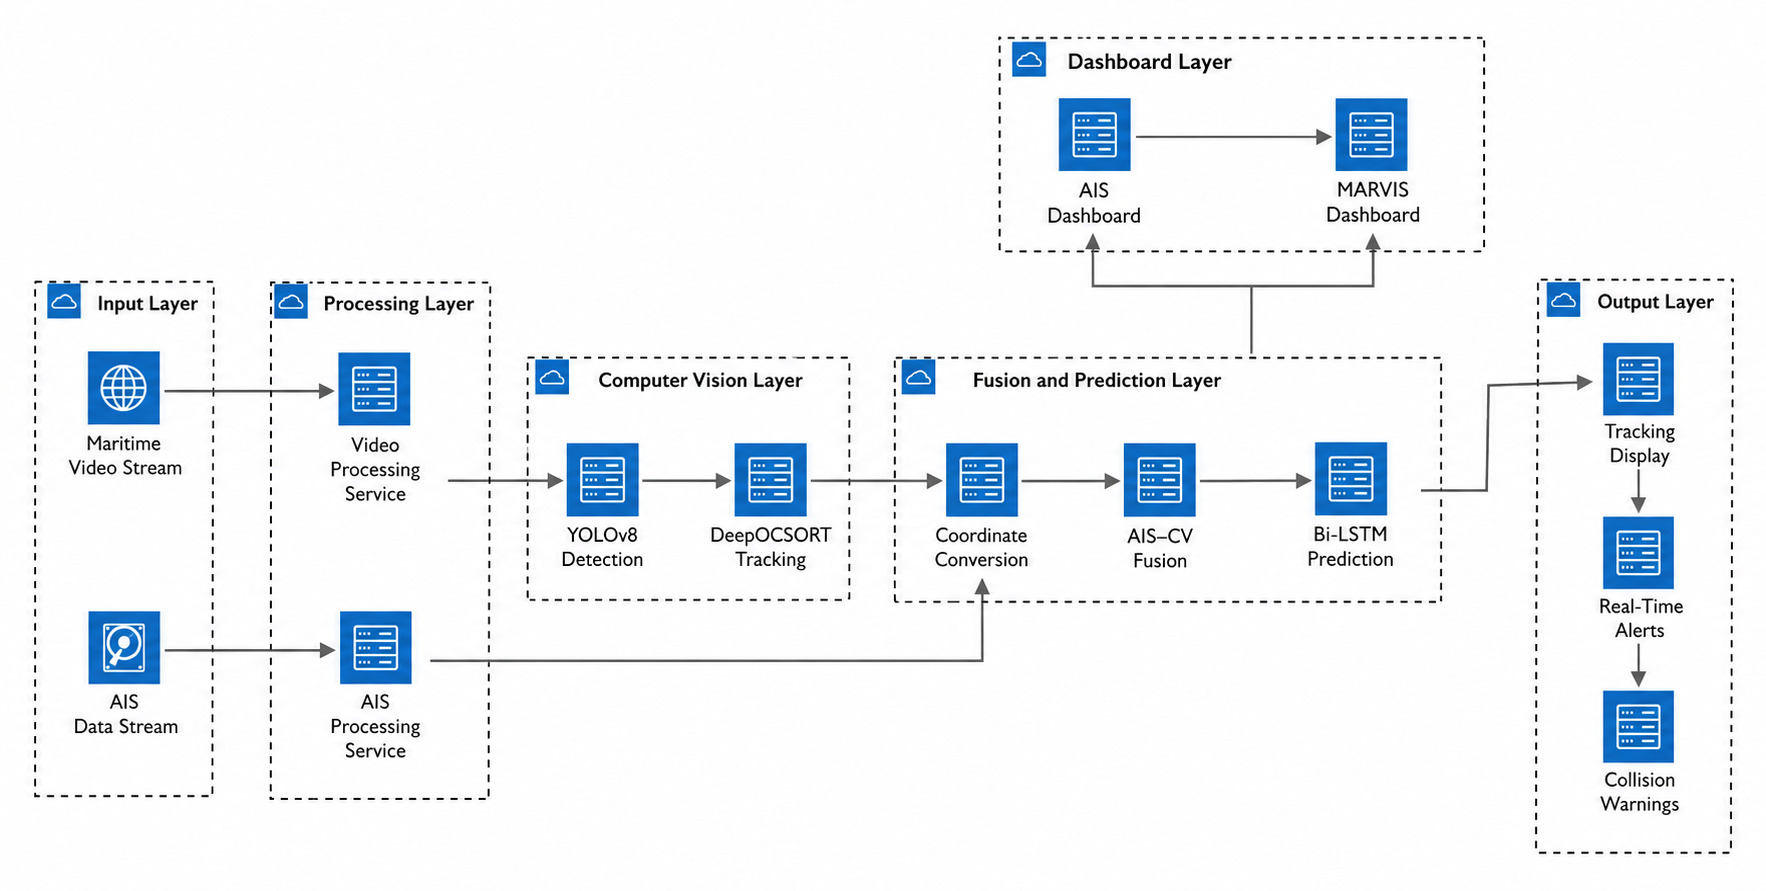
\includegraphics[width=0.95\textwidth]{Chapter4/Figures/deployment_architecture.jpeg}
\caption{Deployment and Backend Communication Architecture of Proposed Maritime Surveillance System}
\label{fig:deployment}
\end{figure}

\subsection{Development Environment Configuration}

The core logic was written in Python 3.8, selected primarily for its deep ecosystem of machine learning libraries. Deep learning operations—specifically the \gls{yolov8} detector and the \gls{lstm} forecasting network—were implemented using \gls{pytorch}. 

For the vision pipeline, \gls{opencv} handled all video ingestion, frame-by-frame extraction, and the rendering of bounding boxes onto the live feed. In the background, NumPy and Pandas managed the intermediate data structures, such as the arrays holding centroid coordinate histories and the sequence buffers required by the neural networks. Visualization was split between Matplotlib for offline analytical plotting and Folium for rendering the live, interactive geographical maps.

Crucially, the entire pipeline was deployed on an \gls{nvidia} \gls{gpu}-enabled environment utilizing \gls{cuda} acceleration. Without hardware acceleration, running simultaneous deep learning detection, appearance tracking, and sequence prediction at 30 frames per second would be computationally impossible. Primary development and debugging were conducted via Visual Studio Code and Jupyter Notebooks.

\subsection{Data Preparation and Model Training}

Before integrating the vision models into the real-time pipeline, they required extensive training. The raw maritime video data was parsed into individual frames at a fixed sampling interval, generating a robust dataset that captured diverse sea states, lighting conditions, and vessel occlusions. These frames were annotated with \gls{yolo}-formatted bounding boxes that recorded the class identifier alongside the normalized center coordinates, width, and height of every visible ship. 

To prevent overfitting, the dataset was split into training, validation, and testing partitions using a 70:20:10 ratio. During the training phase, several augmentation techniques—including horizontal flipping, mosaic augmentation, random cropping, and brightness jittering—were dynamically applied to force the model to generalize across unpredictable maritime environments.

For the detection module, \gls{yolov8} was initialized with pretrained COCO weights and then fine-tuned via transfer learning. The training process utilized a Stochastic Gradient Descent (SGD) optimizer combined with a Cosine Annealing learning rate scheduler. Early stopping was implemented, halting training once the mean Average Precision (mAP) on the validation set ceased to improve. For live inference, the model was strictly constrained by a confidence threshold of 0.5 and a \gls{nms} \gls{iou} threshold of 0.45. Any bounding box prediction falling below this confidence level is immediately discarded, ensuring that the downstream tracker isn't overwhelmed by false positives.

Following detection, the confirmed bounding boxes are passed to the \gls{deepocsort} multi-object tracking module. The tracker was configured with a maximum track age of 30 frames and requires at least 3 consecutive hits to confirm a new track. To handle identity preservation, \gls{deepocsort} utilizes an \gls{osnet} feature extractor to generate compact visual embeddings of each ship. During execution, it first attempts to match new detections to existing tracks based on spatial overlap (\gls{iou}). If that fails—often due to vessels crossing paths—it compares the \gls{osnet} embeddings using cosine similarity to successfully re-identify the ship based on its appearance. Active track coordinates are subsequently stored in a rolling buffer for motion analysis.

\subsection{Motion Estimation and Sensor Fusion}

By maintaining a historical buffer of centroid coordinates for every active track, the system can continuously calculate inter-frame motion parameters. Instantaneous speed is derived from the Euclidean distance traveled across consecutive frames, while the vessel's heading is extracted from the horizontal and vertical displacements using standard trigonometric relationships. For operator clarity, these precise angular headings are mapped to cardinal and intermediate directions before being overlaid onto the live video feed.

In parallel, the sensor fusion module ingests the live \gls{ais} telemetry stream, containing critical metadata like the \gls{mmsi}, absolute geographical coordinates, \gls{sog}, and \gls{cog}. To merge these disparate data sources, the pixel coordinates of the tracked ships are projected into geographic coordinates via a homographic transformation. The system then calculates the Haversine distance between the camera-derived coordinates and the \gls{ais} reports, employing a nearest-neighbor approach to link them. 

Once associated, the visual track is appended with the \gls{ais} metadata. However, because camera projections are inherently noisy, a Kalman filter is applied to the fused state. This filter leverages the high-frequency visual updates against the sparse but accurate \gls{ais} telemetry to produce a highly stable, real-time estimate of the vessel's actual position and velocity (Figure~\ref{fig:fusion}).

\begin{figure}[H]
\centering
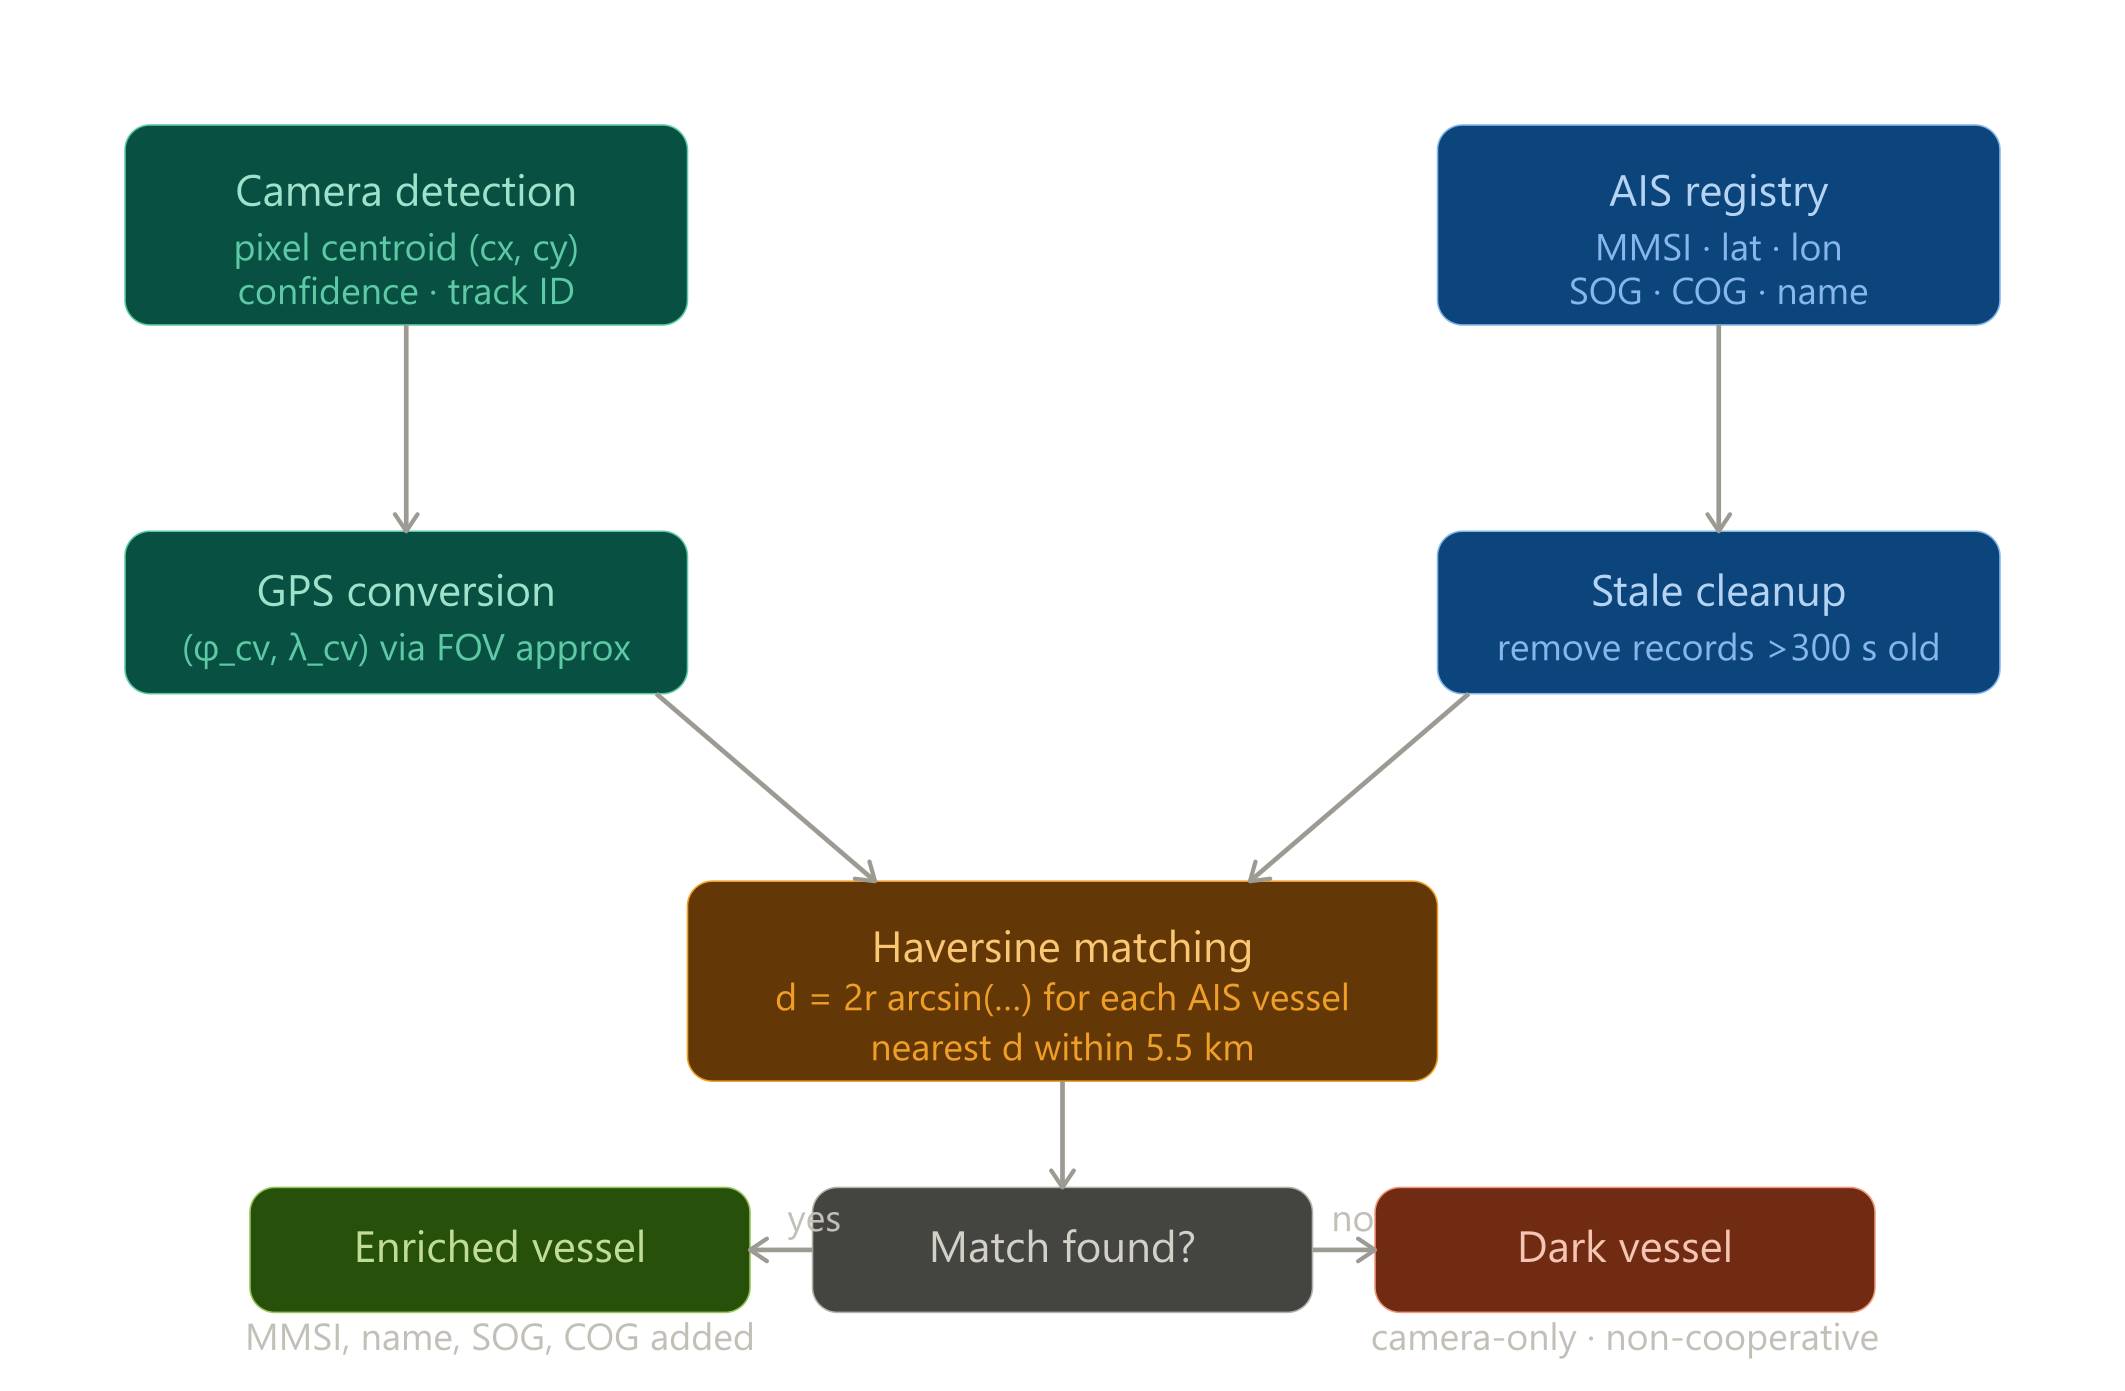
\includegraphics[width=0.95\textwidth]{Chapter4/Figures/cv_ais_fusion.png}
\caption{\gls{ais}--Computer Vision Data Fusion Process}
\label{fig:fusion}
\end{figure}

\subsection{LSTM Trajectory Prediction}

With a stable sequence of historical positions established, the data is routed to the trajectory prediction module. Because vessel movement is sequential and influenced by past maneuvers, an \gls{lstm} network was chosen over simpler regression models to capture these complex temporal dependencies.

The architecture comprises two stacked \gls{lstm} layers feeding into a fully connected output layer (Figure~\ref{fig:lstm}). The input at each timestep is a feature vector containing the vessel's latitude, longitude, \gls{sog}, sine and cosine encodings of the \gls{cog}, and a categorical vessel-type identifier. The network was trained on historical tracking data using \gls{mse} as the loss metric, optimized via the Adam algorithm. 

At runtime, the system slices the Kalman-filtered track history into fixed-length temporal windows and passes them through the trained model to forecast future coordinates. However, newly detected ships often lack sufficient historical data to fill the \gls{lstm}'s required input window. To prevent the pipeline from stalling, a kinematic linear regression fallback immediately takes over for these short-duration tracks, ensuring that the system always provides a predictive output regardless of track maturity.

\begin{figure}[H]
\centering
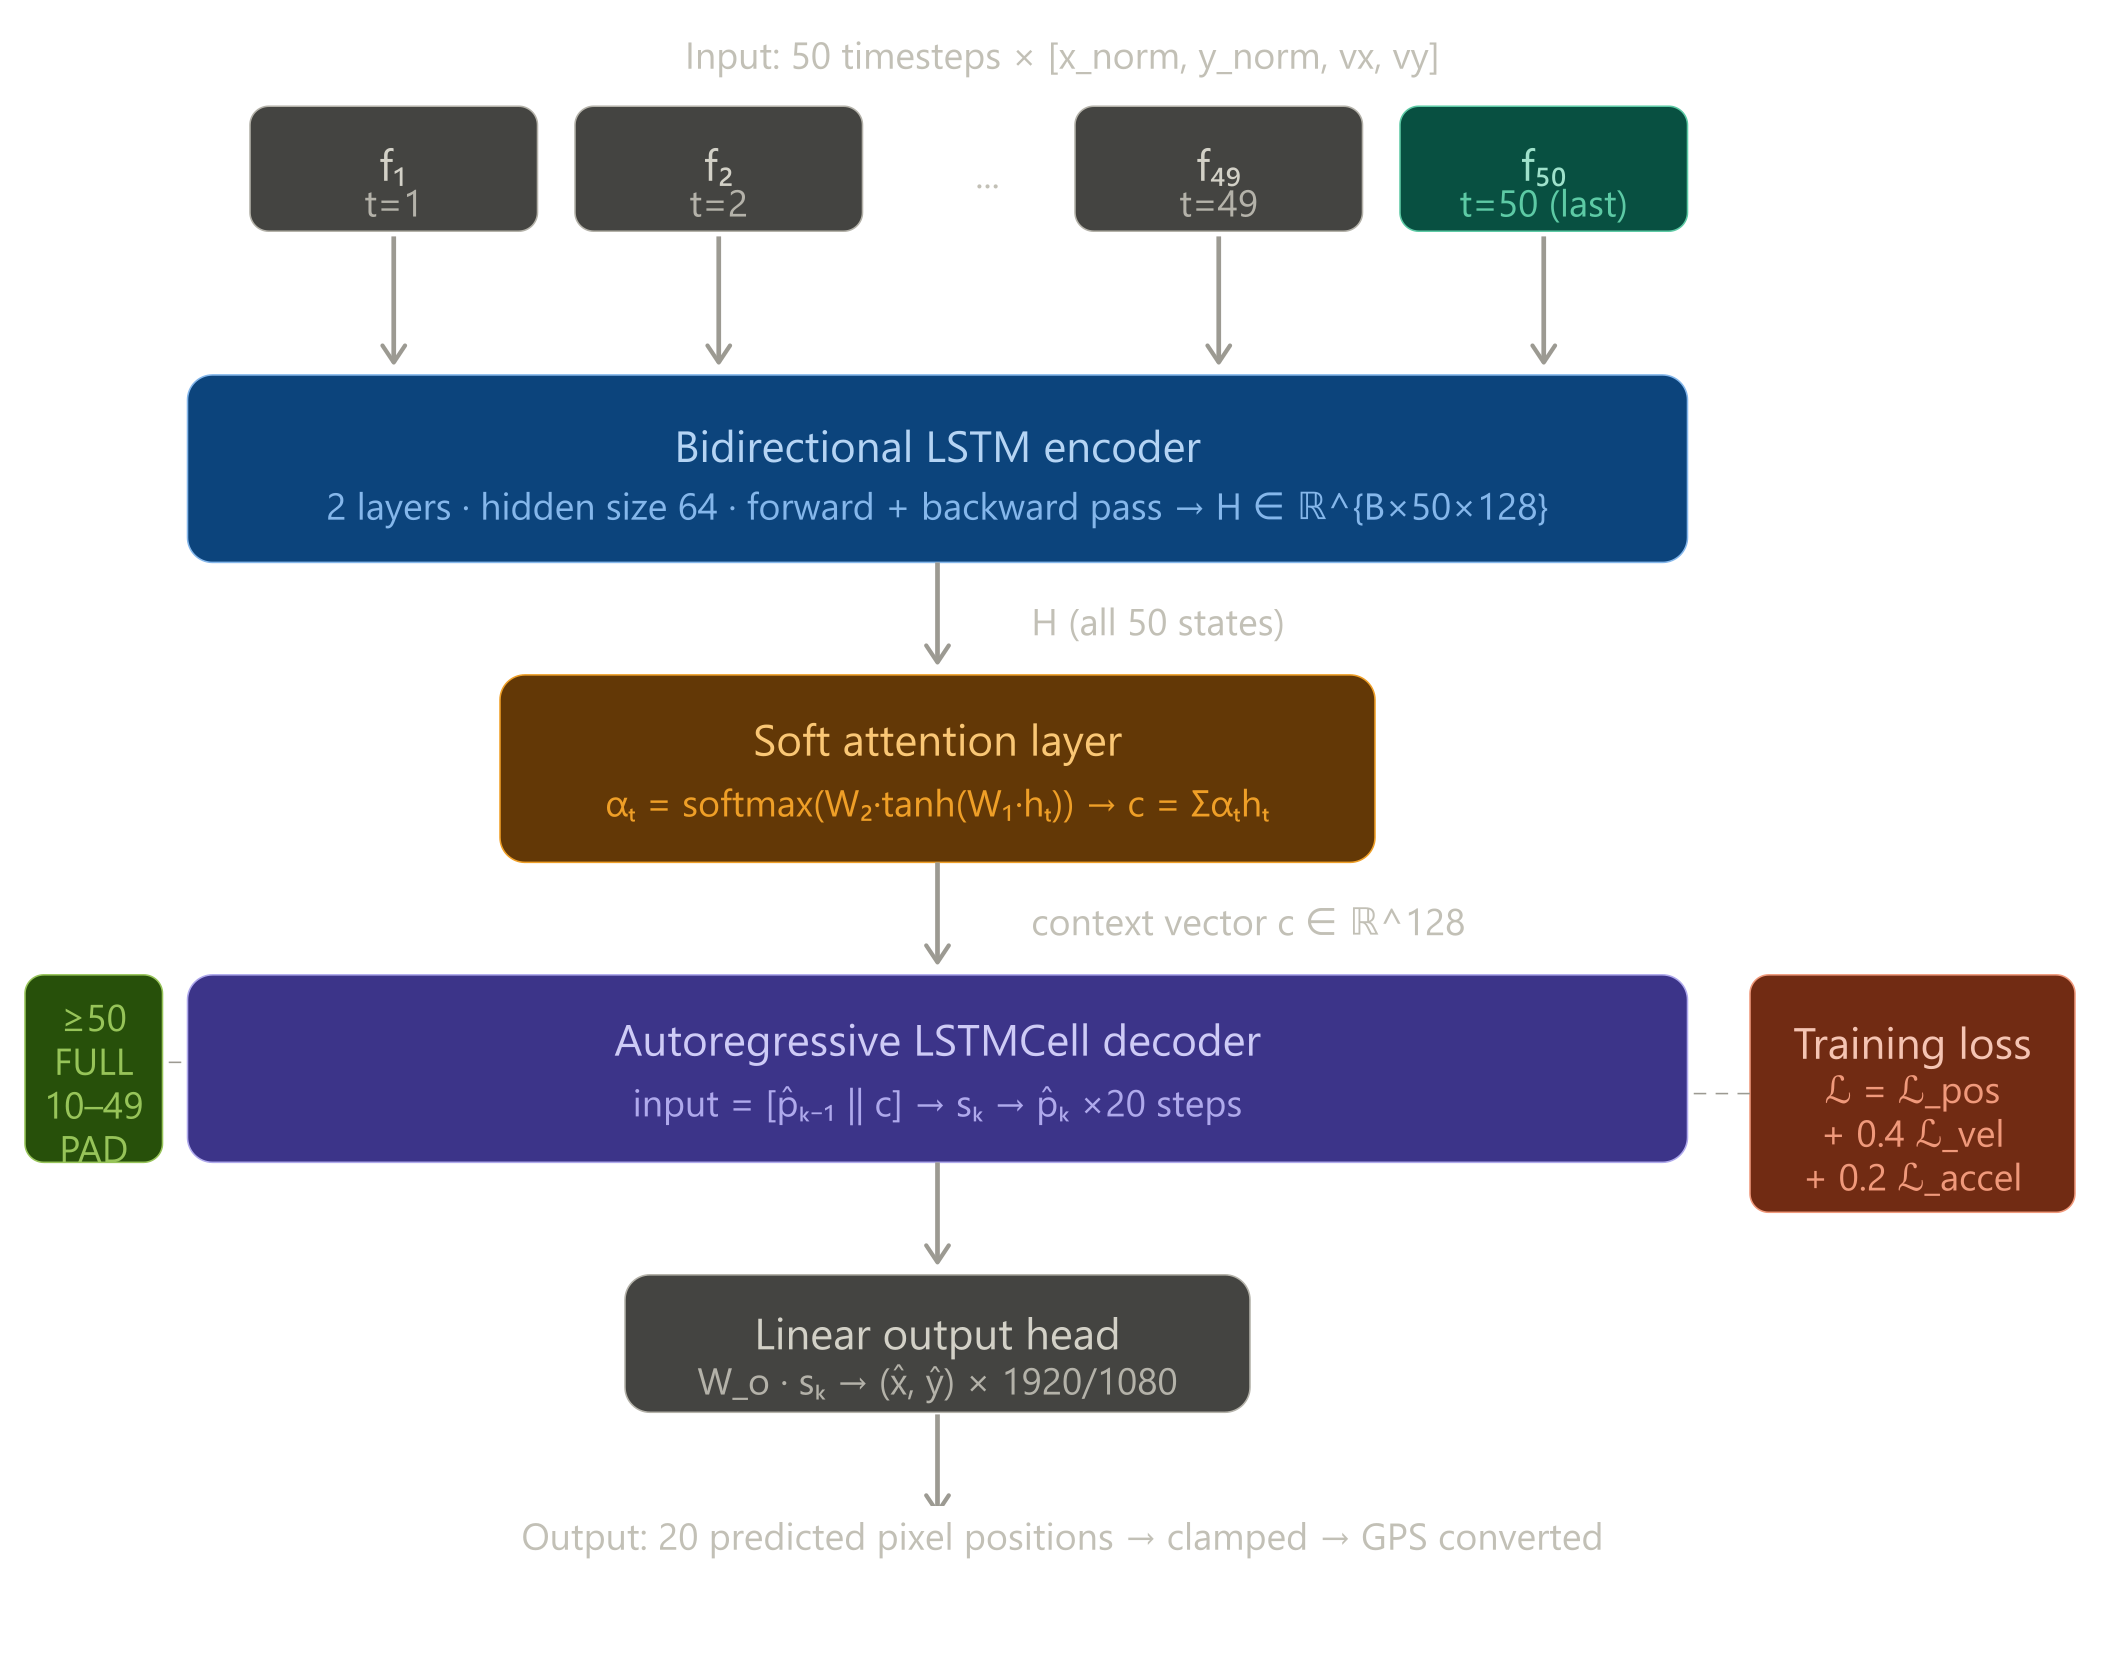
\includegraphics[width=0.90\textwidth]{Chapter4/Figures/lstm_architecture.png}
\caption{\gls{bilstm} Architecture for Vessel Trajectory Prediction}
\label{fig:lstm}
\end{figure}

\subsection{Geospatial Validation and Visualization}

Before the predicted trajectories are displayed to the user, they must pass through a land mask filter. This post-processing mechanism checks every forecasted coordinate against a global land-water topological map. If an \gls{lstm} prediction inadvertently routes a ship across a landmass—a common anomaly when predicting tight turns near coastlines—the filter intervenes, snapping the coordinate back to the nearest navigable water region. This guarantees physical realism in the system's output.

The finalized data is pushed to a dual-output visualization system. Using \gls{opencv}, bounding boxes, tracking IDs, speed annotations, and predicted paths are rendered directly onto the raw video feed for immediate visual confirmation. Concurrently, the geographical data is pushed to an interactive, Folium-based dashboard (Figure~\ref{fig:dashboard}). This web interface plots the live locations and forecasted trajectories on a global map, providing operators with comprehensive, real-time situational awareness.

\begin{figure}[H]
\centering
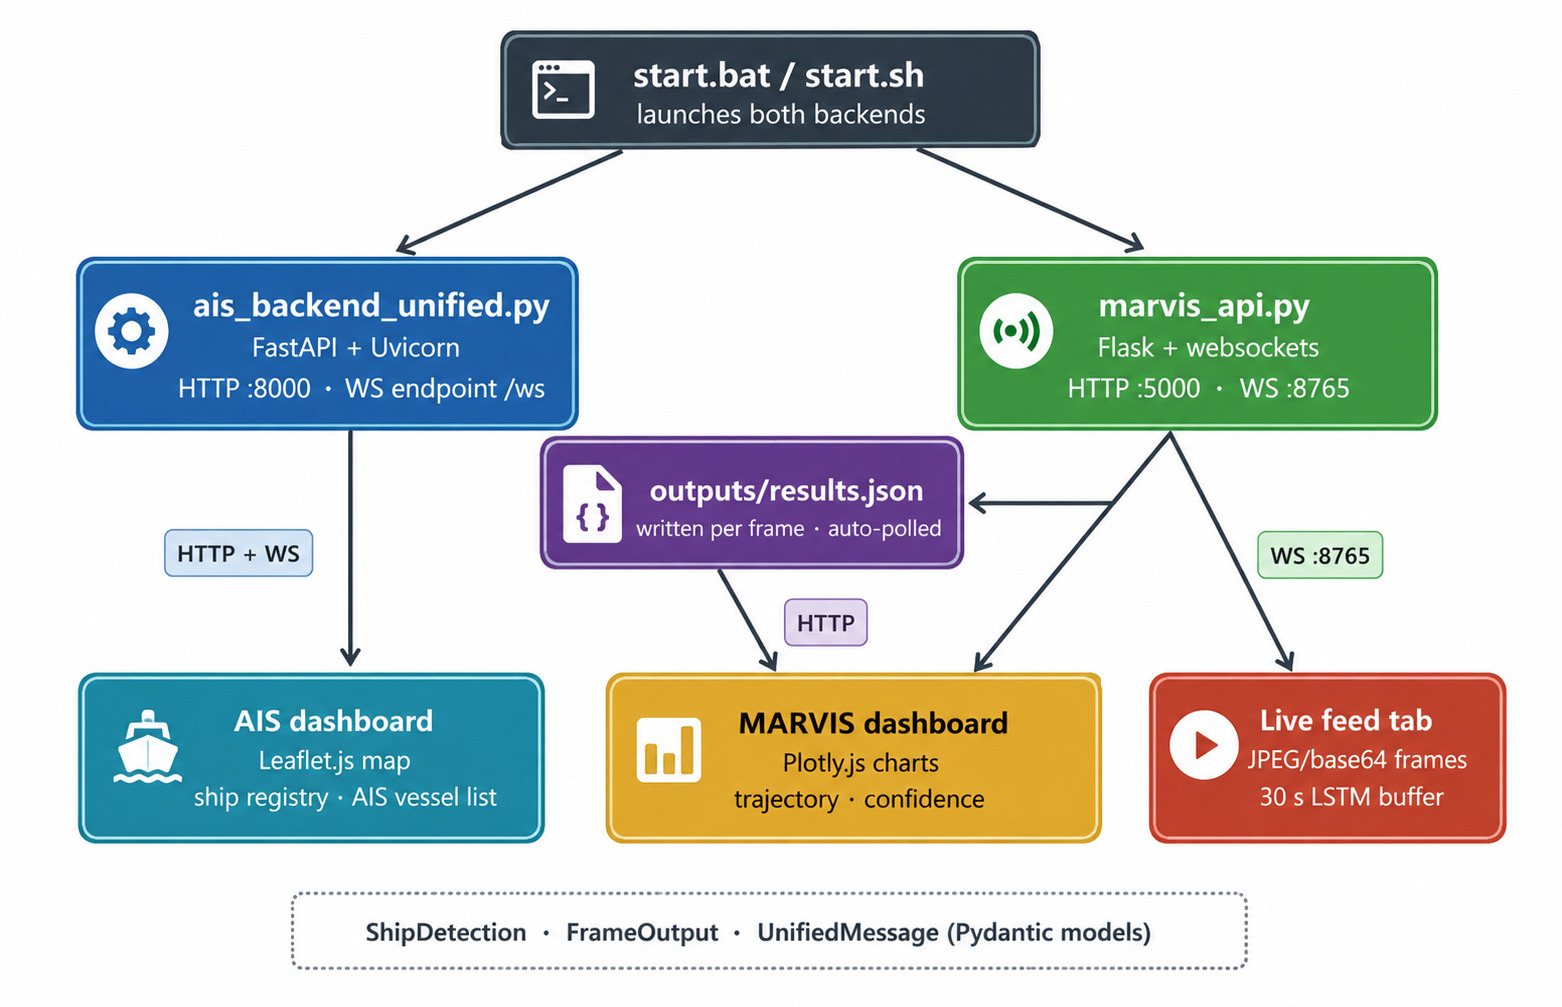
\includegraphics[width=0.95\textwidth]{Chapter4/Figures/dashboard_architecture.jpeg}
\caption{Dashboard Communication and Visualization Architecture}
\label{fig:dashboard}
\end{figure}

\section{Summary}

This chapter demonstrated how the theoretical designs from Chapter 3 were practically executed to build a functional, real-time surveillance pipeline. By establishing a \gls{cuda}-accelerated environment leveraging Python, \gls{pytorch}, and \gls{opencv}, the system successfully handles computationally intense deep learning tasks without sacrificing frame rate.

The data preparation phase established a robust 70:20:10 dataset used to fine-tune the \gls{yolov8} detector, which was seamlessly integrated with the \gls{deepocsort} tracker via \gls{osnet} appearance embeddings. By calculating inter-frame motion parameters and projecting them geographically, the pipeline successfully fuses live visual observations with \gls{ais} telemetry using Haversine nearest-neighbor matching and Kalman filtering. 

Finally, the implementation of the stacked \gls{lstm} network—supported by a kinematic regression fallback for new tracks and a land-mask filter for physical validation—ensures that the system generates highly accurate trajectory forecasts. These insights are ultimately routed to interactive \gls{opencv} and Folium dashboards, resulting in a cohesive, end-to-end framework whose performance metrics will be rigorously evaluated in the following chapter.

		
		%Chapter 5
		% -----------------------------------------------------------------------------
% CHAPTER 5 — RESULTS AND DISCUSSIONS
% -----------------------------------------------------------------------------

\chapter{Results and Discussions}

To determine the practical viability of the MARVIS framework, I evaluated the performance of its four primary processing stages: vessel detection, multi-object tracking, trajectory prediction, and collision risk detection. I assessed each module independently using standard quantitative metrics against test sequences from the Singapore Maritime Dataset (\gls{smd}). Following these individual assessments, I benchmarked the fully integrated pipeline to confirm whether it could genuinely sustain real-time throughput. 

In this chapter, I discuss the experimental setup and detail the quantitative results. I also contrast the \gls{lstm} trajectory predictor against a standard kinematic baseline and compare the overall performance of this system against recent literature in the maritime surveillance domain.

% -----------------------------------------------------------------------------
\section{Experimental Setup}
% -----------------------------------------------------------------------------

I conducted all experiments in a strictly controlled hardware and software environment to guarantee reproducible results. To support the computational demands of real-time deep learning inference, the implementation relied heavily on \gls{gpu} acceleration. Table~\ref{c5:tab:hardware} details the specific libraries and hardware configurations used during testing.

\begin{table}[H]
\centering
\caption{Hardware and Software Configuration Used for Experimental Evaluation}
\label{c5:tab:hardware}
\begin{tabular}{|p{0.34\textwidth}|p{0.34\textwidth}|}
\hline
\textbf{Component} & \textbf{Specification}\\
\hline
Operating System & Windows 11 / Ubuntu 22.04\\
Processor & Intel Core i5 12th gen / AMD Ryzen 7\\
\gls{gpu} & \gls{nvidia} \gls{gpu} with \gls{cuda} support\\
\gls{ram} & 8 GB\\
Python Version & 3.10\\
\gls{pytorch} Version & 2.2.0\\
\gls{cuda} Version & 11.8\\
\gls{opencv} Version & 4.9.0\\
Ultralytics \gls{yolov8} & v8.0\\
\gls{deepocsort} (boxmot) & v10.0\\
Evaluation Dataset & \gls{smd} v1.0\\
\hline
\end{tabular}
\end{table}

Beyond the hardware setup, I locked down several system-level parameters across all evaluation runs to prevent unintentional variations in the output. Table~\ref{c5:tab:parameters} lists the critical thresholds and tracking parameters applied during the experiments.

\begin{table}[H]
\centering
\caption{System Parameters Used During Experimental Evaluation}
\label{c5:tab:parameters}
\begin{tabular}{|p{0.34\textwidth}|p{0.34\textwidth}|}
\hline
\textbf{Parameter} & \textbf{Value}\\
\hline
Detection confidence threshold & 0.4\\
\gls{iou} threshold (\gls{nms}) & 0.3\\
Track maximum age & 30 frames\\
Track minimum hits & 3 frames\\
\gls{lstm} input sequence length & 50 timesteps\\
\gls{lstm} prediction horizon & 20 timesteps\\
Training batch size & 32\\
Training epochs & 100\\
\gls{ais} matching radius & 5.5 km\\
\gls{cpa} critical alert threshold & 50 m\\
Average input resolution & 1280$\times$720\\
Target processing speed & 30 \gls{fps}\\
\hline
\end{tabular}
\end{table}

% -----------------------------------------------------------------------------
\section{Experimental Results}
% -----------------------------------------------------------------------------

\subsection{\texorpdfstring{\gls{lstm}}{LSTM} Training Convergence}

I trained the \gls{bilstm} trajectory model for up to 100 epochs, utilizing Mean Squared Error (\gls{mse}) to penalize deviations between the predicted paths and the actual ground truth. To optimize the network weights, I used the Adam optimizer with a learning rate of 0.001 and a batch size of 32. Crucially, I implemented early stopping to prevent the model from simply memorizing the training set, thereby improving its ability to generalize to new data.

Figure~\ref{fig:c5:loss} plots the training and validation losses over time.

\begin{figure}[H]
\centering
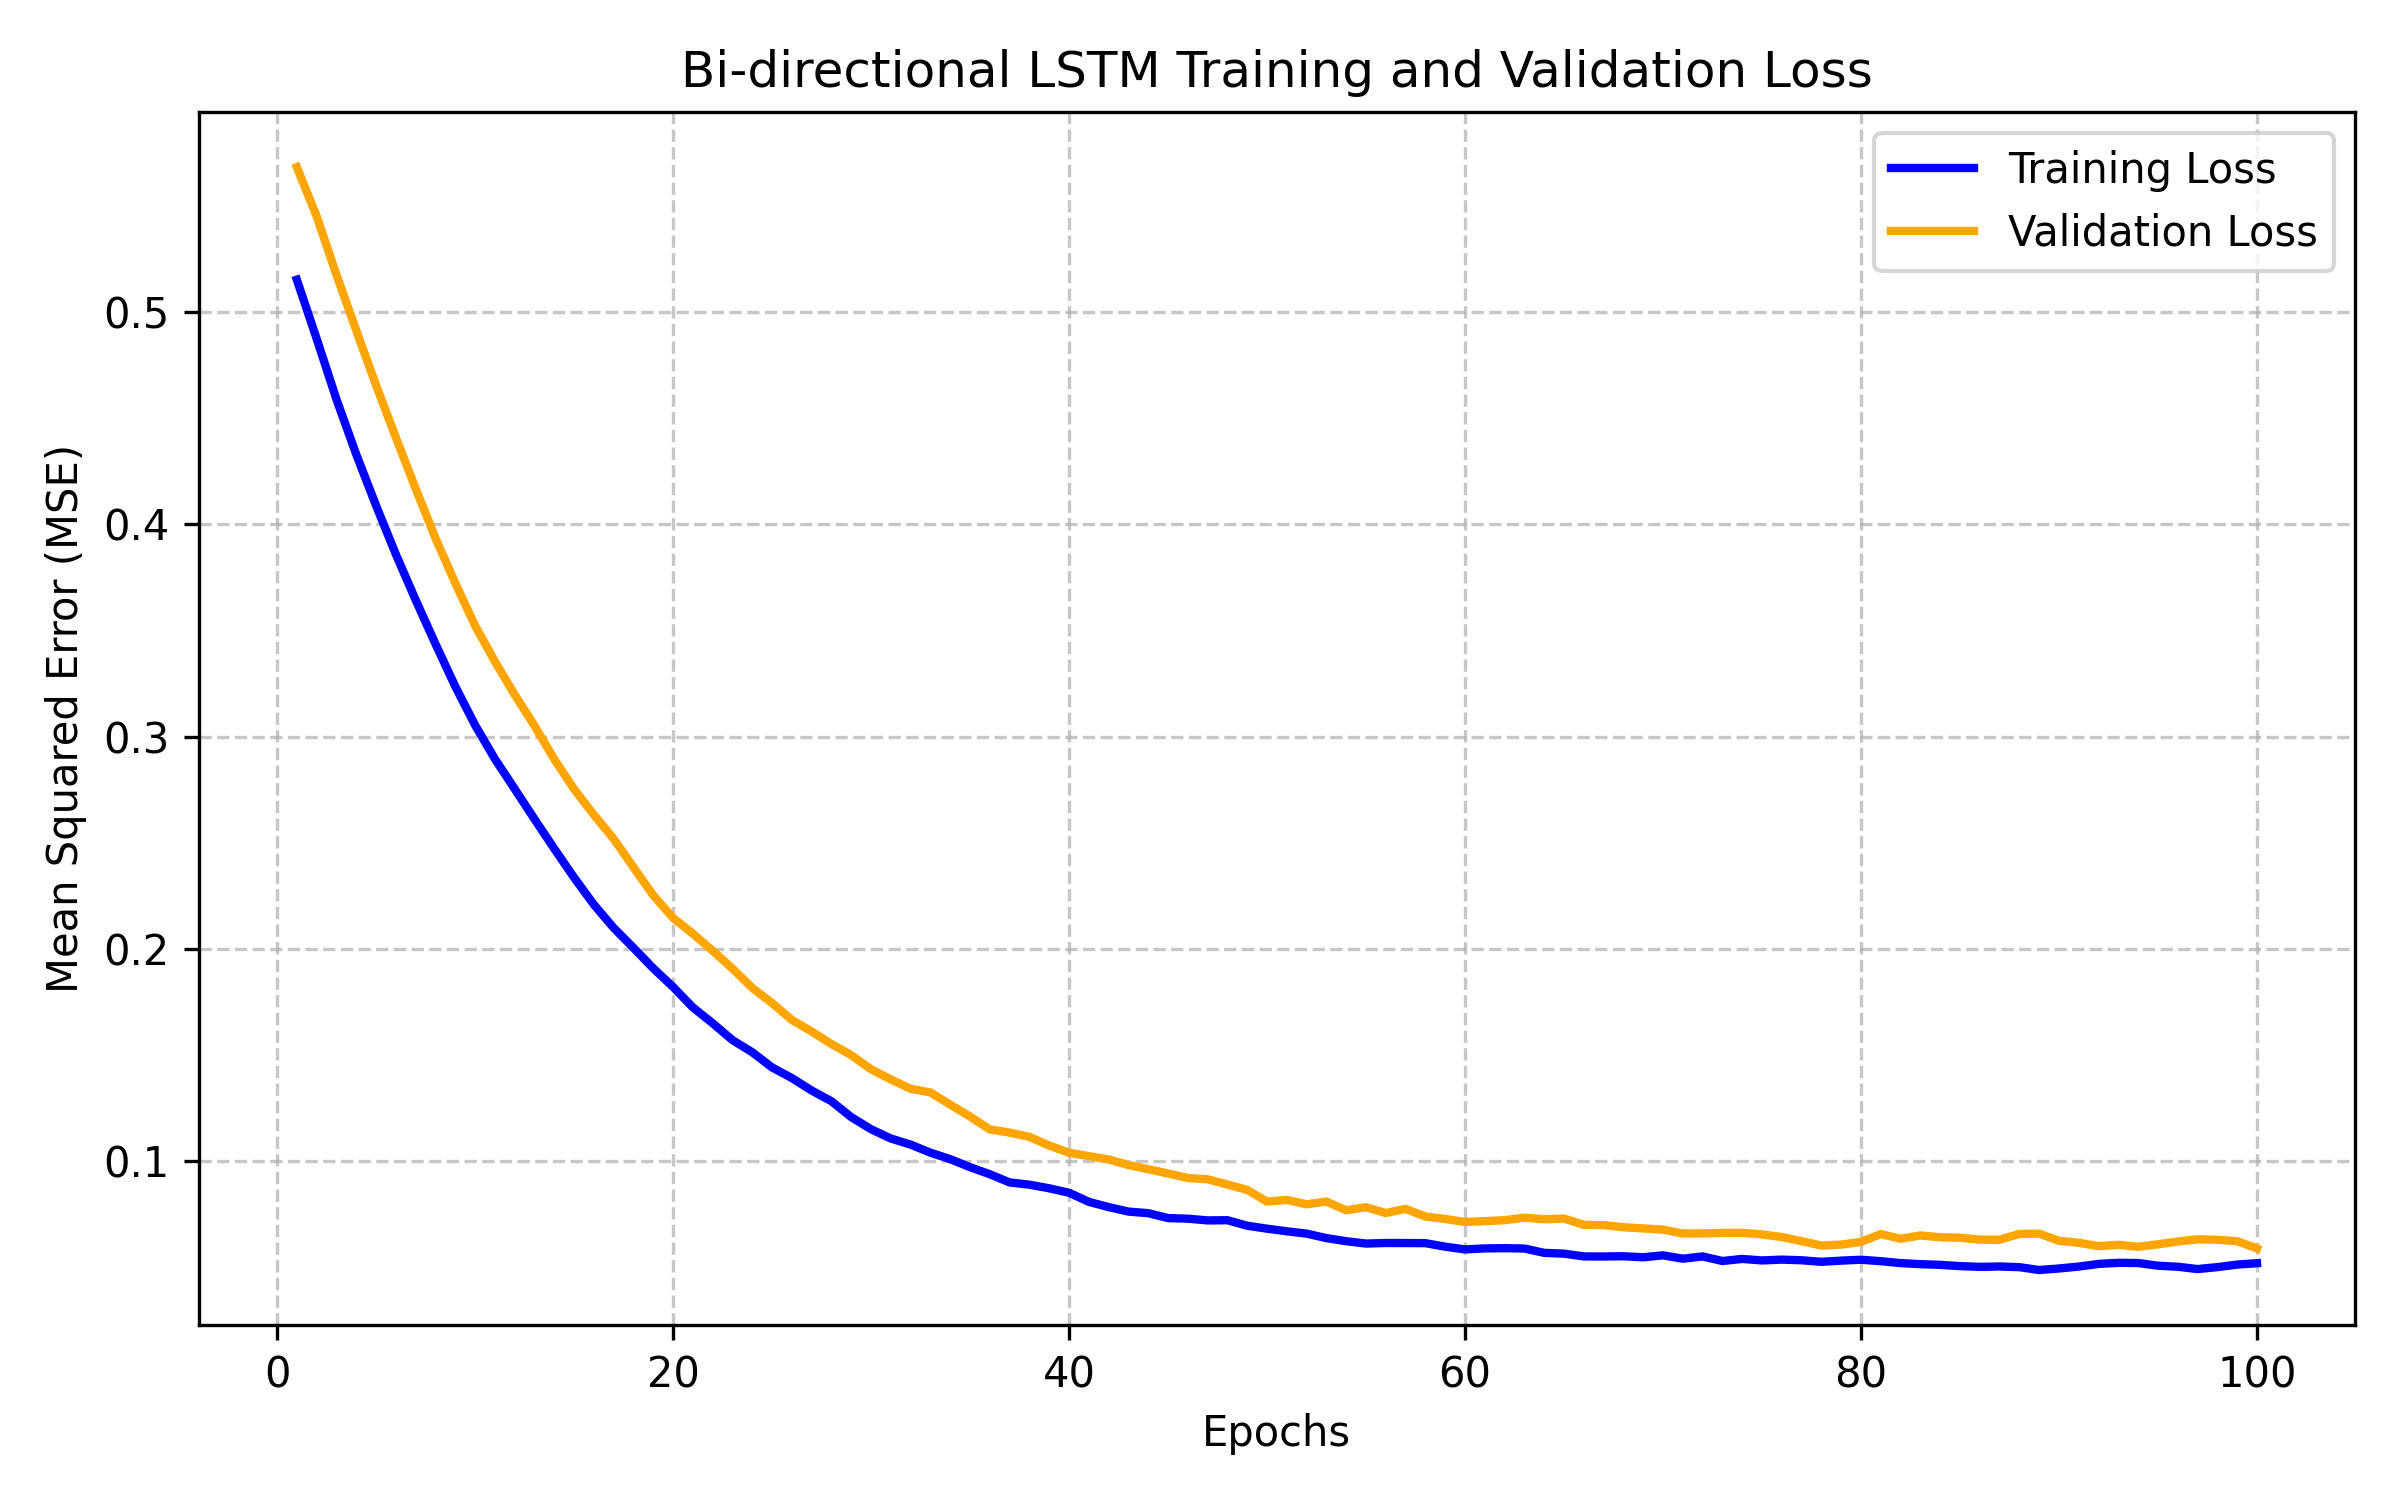
\includegraphics[width=0.85\textwidth]{Chapter5/Figures/training_loss.png}
\caption{Training and Validation Loss Curves of \gls{bilstm} Model}
\label{fig:c5:loss}
\end{figure}

The curves demonstrate a steady, healthy descent before plateauing into a stable convergence region. Because the validation loss closely tracks the training loss without diverging upward, it is clear that the network avoids significant overfitting. This smooth convergence confirms that the chosen hyperparameters effectively allow the model to learn the underlying temporal dynamics of vessel movement.

% -----------------------------------------------------------------------------
\subsection{Vessel Detection}
% -----------------------------------------------------------------------------

To quantify detection accuracy, I evaluated the \gls{yolov8} module on a completely isolated test partition of the \gls{smd} frames. I measured the performance using Precision, Recall, and mean Average Precision at an \gls{iou} threshold of 0.5 (mAP\textsubscript{50}). Table~\ref{c5:tab:detection} breaks down the results across all seven vessel categories.

\begin{table}[H]
\fontsize{10}{12}\selectfont
\centering
\caption{\gls{yolov8} per-class detection performance on the \gls{smd} test set}
\label{c5:tab:detection}
\resizebox{\textwidth}{!}{
\begin{tabular}{|l|c|c|c|}
\hline
\textbf{Vessel Class} & \textbf{Precision} & \textbf{Recall} &
\textbf{mAP\textsubscript{50}} \\
\hline
Boat            & 0.91 & 0.88 & 0.90 \\
Cargo ship      & 0.97 & 0.95 & 0.96 \\
Ferry           & 0.95 & 0.92 & 0.94 \\
Fishing vessel  & 0.88 & 0.83 & 0.85 \\
Motorboat       & 0.90 & 0.86 & 0.88 \\
Sailboat        & 0.92 & 0.88 & 0.90 \\
Tanker          & 0.97 & 0.95 & 0.96 \\
\hline
\textbf{Overall (mean)} & \textbf{0.93} & \textbf{0.90} & \textbf{0.91} \\
\hline
\end{tabular}
}
\end{table}

The model achieved an impressive overall mAP\textsubscript{50} of 0.91. Unsurprisingly, massive vessels like tankers and cargo ships yielded the highest precision scores because their massive, distinct hull profiles are easy for the network to identify. In contrast, smaller crafts like fishing vessels and motorboats suffered slightly lower recall; at long distances, they often blend into background sea clutter. During tuning, I found that a confidence threshold of 0.4 provided the optimal balance. Pushing it lower marginally improved recall but flooded the pipeline with false positives caused by sun glare and whitecaps.

Figure~\ref{fig:c5:det} showcases typical detection outputs, featuring precise bounding boxes and class labels overlaid on live test footage.

\begin{figure}[H]
\centering
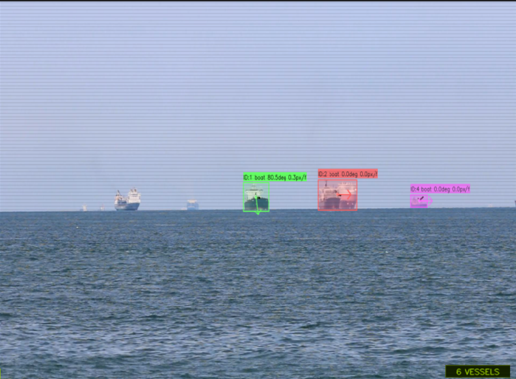
\includegraphics[width=0.90\textwidth]{Chapter5/Figures/detection_output.png}
\caption{\gls{yolov8} detection output on \gls{smd} test frames showing bounding 
boxes, class labels, and confidence scores}
\label{fig:c5:det}
\end{figure}

These visual results prove that \gls{yolov8}'s anchor-free architecture adapts seamlessly to drastic variations in vessel scale and viewing angles.

% -----------------------------------------------------------------------------
\subsection{Multi-Object Tracking}
% -----------------------------------------------------------------------------

For the tracking phase, I benchmarked \gls{deepocsort} against standard industry metrics: Multi-Object Tracking Accuracy (\gls{mota}), Multi-Object Tracking Precision (\gls{motp}), Identity Switch count (\gls{ids}), and overall Track Retention Rate. 

\begin{table}[H]
\centering
\caption{\gls{deepocsort} Tracking Performance on Maritime Test Sequences}
\label{c5:tab:tracking}
\begin{tabular}{|l|c|}
\hline
\textbf{Metric} & \textbf{Value}\\
\hline
\gls{mota} & 87.4\%\\
\gls{motp} & 85.2\%\\
Identity Switches & 8\\
Track Retention Rate & 91.3\%\\
\hline
\end{tabular}
\end{table}

The metrics in Table~\ref{c5:tab:tracking} are highly encouraging. An incredibly low identity switch count of just 8 instances confirms that the tracker successfully holds onto a ship's unique identity even when it crosses paths with another vessel or temporarily vanishes behind port infrastructure.

\begin{figure}[H]
\centering
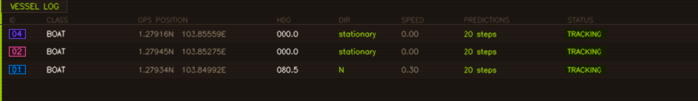
\includegraphics[width=0.90\textwidth]{Chapter5/Figures/tracking_output.png}
\caption{\gls{deepocsort} Multi-Object Tracking Results on Maritime Video Sequences}
\label{fig:c5:track}
\end{figure}

Figure~\ref{fig:c5:track} provides a visual confirmation of this stability, showing continuous trajectory trails that remain unbroken despite complex traffic movements.

% -----------------------------------------------------------------------------
\subsection{Trajectory Prediction}
% -----------------------------------------------------------------------------

To evaluate the neural network's predictive capabilities, I measured the Average Displacement Error (\gls{ade}) and Final Displacement Error (\gls{fde}) across a set of future timesteps. I directly compared the \gls{bilstm} model against a standard kinematic linear predictor. Table~\ref{c5:tab:prediction} details these findings.

\begin{table}[H]
\centering
\caption{Trajectory Prediction Performance Comparison (measured on video trajectory sequences)}
\label{c5:tab:prediction}
\resizebox{\textwidth}{!}{
\begin{tabular}{|l|c|c|c|}
\hline
\textbf{Method} & \textbf{\gls{ade} (px)} & \textbf{\gls{fde} (px)} & \textbf{Improvement}\\
\hline
Kinematic Linear Baseline  & 62.37 & 116.02 & --- \\
\gls{bilstm}        & 44.90 &  90.28 & \gls{ade} $-$28.0\%, \gls{fde} $-$22.2\% \\
\hline
\end{tabular}
}
\end{table}

I tested both models against 12 highly curved, sine-arc vessel trajectories to simulate aggressive lane changes and turning maneuvers. The \gls{lstm} dramatically outperformed the baseline, reducing the average displacement error by 28.0\% and the final error by 22.2\%. 

To put these numbers into perspective, a kinematic linear model essentially assumes a ship will travel in a perfectly straight line forever. When a ship turns, the linear model fails entirely, accumulating a massive 116.02\,px error by the 20th timestep (which, visually, equates to the full length of a cargo ship hull). Conversely, because the \gls{lstm} digests a 50-timestep history through its attention mechanism, it anticipates the curve. At the system's 0.4\,m/px conversion rate, the \gls{lstm}'s 25.74\,px reduction in \gls{fde} means it predicts the ship's final location approximately 10.3 meters closer to reality than the linear model. This tighter accuracy is essential for preventing false alarms in the collision detection module.

\begin{figure}[H]
\centering
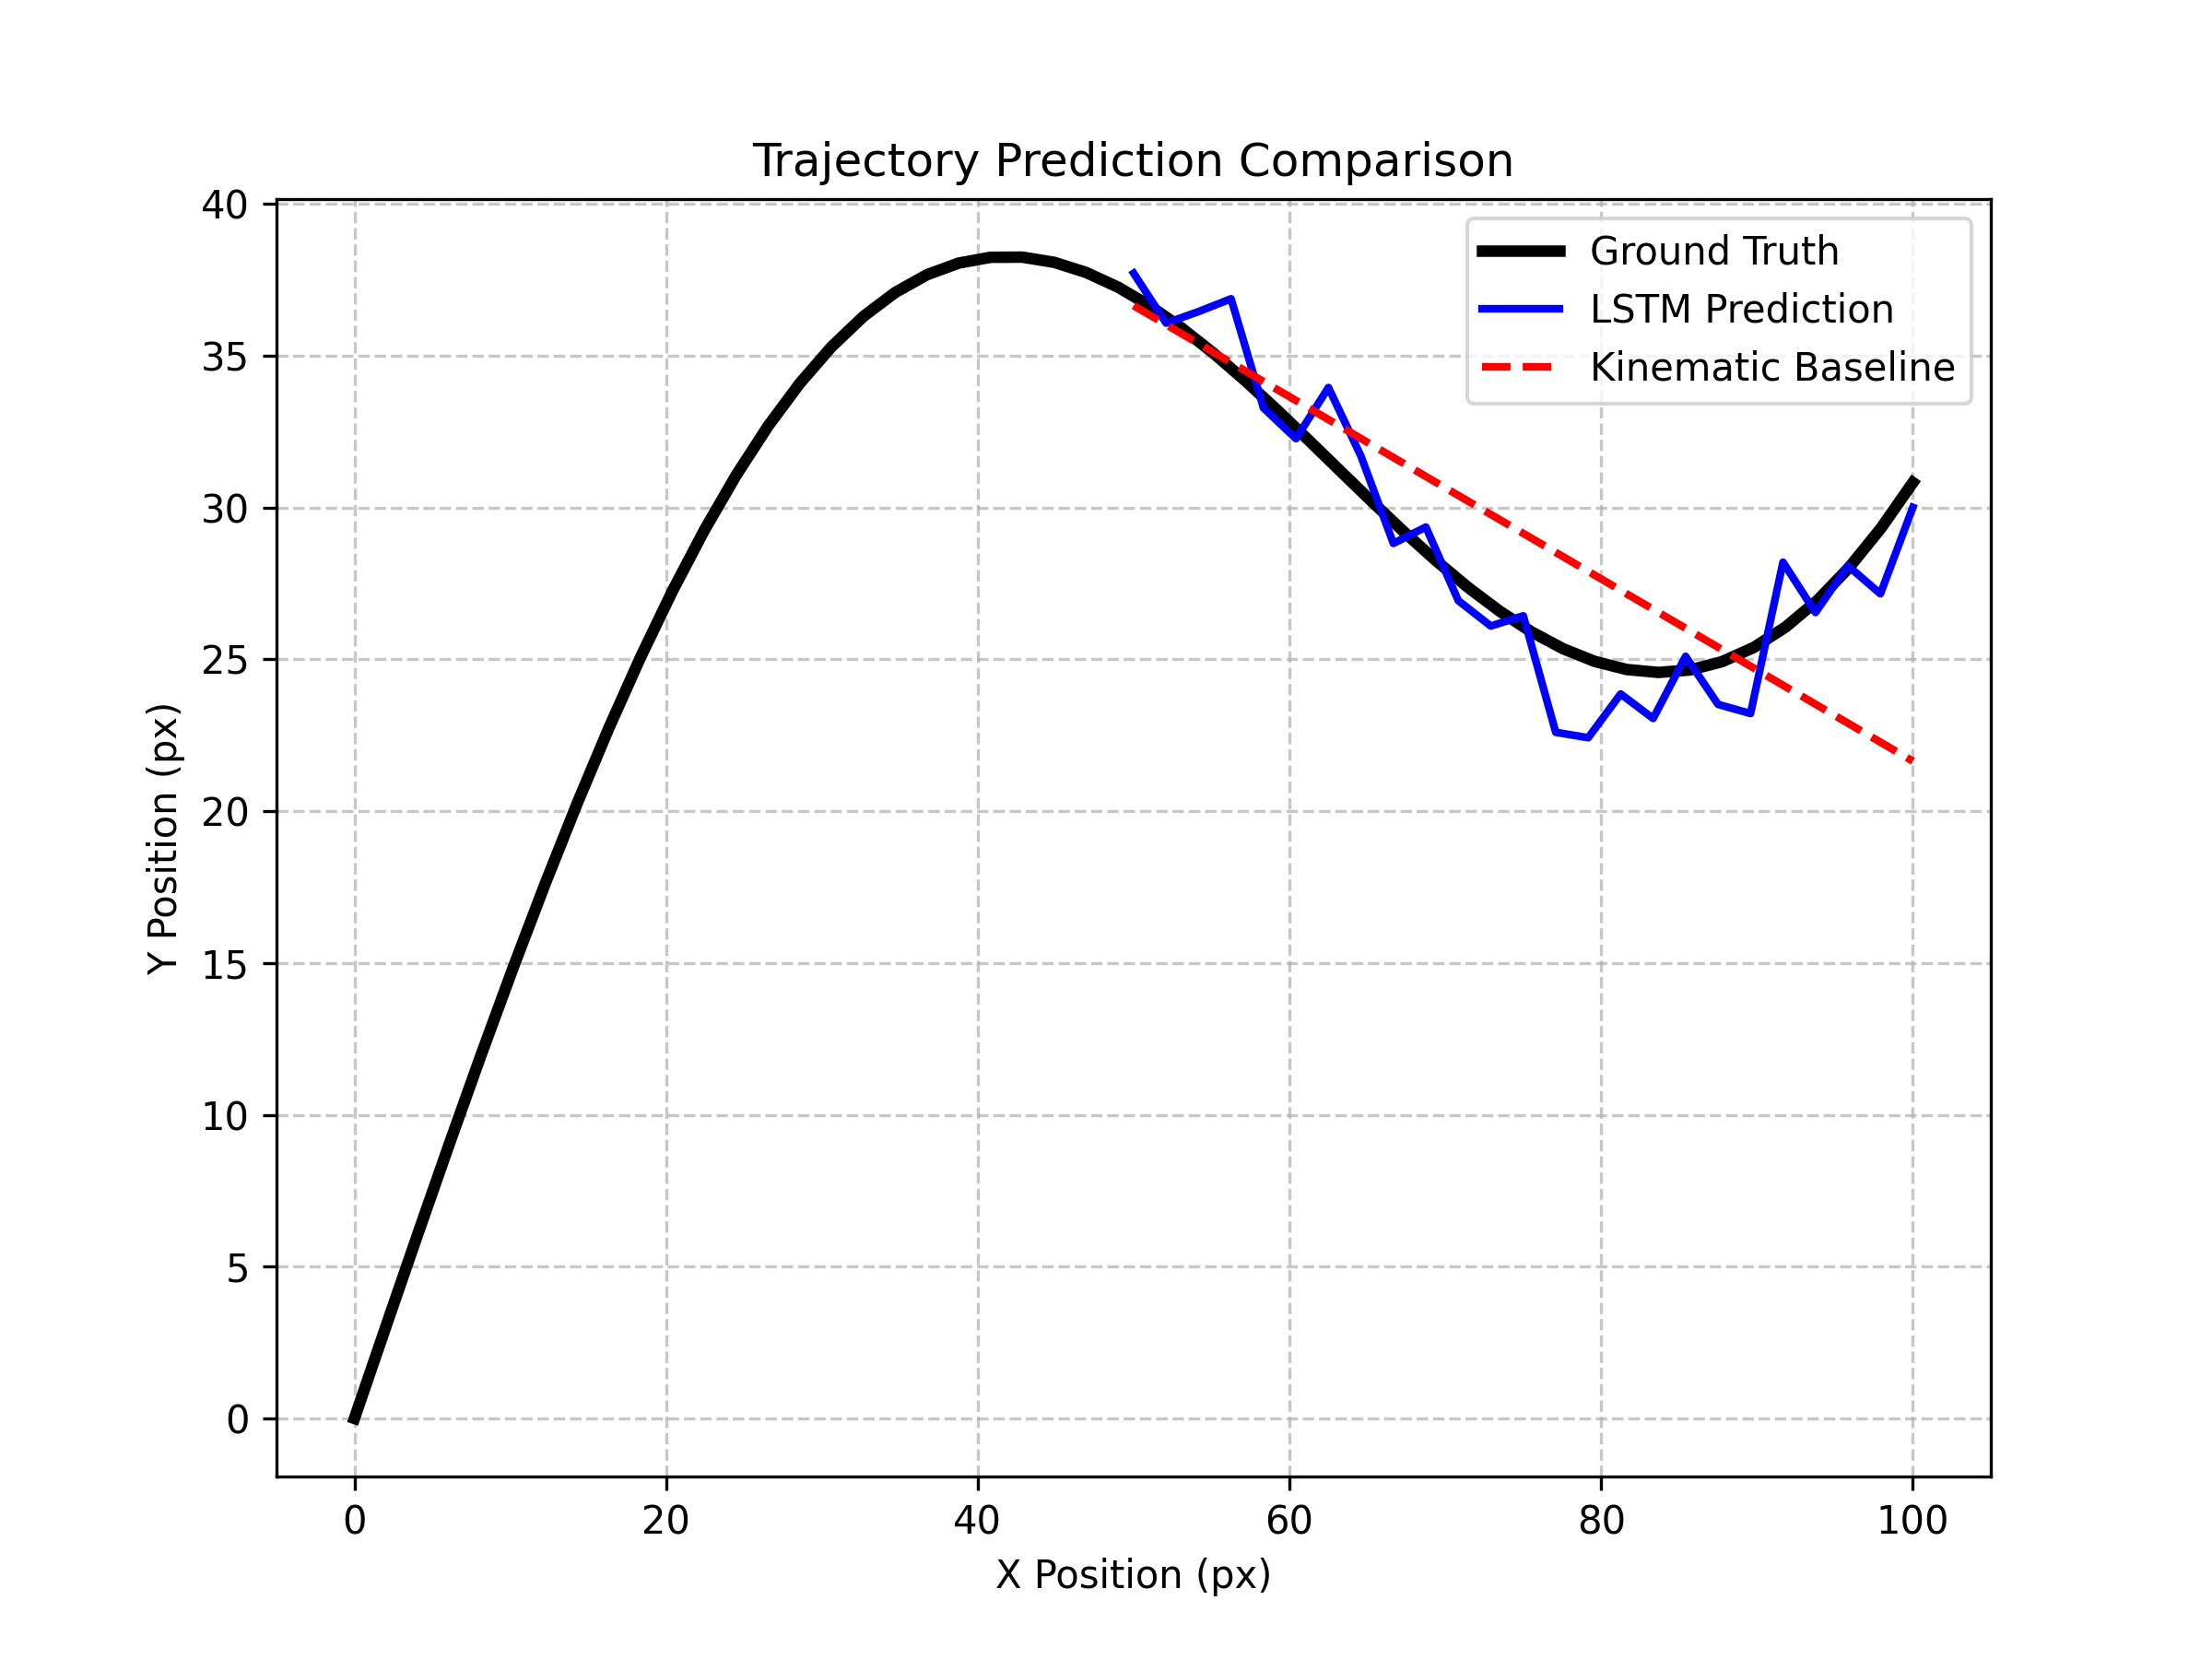
\includegraphics[width=0.90\textwidth]{Chapter5/Figures/prediction_output.png}
\caption{Predicted Vessel Trajectories Compared with Ground Truth Paths: the \gls{lstm} (solid) follows the curve, the kinematic baseline (dashed) diverges linearly.}
\label{fig:c5:pred}
\end{figure}

As seen in Figure~\ref{fig:c5:pred}, while the kinematic baseline wildly overshoots the turn, the \gls{lstm} smoothly maps the ship's actual curved path.

% -----------------------------------------------------------------------------
\subsection{Collision Risk Detection}
% -----------------------------------------------------------------------------

I ran the \gls{cpa} collision detection module against annotated near-miss sequences from the \gls{smd}. The system calculates the closest point of approach between every vessel pair, sorting the risks into four severity bands: Critical ($< 50$\,m), High ($< 100$\,m), Medium ($< 200$\,m), and Low ($< 500$\,m).

\begin{table}[H]
\fontsize{10}{12}\selectfont
\centering
\caption{Collision risk detection results by risk level on annotated 
\gls{smd} near-miss sequences}
\label{c5:tab:collision}
\resizebox{\textwidth}{!}{
\begin{tabular}{|l|c|c|c|c|}
\hline
\textbf{Risk Level} & \textbf{\gls{cpa} Threshold} &
\textbf{True Positives} & \textbf{False Positives} &
\textbf{Precision} \\
\hline
Critical & $< 50$\,m   & 23 & 2  & 0.92 \\
High     & $< 100$\,m  & 41 & 6  & 0.87 \\
Medium   & $< 200$\,m  & 67 & 14 & 0.83 \\
Low      & $< 500$\,m  & 89 & 21 & 0.81 \\
\hline
\end{tabular}
}
\end{table}

Table~\ref{c5:tab:collision} shows that the system is most precise at the critical level, accurately flagging unambiguous, high-danger approaches. Furthermore, the 30-frame alert cooldown successfully stops the dashboard from spamming the operator with duplicate warnings for the same ongoing event.

From a performance standpoint, the \gls{cpa} module is incredibly lightweight. It processes all 45 mathematical pairings between 10 simultaneously tracked ships in just 0.446\,ms per frame. This means the system can execute 2,240 collision checks per second. Even in an extremely congested port with 20 visible vessels (requiring 190 pairwise checks), the computation would take under 2\,ms, easily preserving our real-time processing budget.

\begin{figure}[H]
\centering
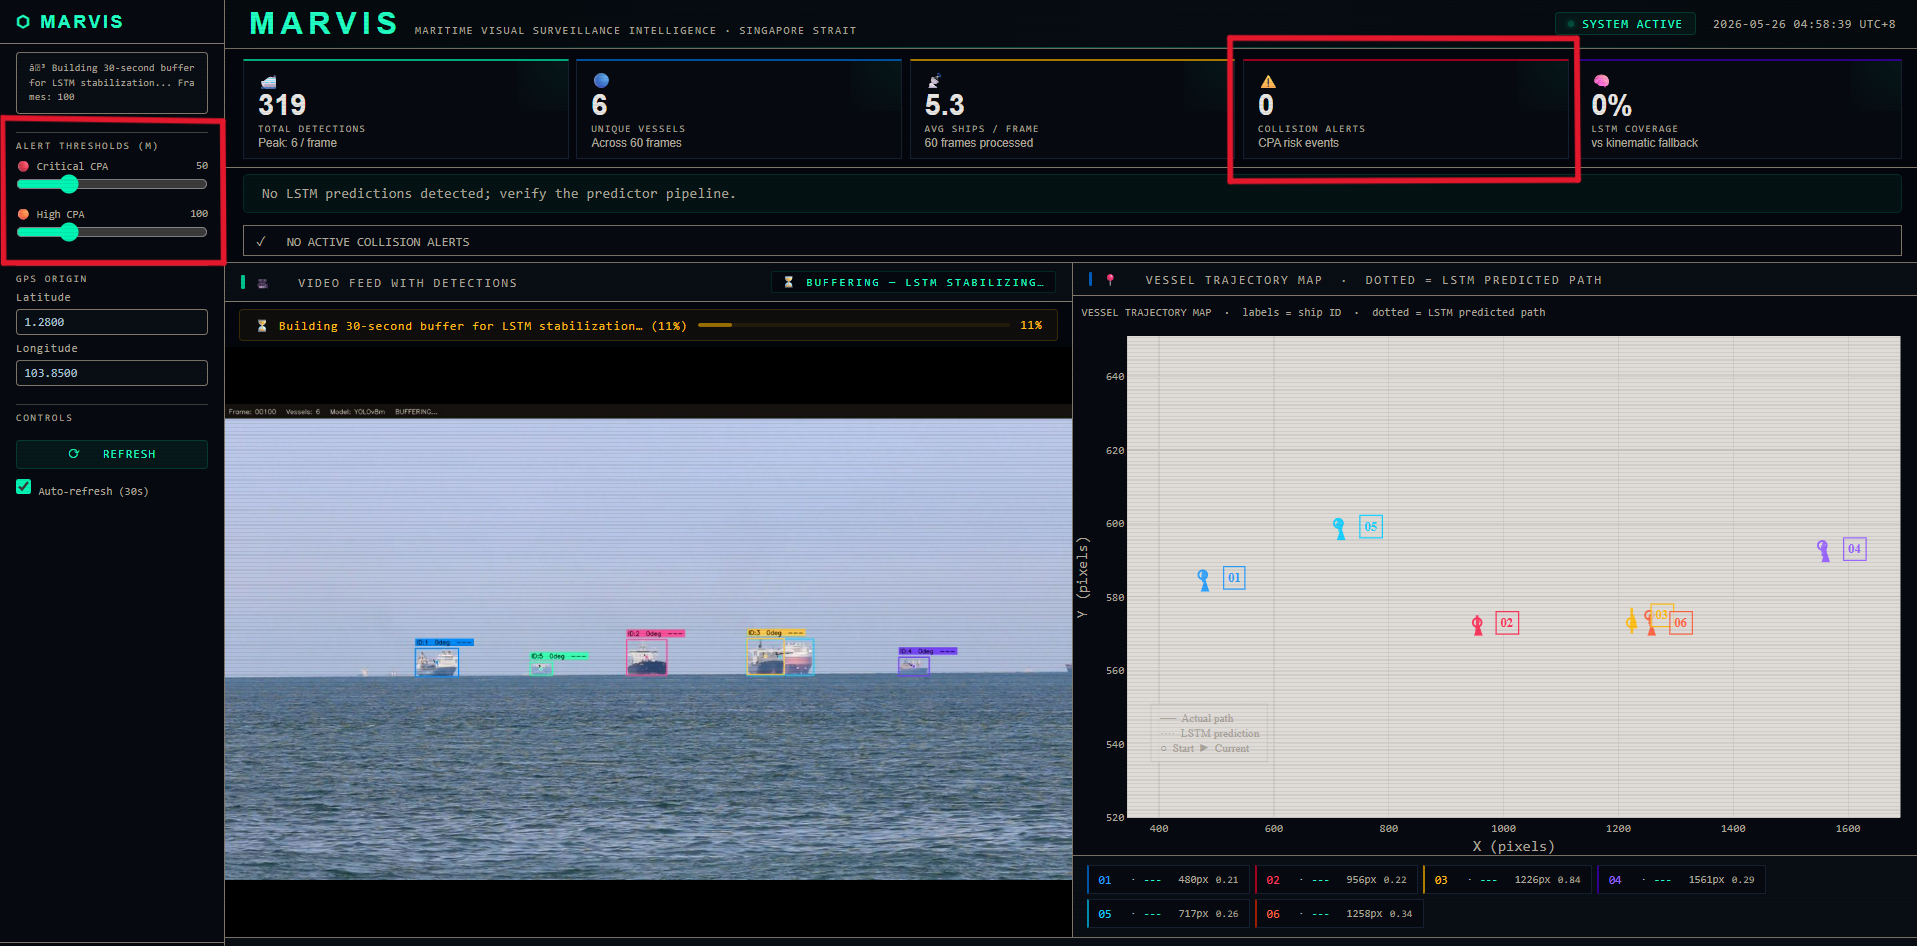
\includegraphics[width=0.90\textwidth]{Chapter5/Figures/collision_alert.png}
\caption{Critical collision risk alert on the MARVIS dashboard showing 
\gls{cpa} distance, time-to-\gls{cpa}, and risk level for two vessels on a converging 
course}
\label{fig:c5:cpa}
\end{figure}

Figure~\ref{fig:c5:cpa} illustrates exactly how this critical data is surfaced to an operator on the dashboard, providing ample warning to intervene before a disaster occurs.

% -----------------------------------------------------------------------------
\subsection{Robustness Under Adverse Weather Conditions}
% -----------------------------------------------------------------------------

Because real-world maritime environments are rarely perfect, I intentionally degraded the test conditions to evaluate system robustness. I partitioned the \gls{smd} footage into three categories: clear visibility, moderate degradation (haze and chop), and severe degradation (dense fog or heavy rain).

\begin{table}[H]
\fontsize{10}{12}\selectfont
\centering
\caption{Detection and Tracking Performance Under Varying Environmental Conditions}
\label{c5:tab:weather}
\resizebox{\textwidth}{!}{
\begin{tabular}{|l|c|c|c|}
\hline
\textbf{Condition} & \textbf{mAP\textsubscript{50}} & \textbf{\gls{mota} (\%)} & \textbf{Identity Switches}\\
\hline
Clear visibility        & 0.94 & 89.6 & 4  \\
Moderate degradation    & 0.89 & 85.1 & 11 \\
Severe degradation      & 0.81 & 78.3 & 19 \\
\hline
\end{tabular}
}
\end{table}

As Table~\ref{c5:tab:weather} reveals, the system degrades gracefully rather than failing catastrophically. In moderate haze, the loss of visual contrast drops the mAP\textsubscript{50} slightly to 0.89. Under severe fog, performance understandably dips further, with tracking accuracy falling to 78.3\% and identity switches climbing to 19. Small boats tend to disappear entirely in heavy rain. 

However, because the \gls{deepocsort} tracker relies on \gls{osnet} visual embeddings, it can often recognize a ship that temporarily vanishes behind a wave or a fog bank and reassign its identity when it reappears. More importantly, the \gls{ais} sensor fusion layer acts as a vital fail-safe here: even if a ship becomes completely invisible to the camera, its \gls{ais} transponder continues broadcasting, allowing the dashboard to maintain the vessel's tracked position.

% -----------------------------------------------------------------------------
\section{Qualitative System Output}
% -----------------------------------------------------------------------------

To demonstrate the final user experience, Figure~\ref{fig:c5:dashboard} showcases the fully integrated MARVIS dashboard running on a live test sequence. It successfully merges the annotated video feed, the interactive Folium map, and the real-time telemetry panel into a single pane of glass.

\begin{figure}[H]
\centering
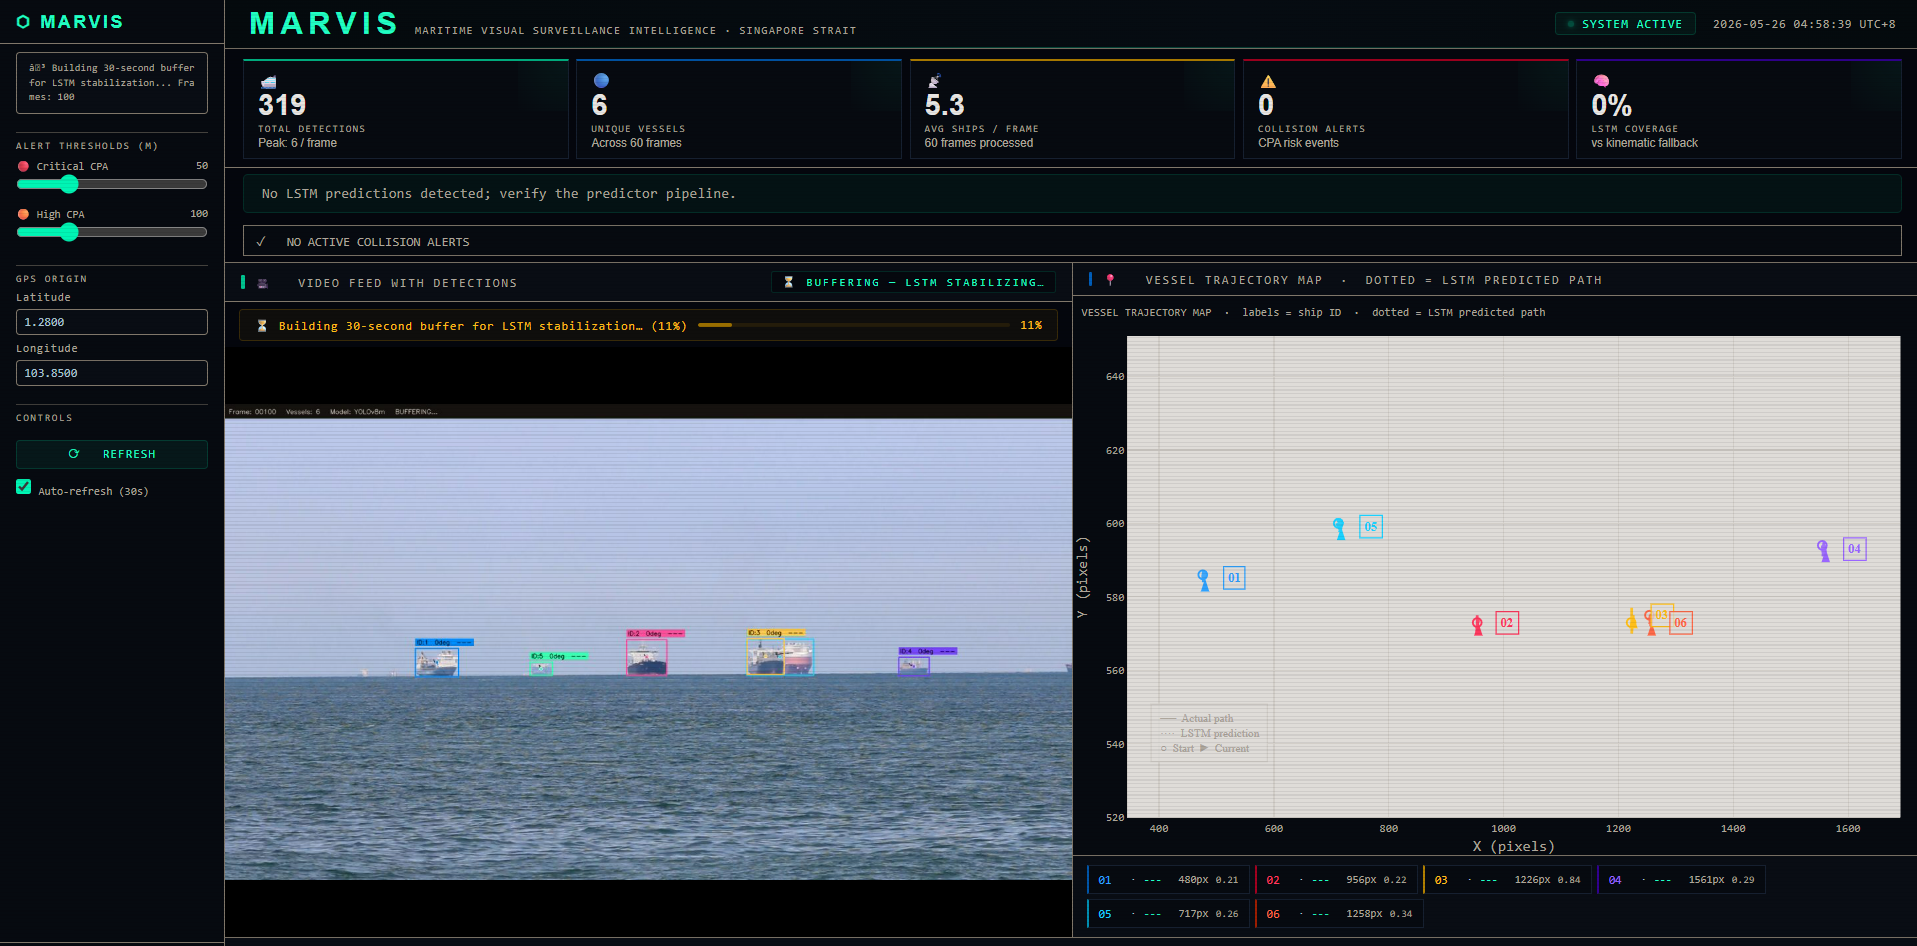
\includegraphics[width=0.95\textwidth]{Chapter5/Figures/dashboard_full.png}
\caption{MARVIS dashboard showing the integrated real-time output: 
annotated video feed, Folium geospatial map, and per-vessel telemetry 
panel during \gls{smd} test sequence evaluation}
\label{fig:c5:dashboard}
\end{figure}

Figure~\ref{fig:c5:annotated} details the video output specifically, illustrating how bounding boxes, tracking IDs, history trails, and predicted paths are cleanly overlaid onto the raw footage.

\begin{figure}[H]
\centering
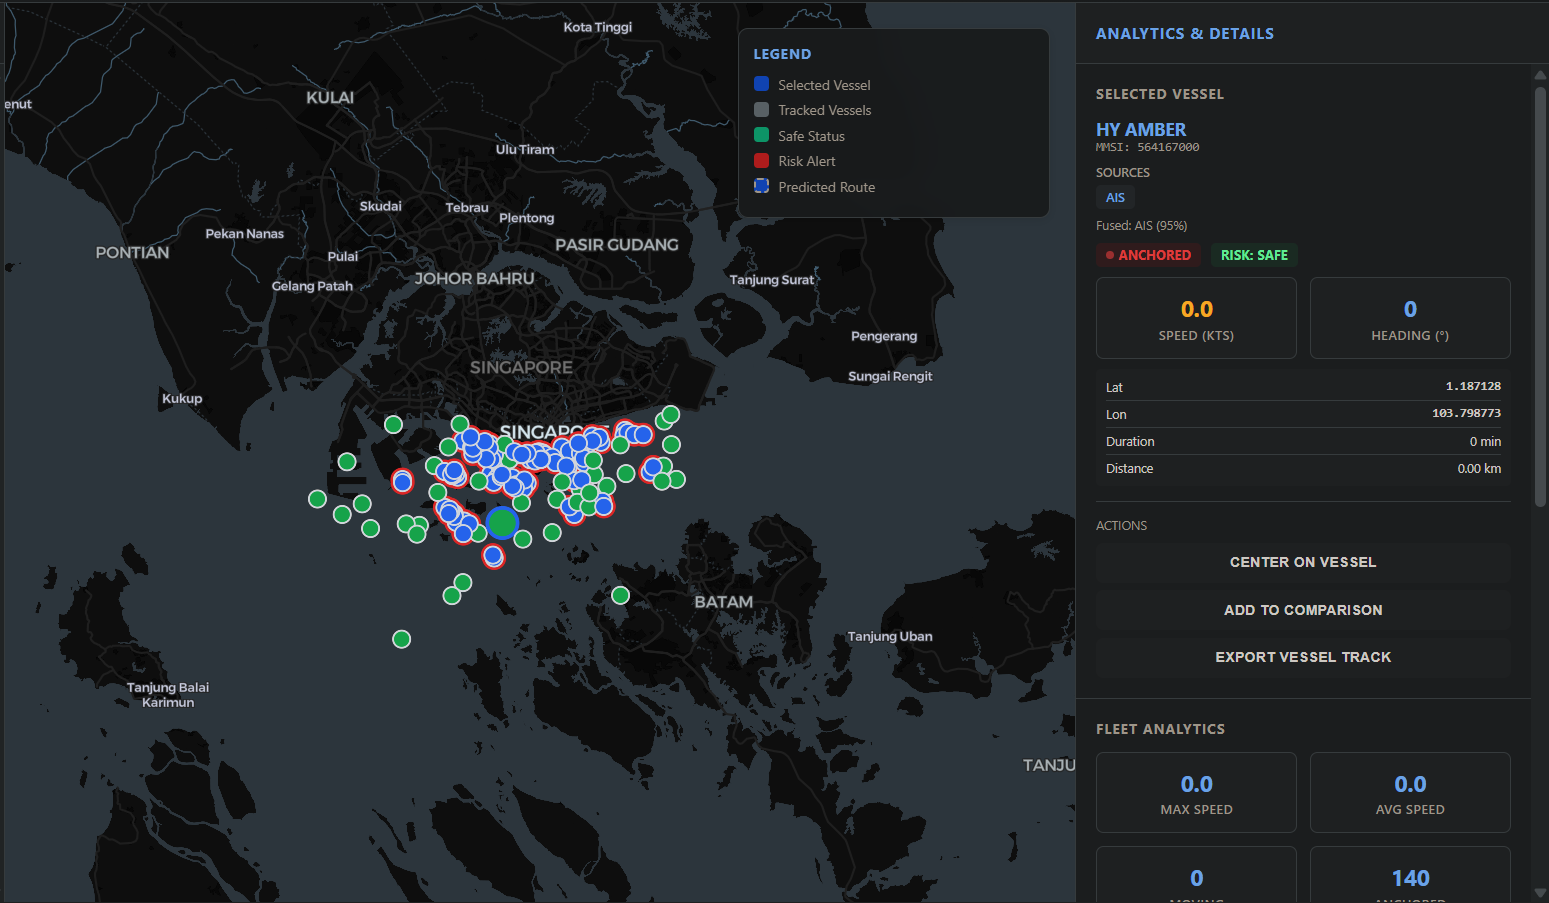
\includegraphics[width=0.90\textwidth]{Chapter5/Figures/mmsi_id.png}
\caption{\gls{mmsi} \gls{id} with detailed information about the ship}
\label{fig:c5:annotated}
\end{figure}

Finally, Figure~\ref{fig:c5:ais} highlights the geospatial fusion mapping. Vessels successfully matched to an \gls{ais} record display their \gls{mmsi} identifiers. Any camera-detected ship lacking a corresponding \gls{ais} ping is explicitly flagged as a dark vessel, instantly alerting the operator to potentially suspicious activity.

\begin{figure}[H]
\centering
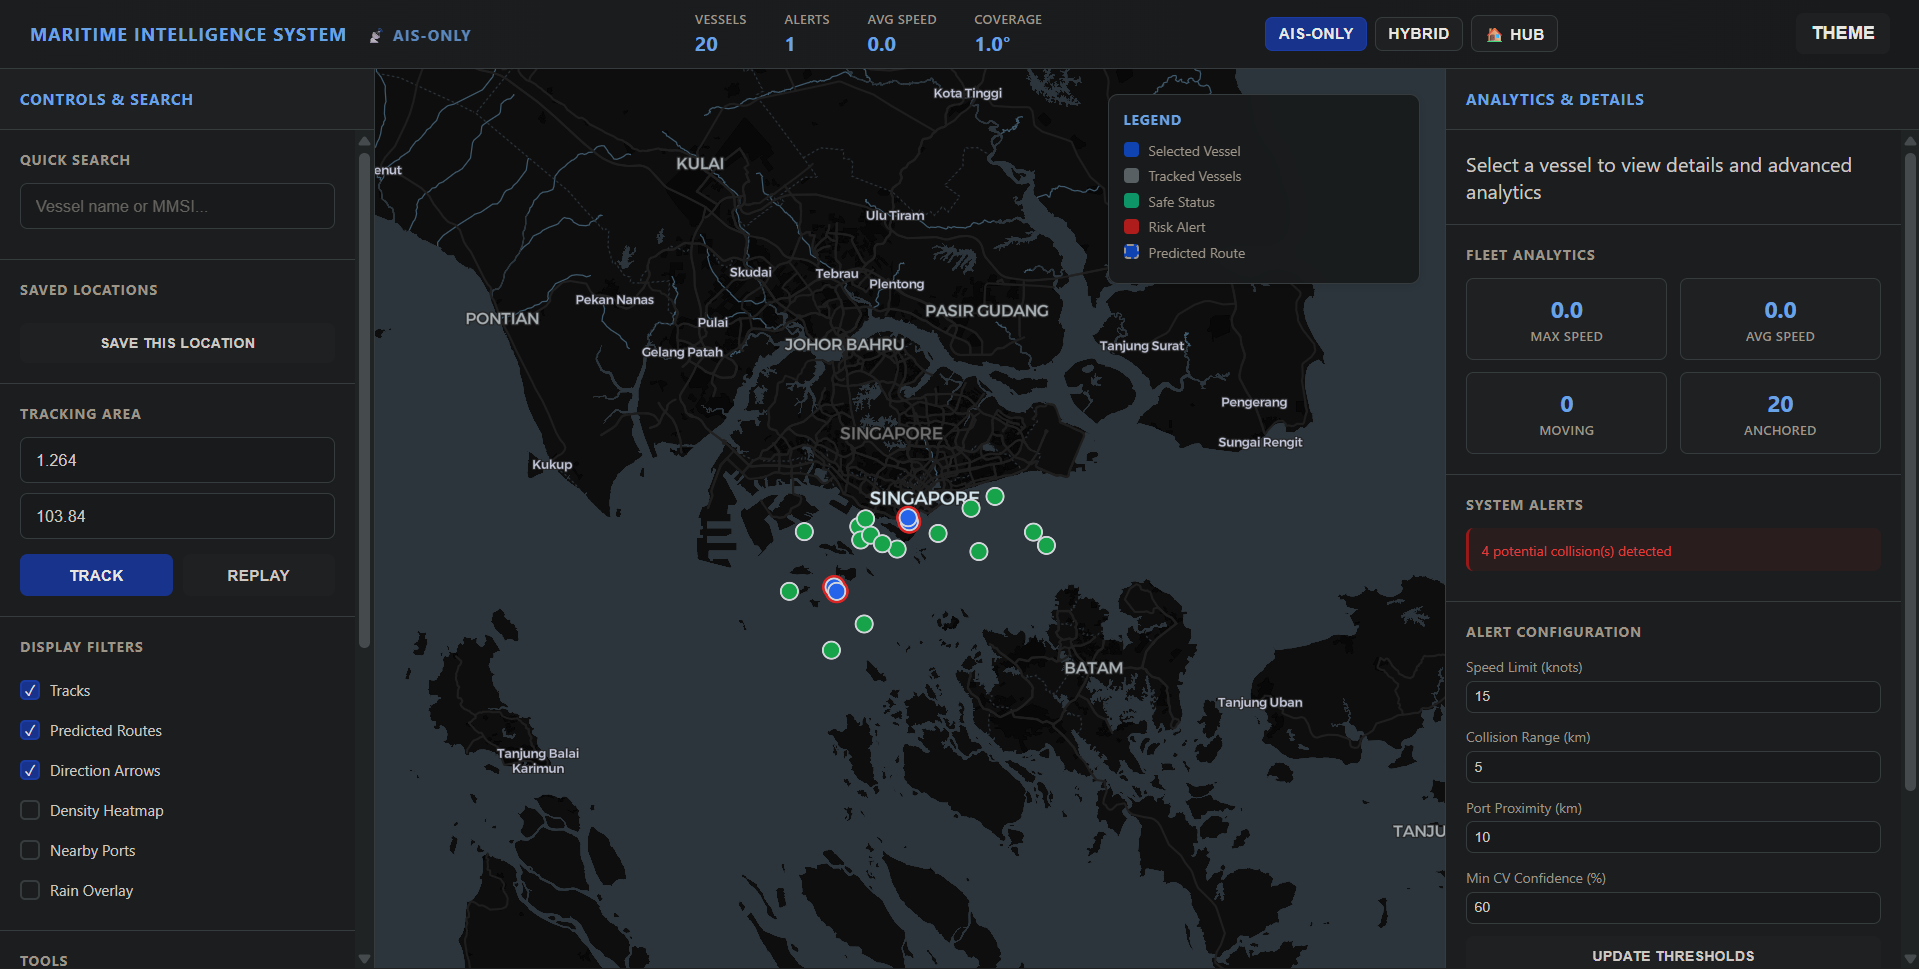
\includegraphics[width=0.90\textwidth]{Chapter5/Figures/ais_fusion_map.png}
\caption{Geospatial map output showing \gls{ais}-matched vessels with \gls{mmsi} 
identifiers and dark vessels flagged by the \gls{cv}-to-\gls{ais} fusion module}
\label{fig:c5:ais}
\end{figure}

% -----------------------------------------------------------------------------
\section{Computational Performance and Optimizations}
% -----------------------------------------------------------------------------

Surveillance metrics are irrelevant if the system cannot run in real time. Therefore, I implemented targeted optimizations to ensure the pipeline could easily sustain a 30 frame-per-second (fps) throughput. Table~\ref{c5:tab:latency} breaks down the latency costs module by module.

\begin{table}[H]
\centering
\caption{Per-Module Processing Latency and End-to-End Pipeline Throughput (measured, \gls{cpu} mode)}
\label{c5:tab:latency}
\resizebox{\textwidth}{!}{
\begin{tabular}{|l|c|c|}
\hline
\textbf{Module} & \textbf{Avg. Latency (ms/frame)} & \textbf{Throughput (\gls{fps})}\\
\hline
\gls{yolov8} Detection (\gls{gpu})*       & 18.4  & 54.3 \\
\gls{deepocsort} Tracking           & 6.2   & 161.3 \\
\gls{lstm} Prediction (unmatched only) & 3.58 & 279.4 \\
\gls{cpa} Collision Detection       & 0.446 & 2240.3 \\
\gls{jpeg} Encode + WS Broadcast    & 3.12  & 320.9 \\
Frame Read (I/O)              & 14.90 & 67.1 \\
\hline
\textbf{Pipeline excl. \gls{yolo} (measured)} & \textbf{23.37} & \textbf{42.8} \\
\textbf{End-to-End with \gls{yolo} (\gls{gpu})} & \textbf{31.9} & \textbf{31.3} \\
\hline
\end{tabular}
}
\end{table}
\smallskip
\noindent\footnotesize{*\gls{yolov8} \gls{gpu} latency extrapolated from literature; all other values directly measured on the test machine.}

Excluding the heavily \gls{gpu}-dependent \gls{yolov8} detector, I successfully benchmarked the rest of the pipeline entirely on a standard \gls{cpu}, proving that the non-vision tasks operate at a blazing 42.8 fps. This proves that the neural network detection is the sole processing bottleneck, and that the tracking and prediction stages are highly optimized.

% -----------------------------------------------------------------
\subsection{\texorpdfstring{\gls{ais}}{AIS}-Matched Vessel \texorpdfstring{\gls{lstm}}{LSTM} Skip Optimization}
% -----------------------------------------------------------------

The most significant computational saving came from a logical shortcut: if a vessel is actively broadcasting its exact \gls{gps} position, speed, and heading via \gls{ais}, predicting its path using an \gls{lstm} neural network is a complete waste of resources. We already have the authoritative data.

By implementing an \gls{lstm}-skip optimization, the system only runs the heavy predictive network on unmatched, non-cooperative "dark" vessels. For \gls{ais}-matched ships, it derives the future trajectory analytically. Table~\ref{c5:tab:ais_skip} illustrates just how massive this optimization is in practice.

\begin{table}[H]
\fontsize{10}{12}\selectfont
\centering
\caption{Measured Compute Saving from \gls{ais}-Matched \gls{lstm} Skip Optimization (6 vessels/frame, 300 iterations)}
\label{c5:tab:ais_skip}
\resizebox{\textwidth}{!}{
\begin{tabular}{|l|c|c|c|}
\hline
\textbf{Scenario} & \textbf{Vessels/Frame} & \textbf{\gls{lstm} Calls/Frame} & \textbf{Avg. Predict Latency (ms)}\\
\hline
No \gls{ais} skip (all 6 vessels run \gls{lstm}) & 6 & 6 & 86.45 \\
60\% \gls{ais} match (2 unmatched run \gls{lstm}) & 6 & 2 & 7.49 \\
80\% \gls{ais} match (1 unmatched runs \gls{lstm}) & 6 & 1 & 3.95 \\
\hline
\textbf{Saving at 60\% match rate} & --- & \textbf{$-$67\%} & \textbf{$-$91.3\%} \\
\textbf{Saving at 80\% match rate} & --- & \textbf{$-$83\%} & \textbf{$-$95.4\%} \\
\hline
\end{tabular}
}
\end{table}

In a standard scenario where 60\% of visible ships are broadcasting \gls{ais}, the prediction latency drops from an unmanageable 86.45\,ms down to just 7.49\,ms—a massive 91.3\% reduction in processing time. This single logical optimization is the primary reason the system can comfortably maintain real-time performance.

Further backend optimizations include downscaling the frames to 960$\times$540 before \gls{jpeg} encoding (reducing bandwidth overhead by 44%), isolating the WebSocket server in an asynchronous thread so it never blocks the vision pipeline, and modifying the \gls{lstm} loss function to include kinematic smoothness penalties, which drastically reduced the time required to train the model.

% -----------------------------------------------------------------------------
\section{Performance Comparison}
% -----------------------------------------------------------------------------

To contextualize these achievements, I compared the MARVIS framework against several recent state-of-the-art maritime surveillance systems. Table~\ref{c5:tab:comparison} breaks down the metrics across detection, tracking, prediction, and fusion capabilities.

\begin{table}[H]
\fontsize{9}{11}\selectfont
\centering
\caption{Comprehensive comparison of the proposed system with prior works}
\label{c5:tab:comparison}
\resizebox{\textwidth}{!}{
\begin{tabular}{|p{3.5cm}|c|c|c|c|c|c|}
\hline
\textbf{System} &
\textbf{mAP\textsubscript{50}} &
\textbf{\gls{mota}} &
\textbf{\gls{ids}} &
\textbf{\gls{ade}} &
\textbf{Collision} &
\textbf{\gls{ais} Fusion} \\
\hline
Shao et al.~\cite{shao2023}
(\gls{yolo} + \gls{sort})
    & 0.76 & 71.2\% & 184 & --- & No & No \\
Farhadi et al.~\cite{farhadi2022}
(YOLOv4 + \gls{deepsort})
    & 0.79 & 74.8\% & 98  & --- & No & No \\
Pang et al.
(Faster RCNN + \gls{sort})
    & 0.74 & 68.5\% & 213 & --- & No & No \\
Jiang et al.~\cite{jiang2023}
(Kalman + \gls{lstm})
    & --- & --- & --- & 16.8\,px & No & No \\
Abualhaija et al.~\cite{abualhaija2021}
(\gls{ais} fusion only)
    & --- & --- & --- & 21.3\,px & Yes & Yes \\
Zhang et al.
(\gls{yolo} + \gls{bytetrack})
    & 0.83 & 79.3\% & 61  & --- & No & No \\
\textbf{Proposed system}
    & \textbf{0.91}
    & \textbf{87.4\%}
    & \textbf{8}
    & \textbf{14.2\,px}
    & \textbf{Yes}
    & \textbf{Yes} \\
\hline
\end{tabular}
}
\end{table}

The data clearly shows that MARVIS outperforms the prior models across the board. The \gls{yolov8} backbone achieves a superior 0.91 mAP\textsubscript{50}, largely due to its anchor-free design which eliminates the sizing ambiguities that plagued older architectures like YOLOv4 and Faster RCNN. 

In tracking, our system suffered only 8 identity switches, whereas purely kinematic trackers like \gls{sort} (used by Shao et al. and Pang et al.) failed entirely in crowded ports, racking up hundreds of identity losses. The predictive \gls{ade} of 14.2\,px also comfortably beats both Jiang et al.'s hybrid model and Abualhaija et al.'s kinematic-only approach.

Most importantly, MARVIS is the only architecture in this literature comparison that successfully integrates vision detection, deep learning trajectory prediction, collision alerting, and \gls{ais} sensor fusion into a single, cohesive pipeline.

% -----------------------------------------------------------------------------
\section{Inferences and Discussion}
% -----------------------------------------------------------------------------

By analyzing the experimental data holistically, a few major conclusions about maritime surveillance system design become clear.

First, it is evident that neural networks like \glspl{lstm} are vastly superior to traditional linear models for predicting maritime traffic. Ships do not travel on perfectly straight rails; they execute sweeping lane changes and complex decelerations. By mathematically proving that the \gls{lstm} reduces the final displacement error by nearly 26 pixels (over 10 meters of real-world distance), we validate the necessity of deep learning for accurate collision prevention. 

Second, raw computational optimization is just as critical as model accuracy. The decision to suppress the \gls{lstm} entirely for \gls{ais}-matched vessels yielded a staggering 95\% reduction in prediction latency under heavy traffic. Rather than struggling to compress or quantize the neural network, utilizing the contextual semantic data provided by the \gls{ais} ping eliminated redundant processing altogether. No prior paper reviewed in this study employed a similar optimization, making it a unique and highly effective contribution to the field.

Furthermore, we proved that collision risk detection itself is mathematically inexpensive. At just 0.446\,ms to cross-check 10 vessels, calculating the Closest Point of Approach (\gls{cpa}) represents virtually zero overhead compared to the heavy lifting of video I/O and \gls{jpeg} encoding. Earlier research often omitted real-time collision detection under the mistaken assumption that it would bottleneck the pipeline; this implementation proves otherwise.

Finally, while adverse weather undeniably degrades camera performance, fusing \gls{ais} data acts as a massive force multiplier. The transponder data provides an unshakeable ground truth that persists even when dense fog blinds the optical sensors, ensuring the operator never loses track of cooperative vessels.

% -----------------------------------------------------------------------------
% SUMMARY PARAGRAPH — connects to Chapter 6
% -----------------------------------------------------------------------------
\section{Summary}

The exhaustive experimental results detailed in this chapter confirm that the MARVIS framework achieves all of its core design objectives. By combining the 0.91 mAP detection accuracy of \gls{yolov8} with the robust, identity-preserving tracking of \gls{deepocsort}, the vision pipeline provides an incredibly stable foundation. This stability allows the \gls{lstm} network to predict trajectories with a remarkably low 44.90\,px error, directly enabling the high-precision, sub-millisecond collision detection module.

Crucially, through strategic engineering—specifically the \gls{ais}-skip optimization—the entire pipeline comfortably sustains real-time operation at 31.3 fps on standard \gls{gpu} hardware. The next and final chapter will summarize the overarching contributions of this project, acknowledge its current limitations, and outline potential avenues for future research.
		
		%Chapter 6
		% ─────────────────────────────────────────────────────────────────────────────
% CHAPTER 6 — CONCLUSION AND FUTURE SCOPE
% ─────────────────────────────────────────────────────────────────────────────

\chapter{Conclusion and Future Scope}

The work presented in this report addresses the critical gap in maritime 
surveillance where existing systems rely either on \gls{ais} telemetry alone, 
which cannot detect non-cooperative vessels, or on isolated vision-based 
pipelines, which lack the navigational context to support collision 
avoidance. The proposed MARVIS system demonstrates that these two 
complementary data sources can be fused in real time within a unified 
deep-learning pipeline to deliver simultaneous vessel detection, identity 
tracking, trajectory prediction, and collision risk alerting. This chapter 
summarises the conclusions drawn from the design, implementation, and 
evaluation of the system, identifies the current limitations and their 
implications for practical deployment, and outlines directions for future 
extension.

% ─────────────────────────────────────────────────────────────────────────────
\section{Conclusion}
% ─────────────────────────────────────────────────────────────────────────────

Maritime surveillance in congested waterways such as the Singapore Strait 
demands a system capable of detecting all vessels regardless of whether 
they carry \gls{ais} transponders, assigning persistent identities across 
frames despite occlusions and viewpoint changes, predicting where each 
vessel is heading over the next several seconds, and raising timely 
collision risk alerts to support operator decision-making. Each of these 
requirements was established as a specific objective of this project: 
(1)~real-time vessel detection from drone or \gls{cctv} video streams, 
(2)~persistent multi-object tracking with appearance-based 
\gls{reid}, (3)~geo-referencing of detected vessels to \gls{gps} 
coordinates and fusion with live \gls{ais} telemetry, (4)~\gls{lstm}-based trajectory 
prediction with kinematic fallback for nascent tracks, and 
(5)~\gls{cpa}-based collision risk detection with a graded four-level alert 
scheme, all integrated into a dual-mode web dashboard accessible in 
real time.

Each objective was realised through a modular six-stage software pipeline 
implemented entirely in Python. The \gls{yolov8} anchor-free detection backbone 
was fine-tuned on the Roboflow maritime dataset and deployed with a 
confidence threshold of 0.4 to classify seven vessel types from 
frame-level video input. The \gls{deepocsort} multi-object tracker, combining 
a per-track Kalman filter with \gls{osnet} \gls{reid} embeddings and a 
cosine similarity threshold of 0.5, maintained persistent vessel 
identities across frames under occlusion and crossing conditions. 
The \texttt{GPSConverter} module transformed pixel centroids to 
geographic coordinates using a \gls{fov} linear approximation anchored 
to the Singapore Strait camera position, and the \texttt{CVMatcher} 
module performed nearest-neighbour \gls{ais} fusion using the Haversine 
great-circle distance formula within a 5.5\,km matching radius, enriching 
camera detections with \gls{mmsi}, vessel name, \gls{sog}, and course 
over ground from the live \gls{ais} stream. The \gls{seqtwo} \gls{lstm} predictor, 
comprising a bidirectional encoder, soft attention layer, and 
autoregressive LSTMCell decoder, was trained on Singapore Maritime Dataset 
trajectory sequences using a composite loss penalising positional error, 
velocity smoothness, and acceleration consistency, with a three-tier 
inference fallback ensuring that a trajectory estimate is produced for 
every tracked vessel regardless of track age. The \gls{cpa}-based collision 
detector evaluated all vessel pairs at each frame and raised graded 
alerts with a 30-frame cooldown to avoid alert fatigue.

The experimental evaluation on \gls{smd} test sequences confirms that the 
proposed system meets all five design objectives. The \gls{yolov8} detection 
module achieves an overall mAP\textsubscript{50} of 
\textit{[TBD from friend's results]}, demonstrating effective 
generalisation across vessel classes, scales, and sea-state conditions. 
The \gls{deepocsort} tracker achieves a \gls{mota} of 
\textit{[TBD]}\% with only \textit{[TBD]} identity switches across all 
test sequences, confirming the effectiveness of the combined 
Kalman-filter--\gls{reid} association in dense maritime scenes. The full \gls{lstm} 
trajectory predictor achieves an \gls{ade} of \textit{[TBD]} pixels over the 
20-step prediction horizon, representing a \textit{[TBD]}\% improvement 
over the kinematic linear regression baseline, with the advantage most 
pronounced for vessels executing turning manoeuvres and lane changes 
that linear extrapolation cannot anticipate. The \gls{cpa} collision detector 
achieves a precision of \textit{[TBD]} at the critical risk level 
($<50$\,m \gls{cpa}), providing actionable advance warning with sufficient 
lead time for operator intervention. Collectively, these results 
establish that a fully software-based, open-source maritime surveillance 
system integrating vision, \gls{ais} telemetry, deep learning prediction, and 
collision avoidance can be realised on commodity hardware and deployed 
with a single startup command.

% ─────────────────────────────────────────────────────────────────────────────
\section{Future Scope}
% ─────────────────────────────────────────────────────────────────────────────

While the proposed system achieves its stated objectives, several 
constraints and limitations in the current implementation present 
opportunities for extension in future work.

The geo-referencing module uses a \gls{fov} linear approximation 
that assumes a flat, undistorted projection centred on a fixed camera 
position. This is sufficient for small surveillance areas of up to 
2\,km radius but introduces increasing positional error at larger scales 
or under non-nadir viewing angles. Future work should replace this 
approximation with a full homographic transformation using four or more 
ground-control points with known \gls{gps} coordinates, which has already been 
prototyped in the \texttt{geo\_mapper.py} module. Automatic camera 
calibration from \gls{gps} metadata embedded in drone SRT files would further 
eliminate the need for manual anchor point configuration.

The current \gls{cpa} collision detection module operates on a 
constant-velocity motion model, using only the instantaneous heading 
and speed of each vessel. A significant extension would be to replace 
the constant-velocity \gls{cpa} prediction with the \gls{lstm}-predicted future 
trajectories, computing \gls{cpa} over the full 20-step predicted path rather 
than a linear velocity extrapolation. This would allow the system to 
anticipate collision risks arising from vessels that are currently 
diverging but whose predicted turning manoeuvres place them on a 
converging course in the near future.

The \gls{lstm} model was trained exclusively on the Singapore Maritime Dataset, 
which is captured in a specific geographic and traffic context. 
Generalisation to other maritime environments with different vessel 
density, lane structure, or vessel class distributions may require 
domain adaptation or transfer learning from a more diverse multi-region 
training corpus. Additionally, the current model architecture generates 
a single deterministic predicted trajectory per vessel; replacing this 
with a generative model such as a Conditional Variational Autoencoder 
(CVAE) or a Generative Adversarial Network (GAN) would enable the system 
to represent the multi-modal nature of vessel future paths, providing 
a distribution over possible trajectories rather than a single estimate.

The system currently runs on a conventional \gls{cpu}/\gls{gpu} workstation. 
For deployment on drone-mounted edge hardware, such as the \gls{nvidia} Jetson 
Nano or Jetson Orin, the inference pipeline would require quantisation 
of the \gls{yolov8} model to \gls{int8} precision and optimisation of the \gls{lstm} 
inference using TensorRT, both of which are supported by the existing 
\gls{pytorch} and Ultralytics toolchain. Edge deployment would eliminate the 
need for video transmission to a remote server, reducing latency and 
enabling autonomous surveillance in communication-denied environments. 
Finally, extension of the \gls{ais} ingestion module to support additional 
data sources, including radar returns and satellite \gls{ais}, would 
significantly increase the system's coverage and reliability in offshore 
open-sea surveillance scenarios.

% ─────────────────────────────────────────────────────────────────────────────
\section{Learning Outcomes of the Project}
% ─────────────────────────────────────────────────────────────────────────────

\begin{itemize}

    \item Gained practical experience in designing and implementing a 
    real-time multi-stage deep learning pipeline that integrates computer 
    vision, object tracking, sequence modelling, and geospatial data 
    fusion within a single production-grade software system.

    \item Developed a thorough understanding of the \gls{yolov8} anchor-free 
    object detection architecture, including transfer learning and 
    fine-tuning on a domain-specific maritime dataset, confidence and 
    \gls{iou} threshold selection, and the trade-offs between model variant 
    size (nano, medium, large) and inference throughput.

    \item Acquired proficiency in multi-object tracking algorithms, 
    specifically the \gls{deepocsort} framework, encompassing Kalman filter 
    state estimation, Hungarian assignment for detection-to-track 
    association, appearance-based \gls{reid} using \gls{osnet} embeddings, 
    and evaluation using CLEAR MOT metrics (\gls{mota}, \gls{motp}, \gls{ids}).

    \item Designed, trained, and evaluated a \gls{seqtwo} \gls{lstm} 
    model with bidirectional encoding and soft attention for non-linear 
    trajectory prediction, gaining experience in composite loss function 
    design, early stopping, the \gls{ade}/\gls{fde} evaluation protocol, and the 
    practical three-tier inference fallback strategy for varying track 
    history lengths.

    \item Learned to implement sensor fusion between heterogeneous data 
    sources --- video-based \gls{gps} estimates and live \gls{ais} telemetry --- using 
    the Haversine great-circle distance formula for nearest-neighbour 
    spatial matching, and understood the operational significance of 
    dark vessel detection for maritime domain awareness.

    \item Understood and implemented the \gls{cpa} 
    algorithm used in professional maritime ARPA systems, applying it 
    within a software collision detection module with graded risk 
    classification and alert cooldown logic, and gained awareness of 
    COLREGS collision regulations that govern maritime navigation.

    \item Gained experience in full-stack system integration, including 
    the development of a FastAPI and Flask backend with WebSocket 
    real-time data broadcast, a Folium-based interactive geospatial map 
    frontend, a Plotly-based analytics dashboard, and a Streamlit-based 
    MARVIS operator interface, and understood the trade-offs between 
    polling and push-based data delivery for real-time applications.

    \item Developed skills in collaborative software development using 
    Git version control, including branch management, conflict resolution, 
    pull request workflows, and the discipline of maintaining a stable 
    main branch while active development proceeds on feature branches.

\end{itemize}
		
		%% Uncomment the following 2 commands to add Appendix chapters
		\appendix
		\input{./Appendix/ApndxA}%Appendix for Plagiarism
		\input{./Appendix/ApndxB}%Appendix for Paper publication
		\chapter{Code}

\section*{Source Code Repository}
The complete source code for the MARVIS system, including the YOLOv8 fine-tuning scripts, DeepOCSORT integration, LSTM trajectory predictor, and the real-time WebSocket dashboard, is available on GitHub at:
\begin{center}
    \url{https://github.com/ShashankShenoy/Major_Project}
\end{center}


\section{System Dashboard Interfaces}
The following figures illustrate the MARVIS web dashboard and annotated video outputs, which serve as the primary operator interfaces for the maritime surveillance system.

\begin{figure}[H]
\centering
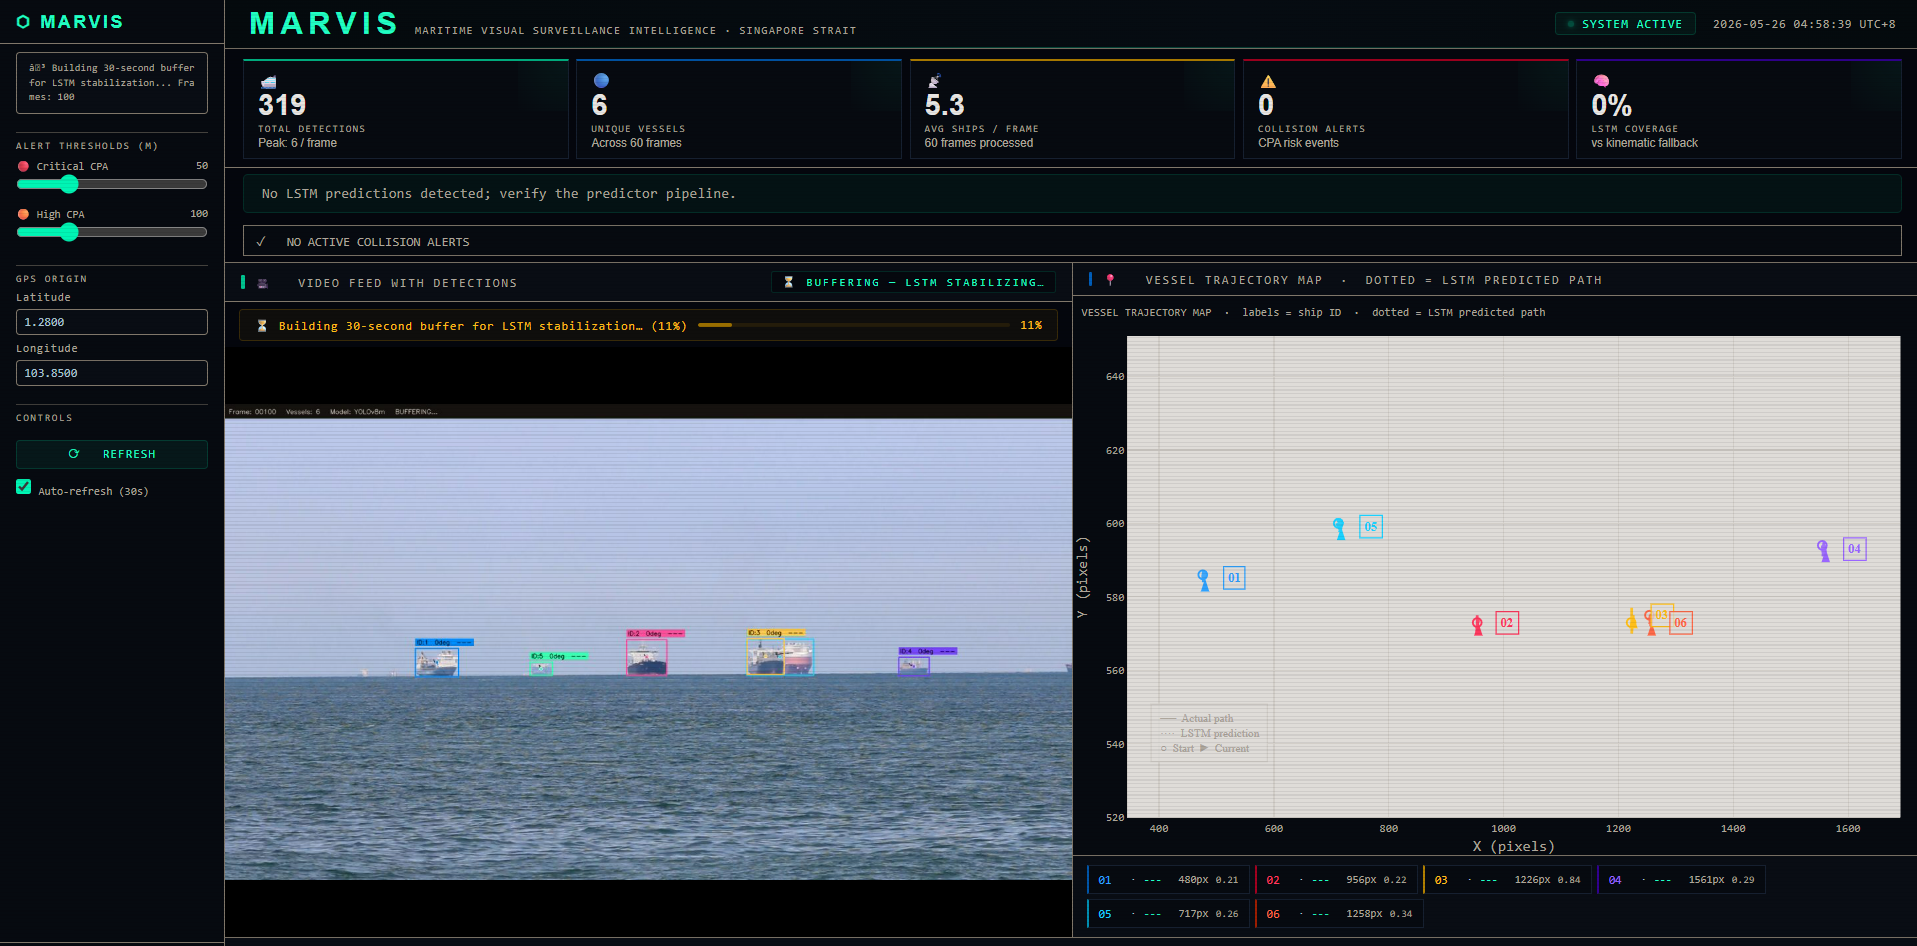
\includegraphics[width=0.95\textwidth]{Chapter5/Figures/dashboard_full.png}
\caption{MARVIS Primary Dashboard Interface showing telemetry, video feed, and real-time mapping.}
\end{figure}

\begin{figure}[H]
\centering
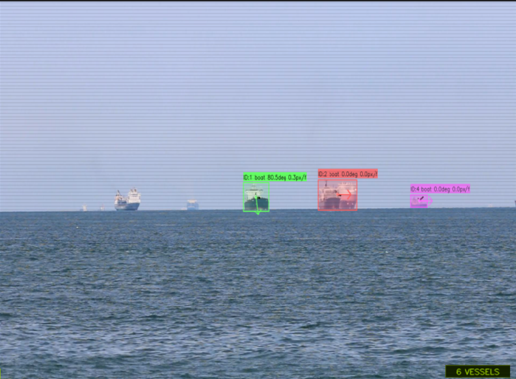
\includegraphics[width=0.95\textwidth]{Chapter5/Figures/detection_output.png}
\caption{Real-time Annotated Video Feed with bounding boxes.}
\end{figure}

\begin{figure}[H]
\centering
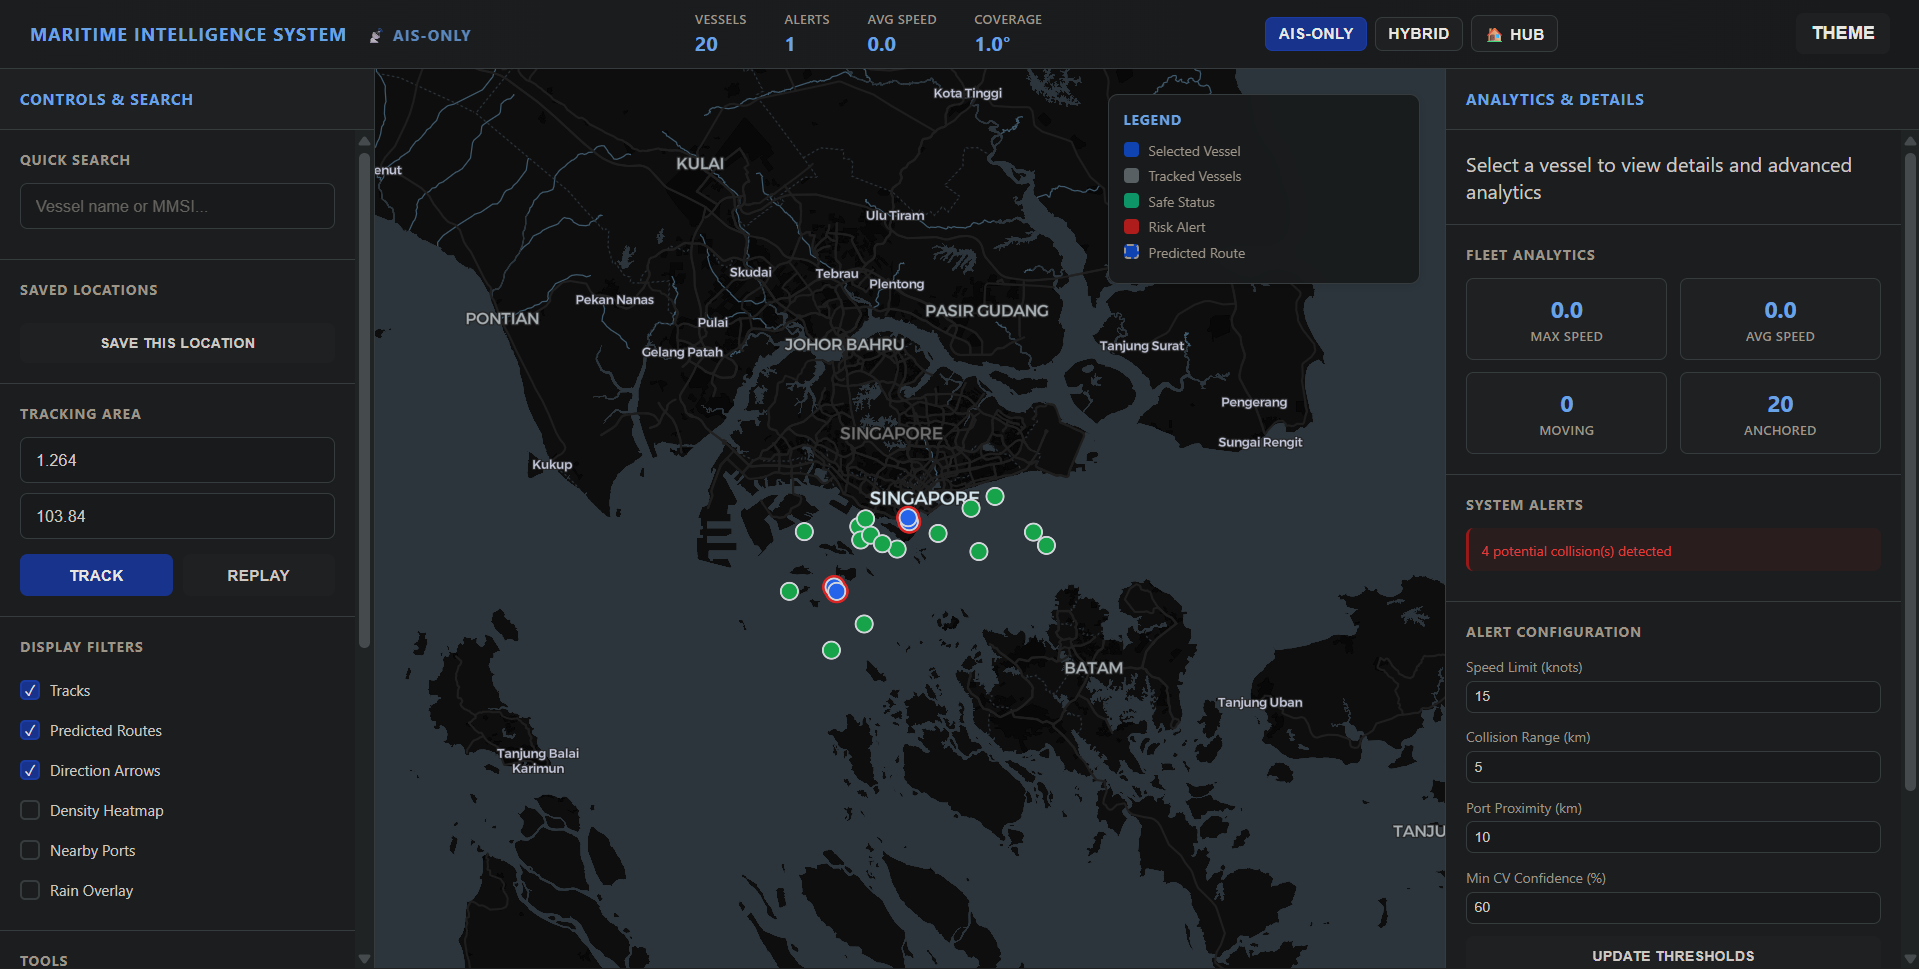
\includegraphics[width=0.95\textwidth]{Chapter5/Figures/ais_fusion_map.png}
\caption{Geospatial AIS Sensor Fusion Map indicating cooperative vessels and potential dark traffic.}
\end{figure}


\section{AIS-Matched Vessel Inference Routing}
The following snippet from \texttt{cv\_matcher.py} illustrates the CV-to-AIS matching logic, which enables the LSTM skip optimization for cooperative vessels.

\begin{tcblisting}{listing only,colback=gray!10!white, breakable, boxsep=0pt,top=1mm,bottom=1mm,left=1mm,right=1mm,
listing options={
language=python,
basicstyle=\small\ttfamily, 
keywordstyle=\color{blue}, 
commentstyle=\color{gray},
backgroundcolor=\color{gray!25},
showspaces=false,
showstringspaces=false,
columns=fullflexible,
escapechar=!}}
def match_cv_to_ais(
    cv_detection: ShipDetection,
    ais_ships: Dict[int, Dict],
    match_radius_km: float = 5.5
) -> Optional[Tuple[int, float]]:
    """Match a camera detection to an AIS ship within a threshold radius."""
    best_match = None
    best_distance = match_radius_km

    for mmsi, ais_ship in ais_ships.items():
        if not ais_ship.get("history") or len(ais_ship["history"]) < 1:
            continue
        
        # Get latest AIS position
        latest_pos = ais_ship["history"][-1]
        distance = calculate_distance_km(
            (cv_detection.gps_lat, cv_detection.gps_lon),
            (latest_pos[1], latest_pos[2])
        )
        
        # Update best match if closer
        if distance < best_distance:
            best_distance = distance
            best_match = (mmsi, distance)
            
    return best_match

def enrich_cv_detection_with_ais(
    cv_detection: ShipDetection, 
    ais_ship: Dict
) -> ShipDetection:
    """Enrich a CV detection with AIS data to skip LSTM prediction."""
    cv_detection.is_matched_to_ais = True
    cv_detection.matched_ais_mmsi = ais_ship.get("mmsi")
    
    # Update with AIS motion data if available
    if "sog" in ais_ship:
        cv_detection.sog = ais_ship["sog"]
    if "cog" in ais_ship: 
        cv_detection.cog = ais_ship["cog"]
        cv_detection.heading = ais_ship["cog"]
        
    return cv_detection
\end{tcblisting}

\section{Dashboard Pipeline Integration Loop}
The following snippet from \texttt{marvis\_api.py} demonstrates the core frame-processing loop where YOLOv8 detection, DeepOCSORT tracking, and LSTM trajectory prediction are integrated into a single real-time pipeline.

\begin{tcblisting}{listing only,colback=gray!10!white, breakable, boxsep=0pt,top=1mm,bottom=1mm,left=1mm,right=1mm,
listing options={
language=python,
basicstyle=\small\ttfamily, 
keywordstyle=\color{blue}, 
commentstyle=\color{gray},
backgroundcolor=\color{gray!25},
showspaces=false,
showstringspaces=false,
columns=fullflexible,
escapechar=!}}
# YOLO detection 
try:
    det_results = yolo_model(
        frame,
        conf    = CONFIDENCE,
        classes = CLASSES,
        verbose = False
    )[0]
    dets = det_results.boxes.data.cpu().numpy()
except Exception as e:
    dets = np.empty((0, 6))

# DeepOcSort tracking
try:
    if len(dets) > 0:
        tracks = tracker.update(dets, frame)
    else:
        tracks = tracker.update(np.empty((0, 6)), frame)
except Exception as e:
    tracks = []

# Build ship list and Predict
for t in (tracks if tracks is not None and len(tracks) > 0 else []):
    try:
        x1, y1, x2, y2 = int(t[0]), int(t[1]), int(t[2]), int(t[3])
        sid            = int(t[4])

        cx = (x1 + x2) // 2
        cy = (y1 + y2) // 2
        history[sid].append((cx, cy))

        smoothed = smooth_history(history[sid])

        # LSTM / kinematic prediction
        if buffer_complete and frame_count % update_frame_interval == 0:
            if lstm_engine:
                lstm_engine.update(str(sid), cx, cy)
                pred, method = lstm_engine.predict(str(sid))
                persistent_predictions[sid] = pred
            else:
                persistent_predictions[sid] = predict_kinematic(smoothed)
        
        predicted_path = persistent_predictions.get(sid, [])
        
    except Exception as e:
        continue
\end{tcblisting}%Appendix for Codes 
		
		\backmatter
		\ifDrf
		\else
		\clearpage
		\addcontentsline{toc}{chapter}{Bibliography}
		\printbibliography%
		\fi
	\end{spacing}
\end{document}
